% !Mode:: "TeX:UTF-8"
%% 请使用 XeLaTeX 编译本文.
% \documentclass{WHUBachelor}% 选项 forprint: 交付打印时添加, 避免彩色链接字迹打印偏淡. 即使用下一行:
\documentclass[forprint]{WHUBachelor}
\usepackage{geometry}
\usepackage{float}
\usepackage{minted}
\usepackage{algorithm}
\usepackage{algorithmicx}
\usepackage{algpseudocode}
\usepackage{amsmath}
\usepackage[lastexercise]{exercise}
\definecolor{bg}{rgb}{0.85,0.85,0.85}
\setminted{fontsize=\small,linenos,frame=single,breaklines}
\linespread{1.8}

\includeonly{lab1, lab2, lab3, lab4, lab5, boot, process, file, struct, eg, io, mem}

\begin{document}
%%%%%%% 下面的内容, 据实填空.

\title{{\Large 哈尔滨工业大学计算机科学与技术学院\\2017年秋季学期《操作系统》} \\ 实验报告}
\author{马玉坤}                            % 作者名字
\Cmajor{计算机科学与技术}                  % 专业中文名
\Cschoolname{计算机科学与技术系}          % 学院名
\date{二〇一八年一月}                    % 日期, 要注意和英文日期一致!!
\teammates{李伟枫,许浩禹,张宁}
\StudentNumber{1150310618}
\Phone{18845895386}
\Csupervisor{曲明成}
\newcommand{\shell}[1]{\indent\indent\texttt{\footnotesize\# #1}\\}

%-----------------------------------------------------------------------------
\pdfbookmark[0]{封面}{title}         % 封面页加到 pdf 书签
\maketitle
\frontmatter
\pagenumbering{Roman}              % 正文之前的页码用大写罗马字母编号.
%-----------------------------------------------------------------------------
% !Mode:: "TeX:UTF-8"

%%% 此部分需要自行填写: (1) 中文摘要及关键词 (2) 英文摘要及关键词

%%======中文摘要===========================%
\begin{cnabstract}
  在本次CPU设计过程中,本人在两位实验课老师和Digilent社区的帮助下,设计了一个可在Nexys 4 DDR上运行的,有固定指令周期的且支持十条指令的精简指令集 (RISC) 处理器。本文详细介绍了本人在计算机设计与实践实验课上完成计算机设计与实践实验5的相关设计。本文内容包括: (1) CPU的顶层设计; (2) CPU各个模块,包括取指模块、运算模块、访存模块、回写模块、内存控制以及IO控制若干个模块的内部设计; (3)进行CPU设计及实现过程中遇到的问题与解决方法; (4) Digilent Nexys 4 DDR FPGA的简单介绍。

\end{cnabstract}
\par
\vspace*{2em}


%%%%--  关键词 -----------------------------------------%%%%%%%%
%%%%-- 注意: 每个关键词之间用“;”分开,最后一个关键词不打标点符号
\cnkeywords{中央处理器; CPU; FPGA; VHDL; 计算机设计与实践 }
    % 加入摘要, 申明.
%==========================把目录加入到书签==============================%%%%%%
\pdfbookmark[0]{目录}{toc}
\tableofcontents
\mainmatter %% 以下是正文
%%%%%%%%%%%%%%%%%%%%%%%%%%%--------main matter-------%%%%%%%%%%%%%%%%%%%%%%%%%%%%%%%%%%%%

\chapter{xv6实验系统简述}

xv6\cite{xv6-doc}\cite{xv6-github}是由麻省理工学院(MIT)为操作系统工程的课程(代号6.828),开发的一个教学目的的操作系统。xv6是在x86处理器上(x即指x86)用ANSI标准C重新实现的Unix第六版(Unix V6,通常直接被称为V6)。

截至2017年12月,xv6的最新版本为rev10。

xv6使用GNU C编译器编译,并支持ELF可执行文件格式。(由于OS X不支持ELF可执行文件,所以需要交叉编译器\footnote{cross-compiler})。

xv6总代码行数只有9299行\footnote{\url{https://pdos.csail.mit.edu/6.828/2017/xv6/xv6-rev10.pdf}}。但是麻雀虽小,五脏俱全,包括了Unix的重要概念和组织结构,因此我个人认为特别适用于本科的操作系统教学中。

\begin{figure}[H]
  \centering
  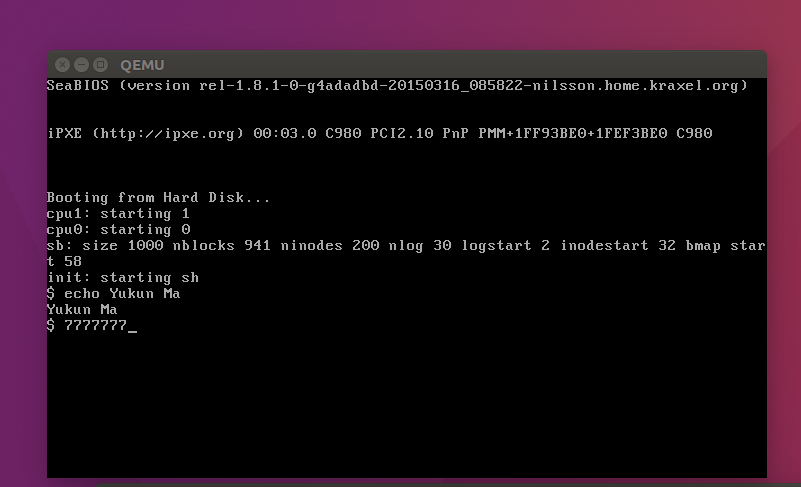
\includegraphics[width=6in]{figures/xv6/show.png}
  \caption{xv6运行截图}\label{fig:xv6:show}
\end{figure}

\chapter{xv6环境配置}

\section{系统环境}

建议使用32位Linux操作系统,64位Linux操作系统也可以。

这里我在Windows上用Virtual Box安装了Ubuntu 14.04 32位版。

\begin{figure}[H]
  \centering
  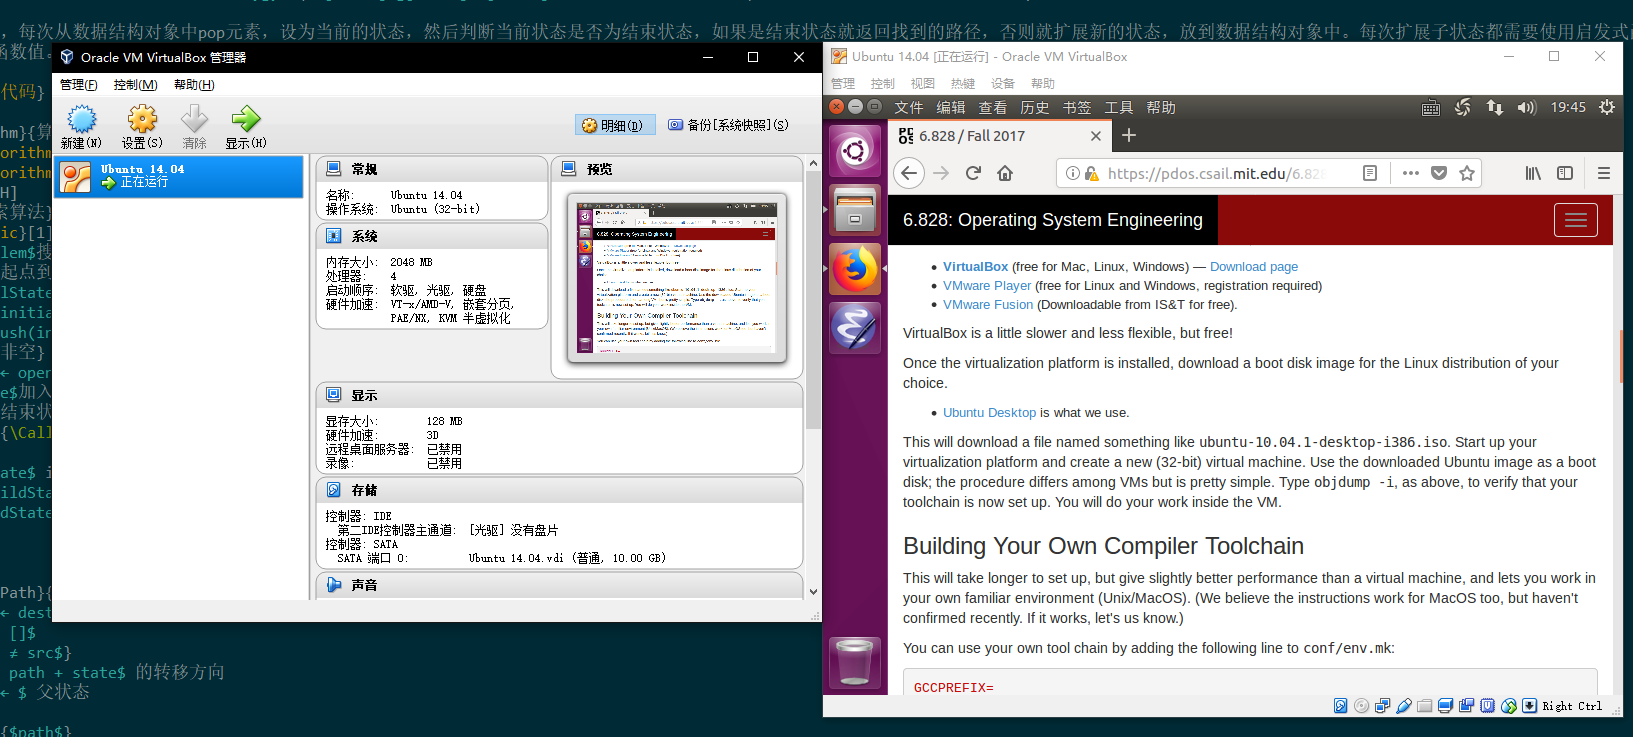
\includegraphics[width=6in]{figures/prep/vm.png}
  \caption{Ubuntu虚拟机}\label{fig:prep:vm}
\end{figure}

\section{编译环境}

先用以下命令检查编译环境是否装好。

\shell{objdump -i}

第二行应该是\textbf{elf32-i386}。

\shell{gcc -m32 -print-libgcc-file-name}

这个命令应该打印一些类似于\textbf{The command should print something like /usr/lib/gcc/i486-linux-gnu/version/libgcc.a or /usr/lib/gcc/x86\_64-linux-gnu/version/32/libgcc.a}的东西。

还需要安装GCC(GNU C Compiler)。

\shell{sudo apt-get install -y build-essential gdb}

如果是64位系统,还需要:

\shell{sudo apt-get install gcc-multilib}

\begin{figure}[H]
  \centering
  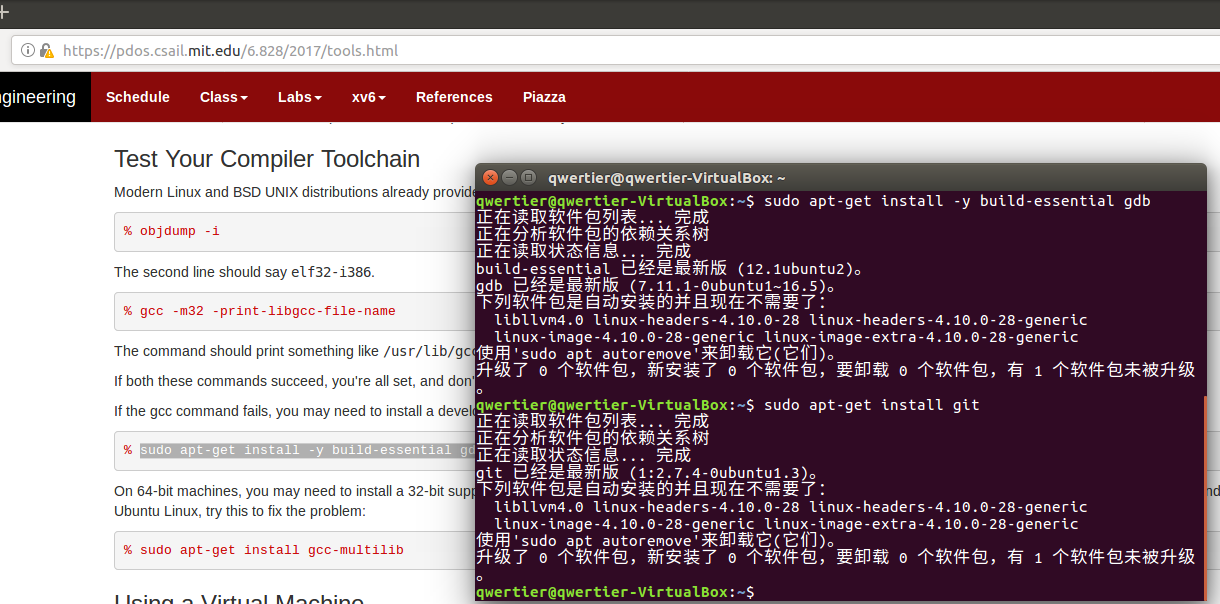
\includegraphics[width=6in]{figures/prep/tools.png}
  \caption{安装所需的软件}\label{fig:prep:tools}
\end{figure}

\section{安装QEMU}

实验需要用到QEMU模拟器,但是普通的QEMU会出bug,所以需要修改版的。

如图\ref{fig:prep:qemu},先要使用git clone下修改版QEMU。

\shell{git clone https://github.com/geofft/qemu.git}

\begin{figure}[H]
  \centering
  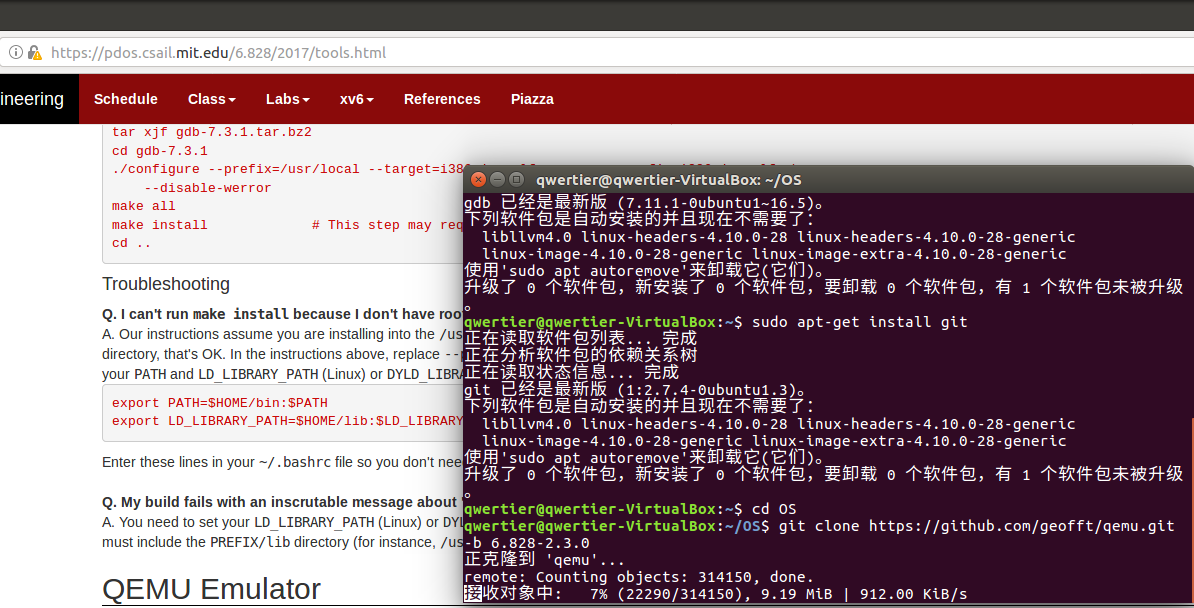
\includegraphics[width=6in]{figures/prep/qemu.png}
  \caption{git clone QEMU的过程}\label{fig:prep:qemu}
\end{figure}

如图\ref{fig:prep:qemu_config},运行进入到qemu路径下,使用configure。

\shell{./configure --disable-kvm --target-list="i386-softmmu x86\_64-softmmu"}

\begin{figure}[H]
  \centering
  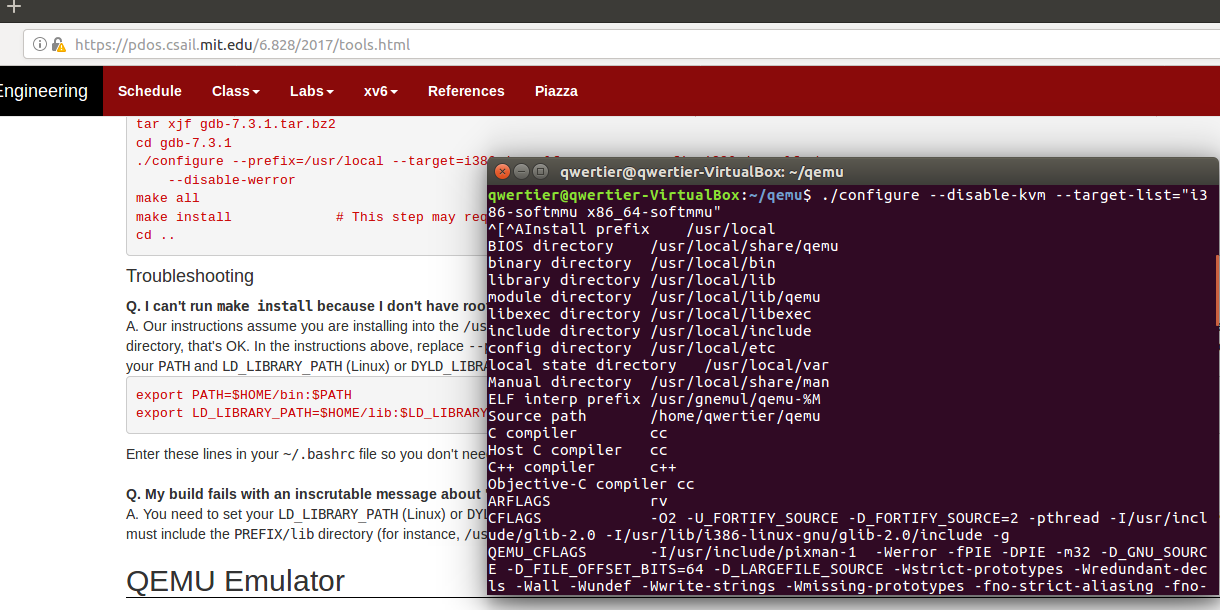
\includegraphics[width=6in]{figures/prep/qemu_config.png}
  \caption{configure QEMU的过程}\label{fig:prep:qemu_config}
\end{figure}

如图\ref{fig:prep:qemu_make},使用make命令编译qemu。

\shell{sudo make \&\& sudo make install}

\begin{figure}[H]
  \centering
  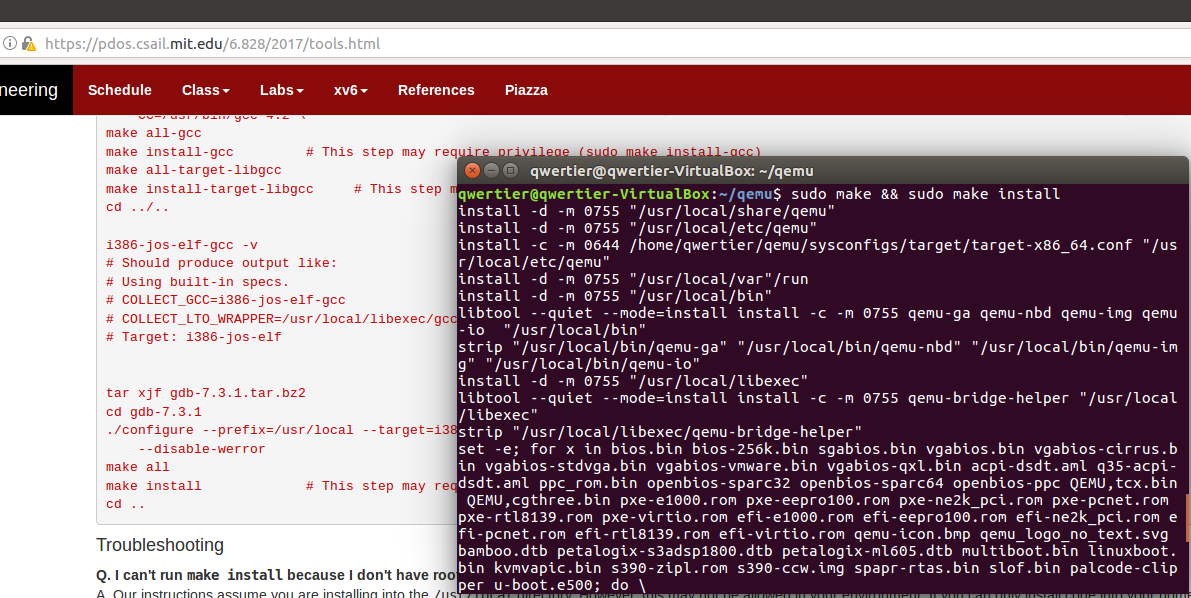
\includegraphics[width=6in]{figures/prep/qemu_make.png}
  \caption{make QEMU的过程}\label{fig:prep:qemu_make}
\end{figure}

然后QEMU就安装成功了。

\chapter{实验过程}

\begin{ExerciseList}
\section{Lab 1: Booting a PC}

\subsection{实验简介}

本实验被分为三个部分。第一个部分主要集中在熟悉x86汇编语言、QEMU模拟器以及PC的启动步骤。第二个部分通过实践来对系统内核的boot loader进一步了解。第三部分来深入研究JOS的系统内核。

\subsection{实验目的}

\begin{enumerate}
\item 熟悉(复习)x86汇编语言,为接下来的工作打好基础
\item 了解开发环境的使用方法,尤其是QEMU模拟器的使用
\item 对PC启动的过程有更清晰的了解
\item 了解堆栈,清楚函数调用时的栈帧结构
\end{enumerate}

\subsection{实验内容}

\subsubsection{准备}

装完QEMU模拟器之后,如果想做后续的实验,还需要下载JOS的残缺的源码(需要我们在后面填充内容)。

\shell{git clone https://pdos.csail.mit.edu/6.828/2017/jos.git lab}
\shell{cd lab}

进入lab目录之后,如图\ref{fig:lab1:jos},我们可以看到lab目录的大致结构。

\begin{figure}[H]
  \centering
  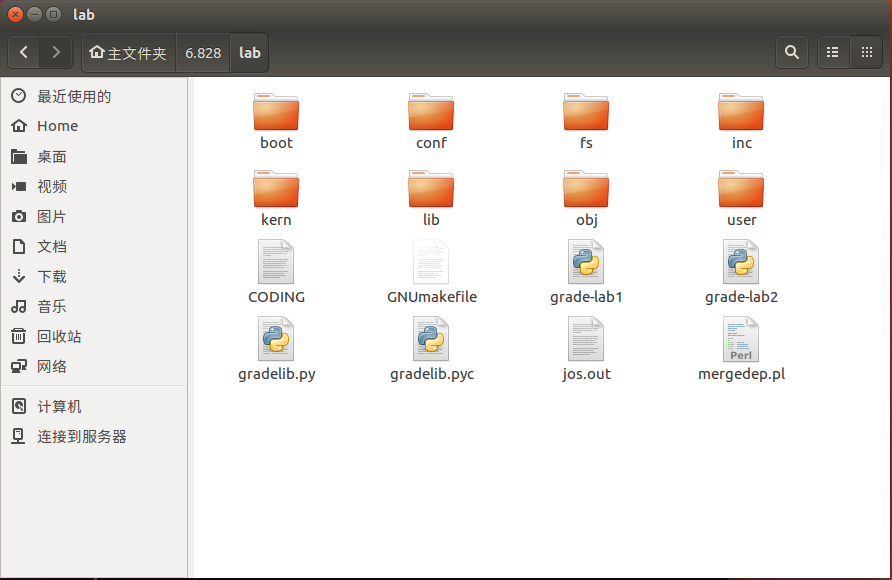
\includegraphics[width=6in]{figures/lab1/jos.png}
  \caption{lab目录的结构}\label{fig:lab1:jos}
\end{figure}

在lab目录下运行如下命令:

\shell{make qemu}

如图\ref{fig:lab1:make_qemu},就能用QEMU运行JOS。

\begin{figure}[H]
  \centering
  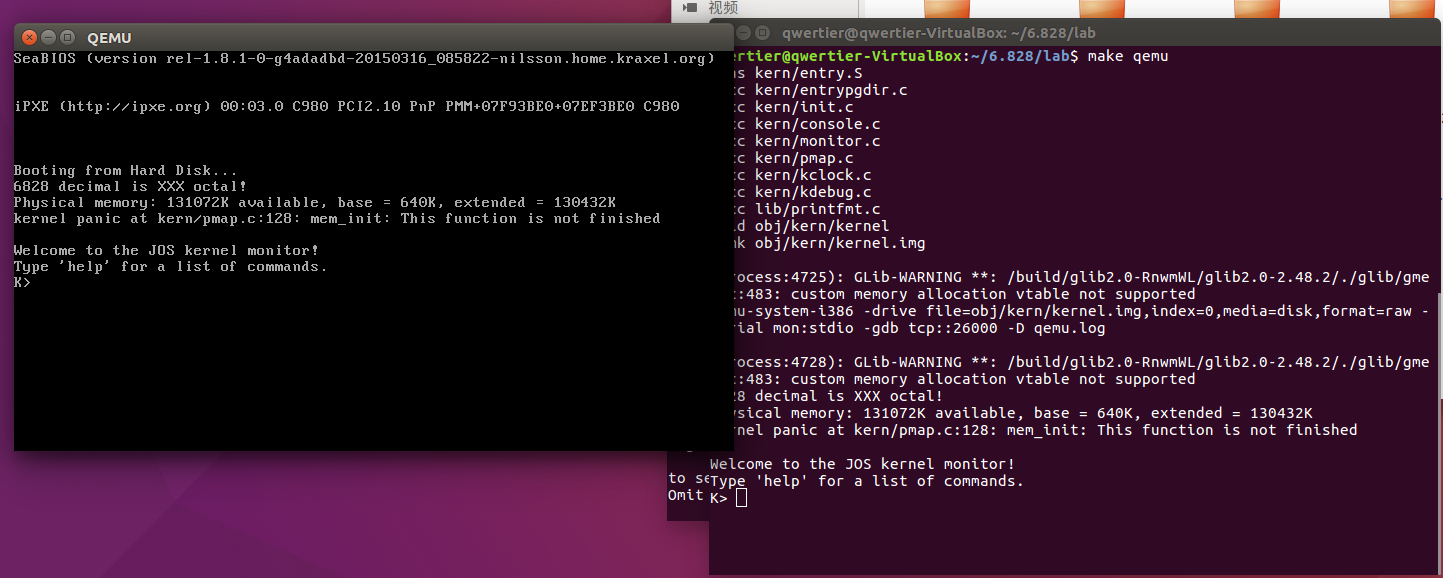
\includegraphics[width=6in]{figures/lab1/make_qemu.png}
  \caption{lab目录的结构}\label{fig:lab1:make_qemu}
\end{figure}

\subsubsection{第一部分:启动PC}

\Exercise{熟悉汇编语言}

汇编语言的英文资料可以在\url{https://pdos.csail.mit.edu/6.828/2017/reference.html}找到。

\Exercise{使用GDB的单步调试(si)语句追踪ROM BIOS,然后猜测它在做什么。}

在一个终端中输入 make qemu-gdb , 另一个终端输入 make gdb 。开始调试程序。

\shell{[f000:fff0] 0xffff0: ljmp \$0xf000,\$0xe05b}

是GDB反汇编出的第一条执行指令,这条指令表明了:IBM PC 执行的起始物理地址为 0x000ffff0,PC 的偏移方式为 CS = 0xf000,IP = 0xfff0。

\begin{figure}[H]
  \centering
  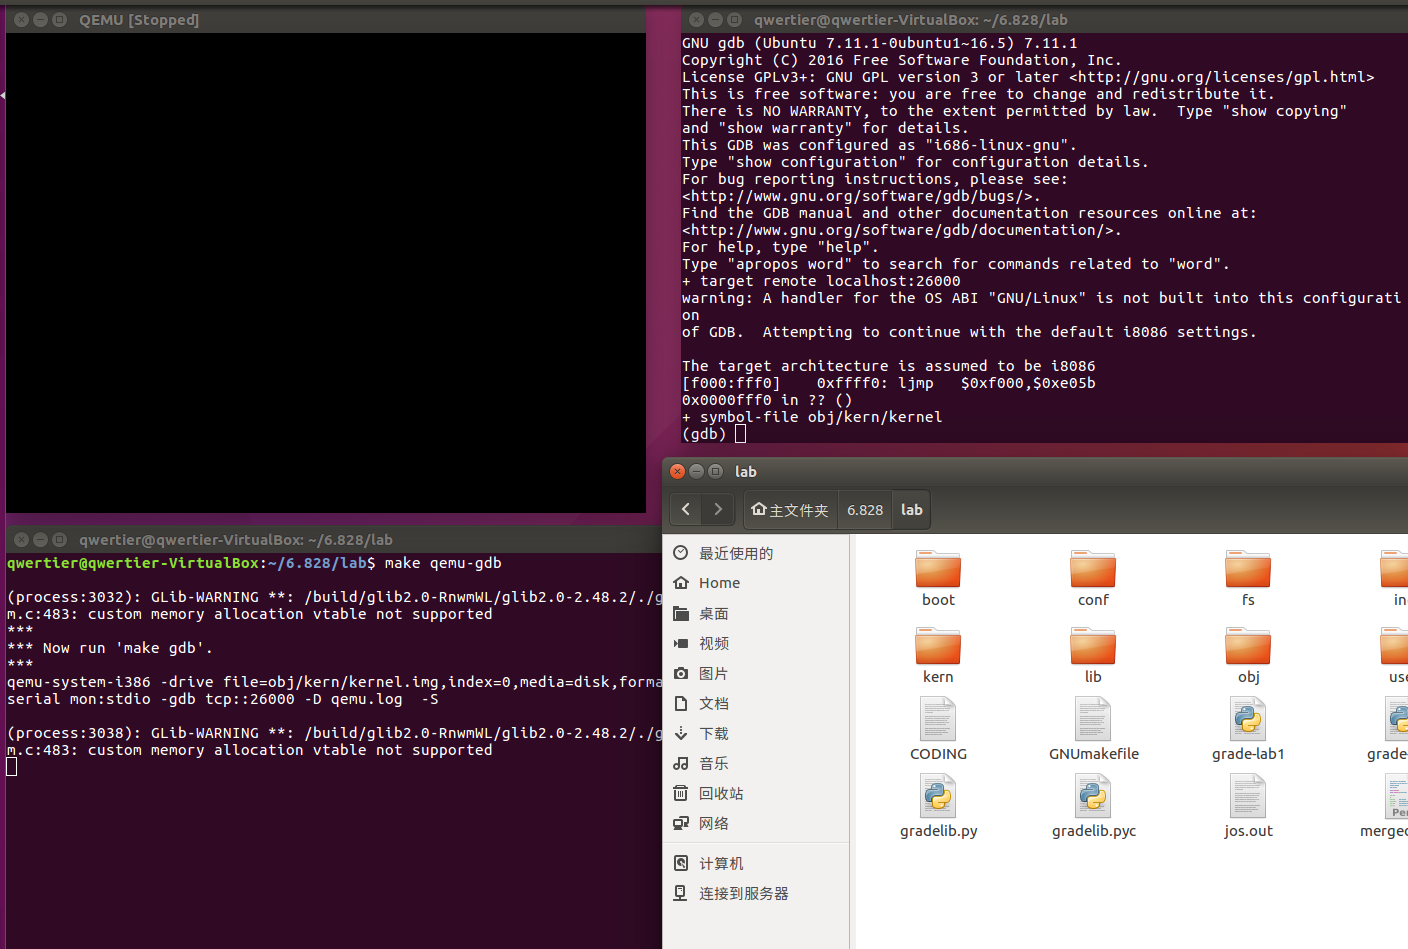
\includegraphics[width=6in]{figures/lab1/gdb.png}
  \caption{使用gdb调试第一条指令}\label{fig:lab1:gdb}
\end{figure}

第一条指令执行的是 jmp指令,跳转到段地址 CS = 0xf000,IP = 0xe05b。QEMU模拟了8088处理器的启动,当启动电源,BIOS最先控制机器,这时还没有其他程序执行,之后处理器进入实模式也就是设置 CS 为 0xf000,IP 为 0xfff0。在启动电源也就是实模式时,地址转译根据这个公式工作:物理地址 = 16 * 段地址 + 偏移量。所以 PC 中 CS 为 0xf000 IP 为 0xfff0 的物理地址为:

\begin{align}
   & 16 * 0xf000 + 0xfff0\\
   = & 0xf0000 + 0xfff0\\
   = & 0xffff0
\end{align}

0xffff0 在 BIOS (0x100000) 的结束地址之前。

当BIOS开始运行时,它会建立中断描述表\footnote{Interrupt Descriptor Table}然后初始化众多设备(例如显示器)。这就是当你从QEMU中看到''Starting SeaBIOS''的时候。

当所有的其他设备都初始化完成了,BIOS会继续找可以启动的设备(例如硬盘、CD-ROM)。最后它会找到可启动盘,接着BIOS从启动盘中读出boot loader然后转移控制权。

\subsubsection{第二部分:The Boot Loader}

\Exercise{在\url{https://pdos.csail.mit.edu/6.828/2017/labguide.html}熟悉一下 GDB 的指令。然后在0x7c00处设一个断点,执行到断点。进入boot/boot.S,参考源代码和反汇编代码 \emph{obj/boot/boot.asm}来跟踪。追踪到bootmain函数中,而且还要具体追踪到readsect()子函数里面。找出和readsect()c语言程序的每一条语句所对应的汇编指令,回到bootmain(),然后找出把内核文件从磁盘读取到内存的那个for循环所对应的汇编语句。找出当循环结束后会执行哪条语句,在那里设置断点,继续运行到断点,然后运行完所有的剩下的语句。}

\textbf{\$[0:7c2d] => 0x7c2d: ljmp \$0x8,\$0x7c32}这条指令之后,也就是 boot.S 中的\textbf{ ljmp \$PROT\_MODE\_CSEG, \$protcseg} ,地址符号就变成 0x7c32 了。

首先查看boot.S文件,在开头可以看到如下代码,cld 是串操作指令,用来操作方向标志位DF,使DF=0。

\begin{minted}{ASM}
start:
  .code16
  cli
  cld                         # String operations increment
\end{minted}

如以下代码,\textbf{inb \$0x64,\%al}把$0x64$端口(8042键盘控制器)的状态写入al中(inb代表IO端口读), 之后 \textbf{testb \$0x2,\%al}判断al的第二位是否为0,不为0就循环执行seta20.1。这里第二位代表输入缓冲区是否满了。接着$0xd1$放入$0x64$端口。最后将$0xdf$放入0x60端口,代表开启A20地址线了。

\begin{minted}{ASM}
  # Enable A20:
  #   For backwards compatibility with the earliest PCs, physical
  #   address line 20 is tied low, so that addresses higher than
  #   1MB wrap around to zero by default.  This code undoes this.
seta20.1:
  inb     $0x64,%al               # Wait for not busy
  testb   $0x2,%al
  jnz     seta20.1

  movb    $0xd1,%al               # 0xd1 -> port 0x64
  outb    %al,$0x64

seta20.2:
  inb     $0x64,%al               # Wait for not busy
  testb   $0x2,%al
  jnz     seta20.2

  movb    $0xdf,%al               # 0xdf -> port 0x60
  outb    %al,$0x60
\end{minted}

通过如下代码,开始调用\emph{bootmain}函数。

\begin{minted}{ASM}
  # Set up the stack pointer and call into C.
  movl    $start, %esp
  call bootmain
\end{minted}

如下代码所示,在bootmain函数中,调用readseg函数。该函数有三个参数,分别是物理地址、页大小和偏移量。

\begin{minted}{ASM}
  # read 1st page off disk
  readseg((uint32_t) ELFHDR, SECTSIZE*8, 0);
    push   $0x0
    push   $0x1000
    push   $0x10000
    call   7cdc <readseg>
\end{minted}

如下指令用于加载程序段。

\begin{minted}{ASM}
    mov    0x1001c,%eax
    movzwl 0x1002c,%esi
    lea    0x10000(%eax),%ebx
    shl    $0x5,%esi
    add    %ebx,%esi
\end{minted}

\Exercise{了解C语言中关于指针的知识(已经学过了)}

为了理解 boot/main.c, 需要了解ELF二进制文件。编译并链接比如JOS内核这样的C程序,编译器会将源文件(.c)转为包含汇编指令的目标文件(.o)。接着链接器把所有的目标文件组合成一个单独的二进制镜像(binary image),比如 obj/kern/kernel,这种文件就是ELF(是可执行可链接形式的缩写)。

当前只需要知道,可执行的ELF文件由带有加载信息的头,多个程序段表组成。每个程序段表是一个连续代码块或者数据,它们要被加载到内存具体地址中。boot loader 不修改源码和数据,直接加载到内存中并运行。

ELF开头是固定长度的 ELF头,之后是一个可变长度的程序头,它列出了需要加载的程序段。ELF头的定义在 inc/elf.h 中。主要学习以下3个程序段:

\begin{itemize}
\item .text: 程序执行指令
\item .rodata:只读数据,比如ASCII字符串
\item .data: 存放程序初始化的数据段,比如有初始值的全局变量。
\end{itemize}

使用以下命令可以查看\emph{obj/kern/kernel}文件的ELF头的相关信息,结果如图\ref{fig:lab1:kernel_elf}。

\shell{objdump -h obj/kern/kernel}

\begin{figure}[H]
  \centering
  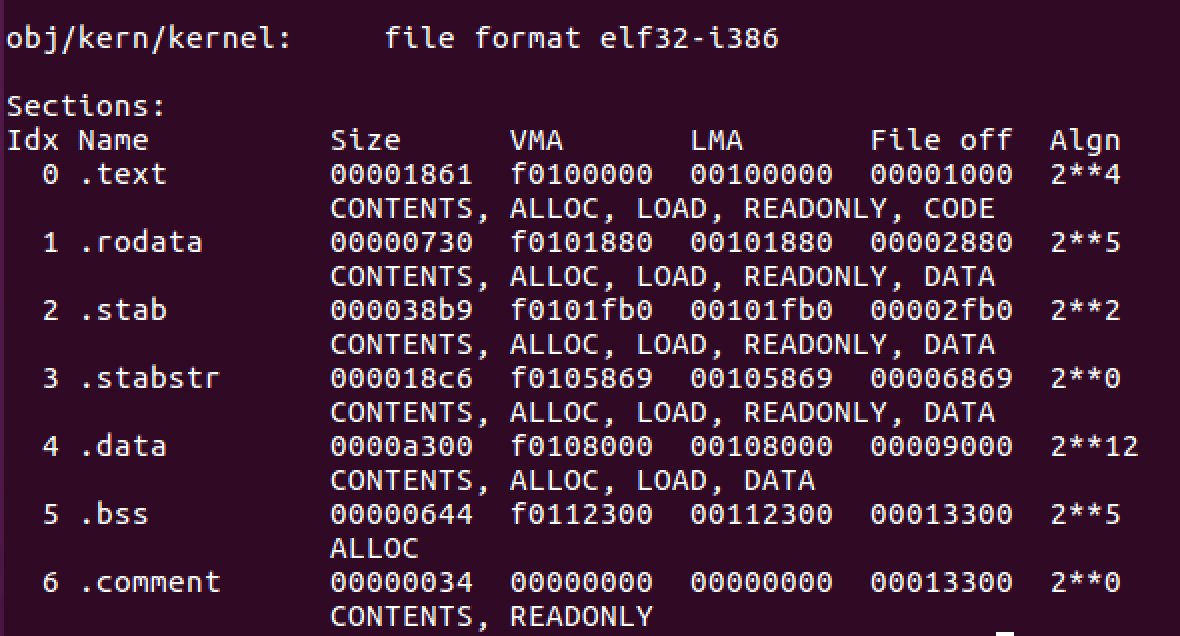
\includegraphics[width=6in]{figures/lab1/kernel_elf.png}
  \caption{\emph{obj/kern/kernel}文件的ELF头}\label{fig:lab1:kernel_elf}
\end{figure}

使用以下命令可以查看\emph{obj/boot/boot.out}文件的ELF头的相关信息,结果如图\ref{fig:lab1:boot_elf}所示。

\shell{objdump -h obj/boot/boot.out}

\begin{figure}[H]
  \centering
  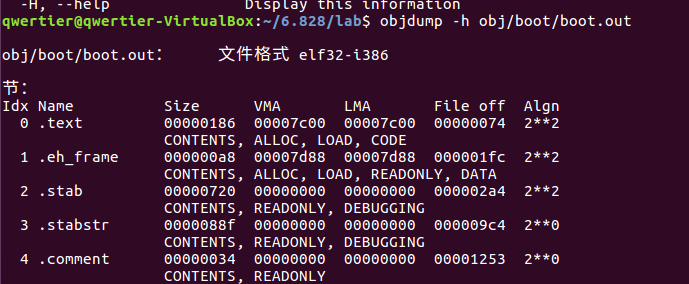
\includegraphics[width=6in]{figures/lab1/boot_elf.png}
  \caption{\emph{obj/boot/boot.out}文件的ELF头}\label{fig:lab1:boot_elf}
\end{figure}

\Exercise{修改\emph{boot/Makefrag},使得boot loader的加载地址出错,找到第一条出错的指令。\footnote{做完之后需要使用\textbf{make clean}命令之后再make。}}

查看\emph{boot/Makefrag}文件,文件内容如下所示。可以发现\textbf{-Ttext}后面的参数就是入口地址。如果把这个值修改为$0x8C00$,保存后回到lab1文件夹下进行make。

\begin{minted}{Makefile}
$(OBJDIR)/boot/boot: $(BOOT_OBJS)
    @echo + ld boot/boot
    $(V)$(LD) $(LDFLAGS) -N -e start -Ttext 0x7C00 -o $@.out $^
    $(V)$(OBJDUMP) -S $@.out >$@.asm
    $(V)$(OBJCOPY) -S -O binary -j .text $@.out $@
    $(V)perl boot/sign.pl $(OBJDIR)/boot/boot

\end{minted}

如下代码,查看\emph{obj/boot/boot.asm}会发现起始地址从原来的00007c00 变为 00008c00。虽然此时在0x7c00处打断点然后运行时正常的,但是继续si以后会在 \textbf{[0:7c2d] => 0x7c2d: ljmp \$0x8,\$0x8c32} 出循环,同时qemu端口出现了错误。因为不能ljmp到\$0x7c32而是调到了\$0x8c32,所以无法执行正确的指令。查看 boot.asm 可以知道上面这个指令是 \textbf{ljmp \$PROT\_MODE\_CSEG, \$protcseg},是为了进入32位模式的。

\begin{minted}{ASM}
.set CR0_PE_ON,      0x1         # protected mode enable flag

.globl start
start:
  .code16                     # Assemble for 16-bit mode
  cli                         # Disable interrupts
    8c00:    fa                       cli
  cld                         # String operations increment
    8c01:    fc                       cld
\end{minted}

\Exercise{使用GDB的\textbf{x}\footnote{参考\url{https://sourceware.org/gdb/current/onlinedocs/gdb/Memory.html}}命令可以可以查看内存信息。重启QEMU,当BIOS进入boot loader时检查0x00100000处的8个字节,然后在boot loader进入内核时再看一次。为什么两者有不同?在第二个端点处到底有什么?}

在0x7c00处设置断点,然后运行到断点处,使用 x/8x 0x100000 可以看到如图\ref{fig:lab1:gdb_x}

\begin{figure}[H]
  \centering
  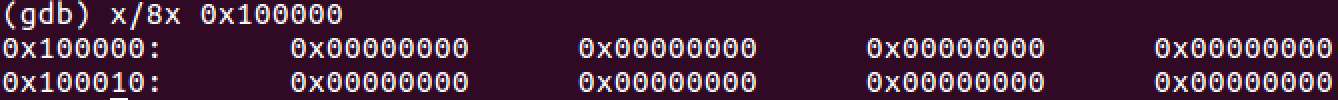
\includegraphics[width=6in]{figures/lab1/gdb_x.png}
  \caption{内存截图}\label{fig:lab1:gdb_x}
\end{figure}

根据之前的看到程序入口点是 0x10000c ,所以在 0x10000c 处打断点运行,如图\ref{fig:lab1:gdb_x2}同样可以看到

\begin{figure}[H]
  \centering
  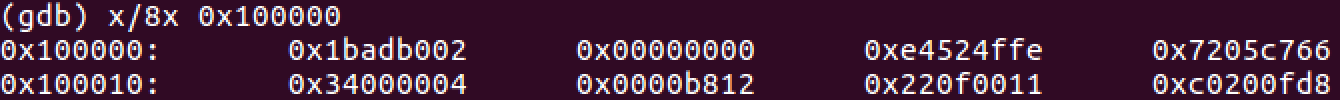
\includegraphics[width=6in]{figures/lab1/gdb_x2.png}
  \caption{内存截图}\label{fig:lab1:gdb_x2}
\end{figure}

$0x100000$处存放的其实就是程序指令段,也就是说 bootmain 函数会把内核的程序段送到内存$0x100000$处。



\subsubsection{第三部分:内核}

boot loader 的链接地址和加载地址是一样的,然而 kernel 的链接地址和加载地址有些差异。查看 kern/kernel.ld 可以发现内核地址在 0xF0100000。

操作系统内核通常被链接并且运行在非常高的虚拟地址,比如文件里看到的 0xf0100000,为了让处理器虚拟地址空间的低地址部分给用户程序使用。

许多机器没有地址为 0xf0100000 的物理内存,所以内核不能放在那儿。因此使用处理器内存管理硬件将虚拟地址 0xf0100000 (内核希望运行的链接地址)映射到物理地址 0x00100000 (boot loader加载内核后所放的物理地址)。尽管内核虚拟地址很高,但加载进物理地址位于1MB的地方仅仅高于BIOS的ROM。这需要PC至少有1MB的物理内存。

在下一个lab,会映射物理地址空间底部256MB,也就是 0x00000000 到 0x0fffffff,到虚拟地址 0xf0000000 ~ 0xffffffff。所以JOS只使用物理内存开始的256MB。

目前,只是映射了物理内存开始的4MB, 使用手写的静态初始化页目录和也表在 kern/entrypgdir.c。当 kern/entry.S 设置 CR0\_PG 标记,存储器引用就变为虚拟地址,即存储器引用是由虚拟存储器硬件转换为物理地址的虚拟地址。entry\_pgdir 将虚拟地址 0xf0000000 ~ 0xf0400000 转换为物理地址 0x00000000 ~ 0x00400000,虚拟地址 0x00000000 ~ 0x00400000 也转换为物理地址 0x00000000 ~ 0x00400000。任何不在这两个范围内的虚拟地址会导致硬件异常。

\Exercise{追踪JOS内核并停在 movl \%eax, \%cr0。查看内存 0x00100000 和 0xf0100000。接着使用 stepi 来看上面两个地址里内容的变化。若注释了 kern/entry.S 的 movl \%eax, \%cr0, 查看第一个出现问题的指令是什么。}

查看 kern/entry.S 发现 \_start 是ELF入口点,exercise 5 提到了入口点是 0x0010000c. 所以在0x0010000c处打断点。

\shell{(gdb) b *0x0010000c}

注释 \textbf{movl \%eax, \%cr0} 后,make clean 之后重新编译,再运行。一步步 si 后出现了问题。

\begin{figure}[H]
  \centering
  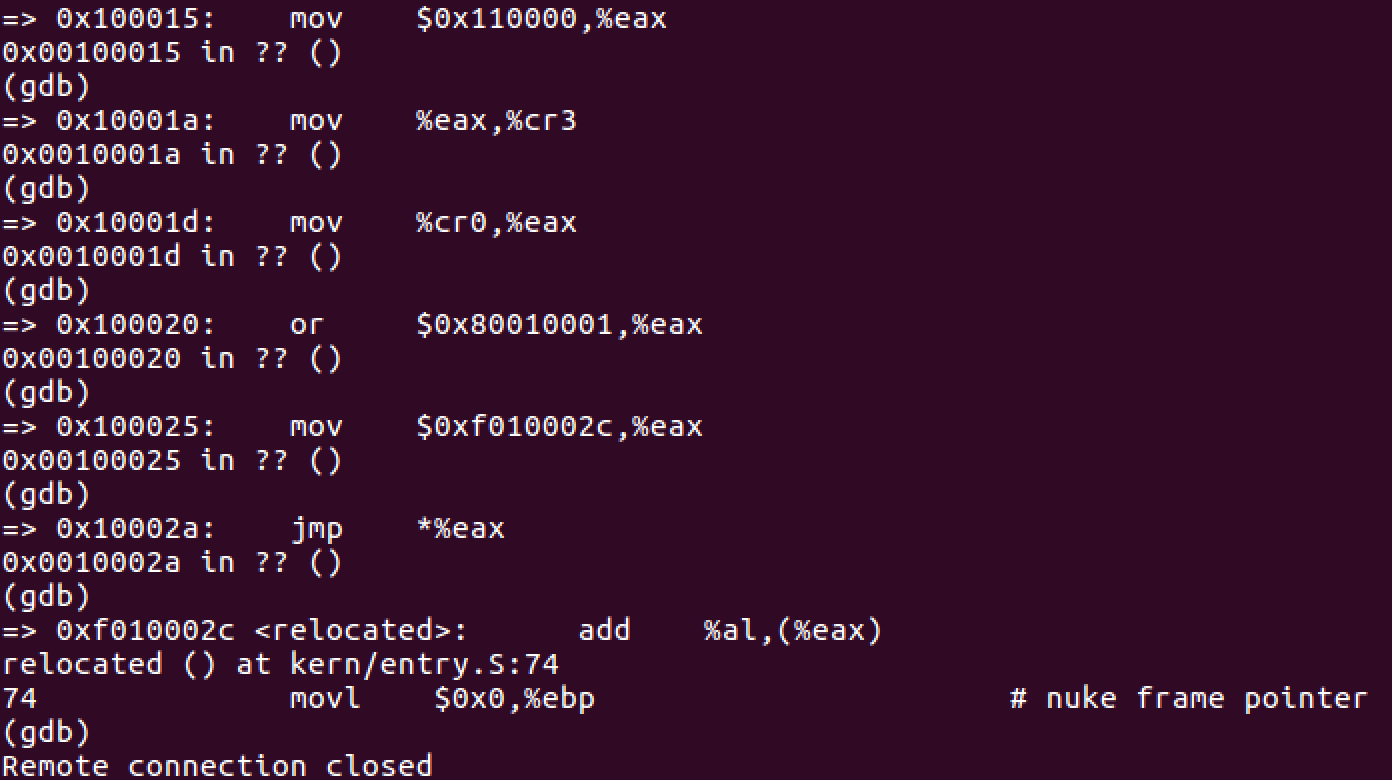
\includegraphics[width=6in]{figures/lab1/ex7.png}
  \caption{GDB截图}\label{fig:lab1:ex7}
\end{figure}

在0x10002a处的jmp指令,要跳到 0xf010002c 处, 然而因为没有分页管理,不会进行虚拟地址映射到物理地址的转化,如图\ref{fig:lab1:fatal},在另一个窗口可以看到错误信息,访问地址超出内存。

\begin{figure}[H]
  \centering
  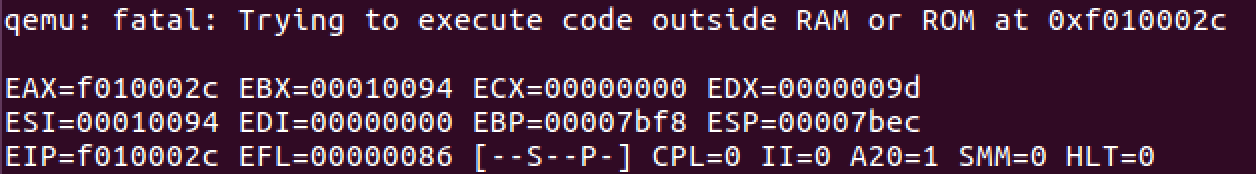
\includegraphics[width=6in]{figures/lab1/fatal.png}
  \caption{错误截图}\label{fig:lab1:fatal}
\end{figure}

\Exercise{完成指定输出''\%o''格式字符串的代码。}

要去实现\%o的格式化输出。在 lib/printfmt.c 可以看到要填写的地方。参考上面 case 'u' 的写法。

\begin{minted}{C}
case 'o':
    num = getuint(&ap, lflag);
    base = 8;
    goto number;
\end{minted}

修改完以后保存,make clean 之后运行,会发现启动以后,如图\ref{fig:lab1:printf},qemu里JOS启动时会出现这样一行字。

\begin{figure}[H]
  \centering
  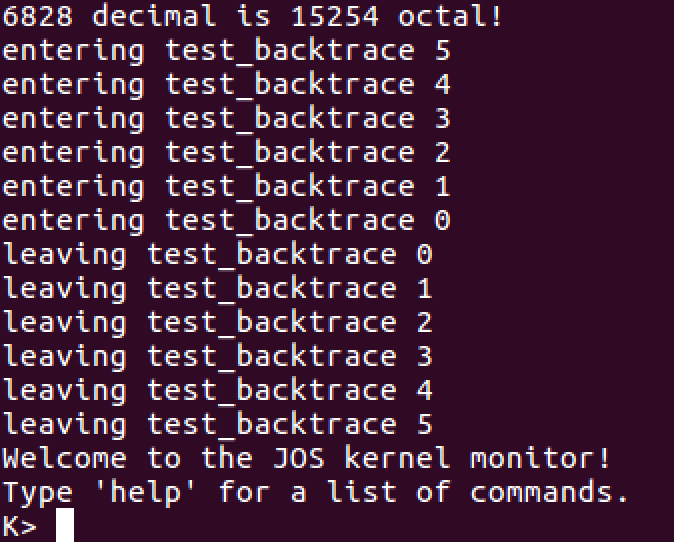
\includegraphics[width=6in]{figures/lab1/printf.png}
  \caption{错误截图}\label{fig:lab1:printf}
\end{figure}

\Exercise{研究内核是在哪初始化堆栈,找出堆栈存放在内存的位置。内核是如何保存一块空间给堆栈的?堆栈指针指向这块区域的哪儿?}

看了几个文件以后,发现在 kern/entry.S 中提到了设置堆指针和栈指针。

\begin{minted}{ASM}
    # Clear the frame pointer register (EBP)
    # so that once we get into debugging C code,
    # stack backtraces will be terminated properly.
    movl    $0x0,%ebp            # nuke frame pointer

    # Set the stack pointer
    movl    $(bootstacktop),%esp
\end{minted}

为了查看堆的位置,所以要使用gdb,同样还是 b *0x10000c 打断点进入 entry。 si 一步步执行,在 0x10002d: jmp *\%eax 之后,下一条指令变为 0xf010002f <relocated>: mov \$0x0,\%ebp。其实地址应该还是 0x10002f,所以这里的 0xf010002f 是因为开启的虚拟地址。

通过 gdb 发现 0xf0100034 <relocated+5>: mov \$0xf0110000,\%esp, 也就是说\%esp也就是bootstacktop的值为0xf0110000。其中 kern/entry.S 的 KSTKSIZE 应该就是堆栈的大小,通过跳转,发现在 inc/memlayout.h 里提到了堆栈。

\begin{minted}{C}
// Kernel stack.
#define KSTACKTOP    KERNBASE
#define KSTKSIZE    (8*PGSIZE)           // size of a kernel stack
#define KSTKGAP        (8*PGSIZE)           // size of a kernel stack guard
\end{minted}

\Exercise{研究 obj/kern/kernel.asm 中 test\_backtrace 向堆栈里压入的信息。}

使用单步调试和 info registers 来查看esp和ebp的变化。

运行test\_backtrace前寄存器如下所示,

{\noindent\small esp            0xf010ffdc    0xf010ffdc\\
ebp            0xf010fff8    0xf010fff8
}

现在需要实现mon\_backtrace()这个函数,需要显示ebp,eip 和 args。ebp是基址指针,eip是返回指令指针。简单实现backtrace,实现效果如下:

{\noindent\small Stack backtrace:
  ebp f0109e58  eip f0100a62  args 00000001 f0109e80 f0109e98 f0100ed2 00000031\\
  ebp f0109ed8  eip f01000d6  args 00000000 00000000 f0100058 f0109f28 00000061
  ...}

代码:

\begin{minted}{C}
int
mon_backtrace(int argc, char **argv, struct Trapframe *tf)
{
        // Your code here.
        int i, j;
        uint32_t *ebp = (uint32_t*)read_ebp();
        uint32_t eip;
        struct Eipdebuginfo info;
        cprintf("Stack backtrace:\n");
        while (ebp != NULL) {
                eip = ebp[1];
                cprintf("  ebp %08x  eip %08x  args", ebp, eip);
                debuginfo_eip(eip, &info);
                uint32_t *args = ebp + 2;
                for (j = 0; j < 5; j ++) {
                        cprintf(" %08x", *(args + j));
                }
                cprintf("\n");
                cprintf("         %s:%d: ", info.eip_file, info.eip_line);
                for (i = 0; i < info.eip_fn_namelen; i++)
                        cprintf("%c", info.eip_fn_name[i]);
                cprintf("+%d\n", eip-info.eip_fn_addr);

                ebp = (uint32_t*)(ebp[0]);
        }
        return 0;
}
\end{minted}

\Exercise{修改上面实现的backtrace,要显示详细的函数地址。可以使用 kern/kdebug.c 的 debuginfo\_eip()。}

在查看debuginfo\_eip时发现其中有一段代码需要填写。这段代码是填写eip\_line。这里用到了写好的二分查找。

\begin{minted}{C}
// Your code here.
stab_binsearch(stabs, &lline, &rline, N_SLINE, addr);
if (lline <= rline) {
  info->eip_line = stabs[lline].n_desc;
} else {
  info->eip_line = 0;
  return -1;
}
\end{minted}

\Exercise{将backtrace嵌入终端中,使其可以被调用。}

只需要修改 kern/monitor.c 的这个部分:

\begin{minted}{C}
static struct Command commands[] = {
    { "help", "Display this list of commands", mon_help },
    { "kerninfo", "Display information about the kernel", mon_kerninfo },
    { "backtrace", "Display a listing of function call frames", mon_backtrace}
};
\end{minted}

至此,Lab1正式完成。

\begin{figure}[H]
  \centering
  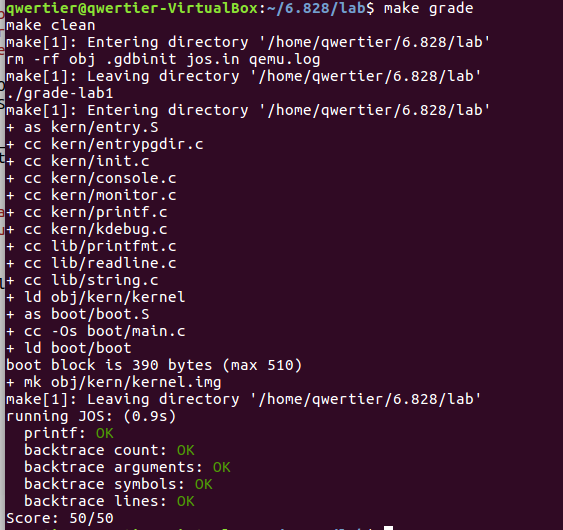
\includegraphics[width=6in]{figures/lab1/finish.png}
  \caption{实验1完成图}\label{fig:lab1:finish}
\end{figure}

\end{ExerciseList}


\begin{ExerciseList}
  \setcounter{Exercise}{0}
%% \begin{figure}[H]
%%   \centering
%%   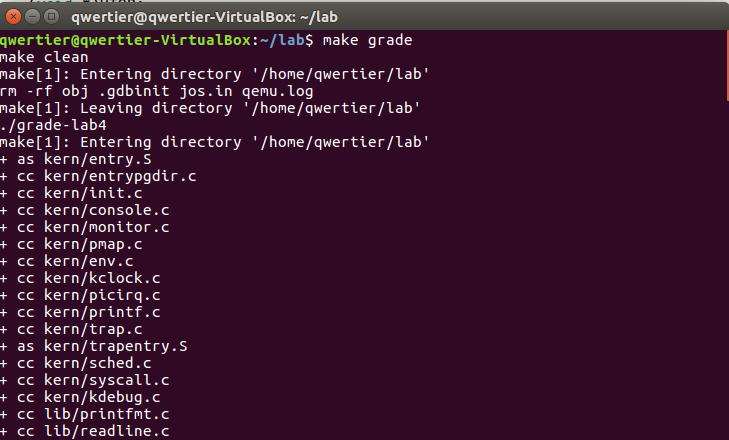
\includegraphics[width=6in]{figures/lab4/finish1.png}
%%   \caption{Lab4完成图}\label{fig:lab4:finish1}
  %% \end{figure}
  \section{Lab 2: Memory Management}

  \subsection{实验目的}

  操作系统必须要追踪记录哪些内存区域是空闲的,哪些是被占用的。JOS内核是以页(page)为最小粒度来管理内存的,它使用MMU来映射,保护每一块被分配出去的内存。在这里你要具体编写一下物理内存页的分配子函数。它利用一个结构体PageInfo的链表来记录哪些页是空闲的,链表中每一个结点对应一个物理页。

  \subsection{实验内容}

  \Exercise{在文件 kern/pmap.c 中,你必须要完成以下几个子函数的代码boot\_alloc(); mem\_init();  page\_init();  page\_alloc();page\_free();}

  先来看mem\_init()的代码。

  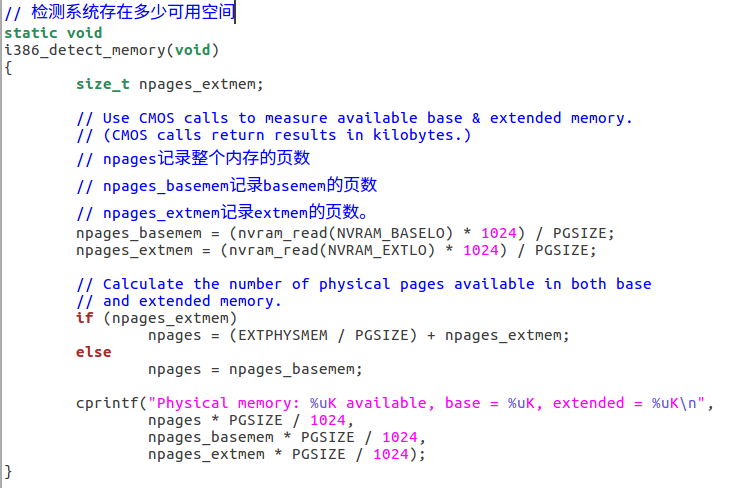
\includegraphics[width=6in]{figures/lab2/image40.png}

  这是i386\_detect\_memory 子函数的代码及注释。

  下面到了第一个需要添加的部分。

  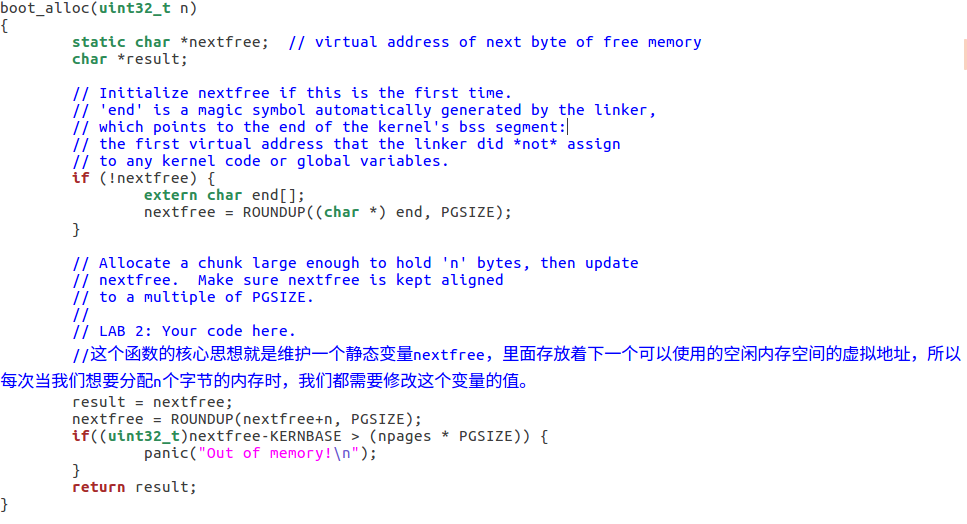
\includegraphics[width=6in]{figures/lab2/image41.png}

  Page\_init()需要补全的第二个函数。

  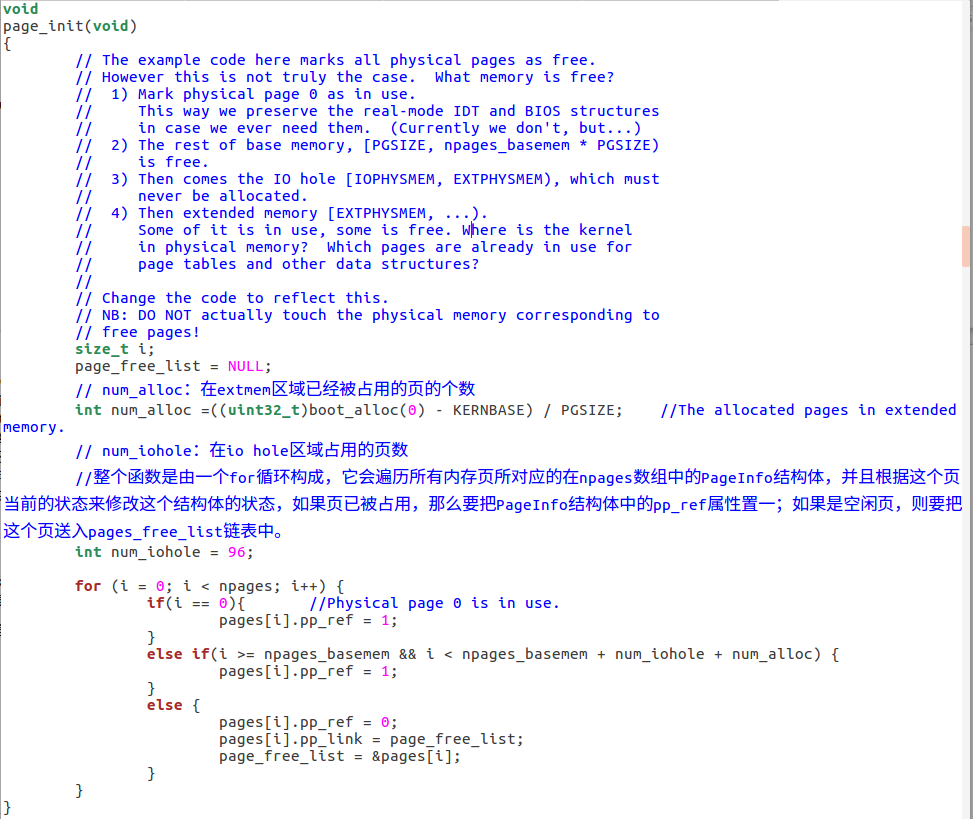
\includegraphics[width=6in]{figures/lab2/image42.png}

  接下来就是page\_alloc() 和page\_free()两个函数。

  先实现page\_alloc()函数,通过注释我们可以知道这个函数的功能就是分配一个物理页。而函数的返回值就是这个物理页所对应的PageInfo结构体。

  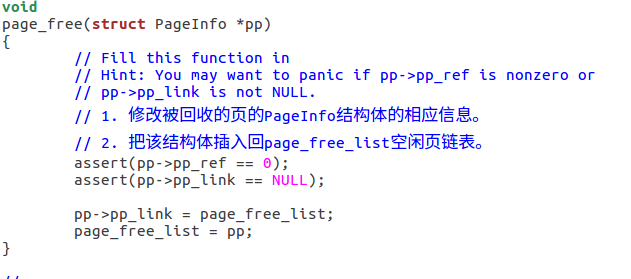
\includegraphics[width=6in]{figures/lab2/image44.png}

  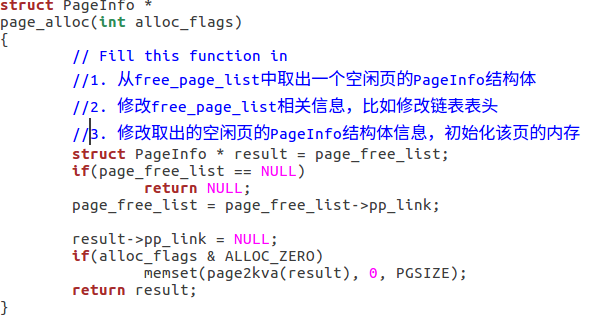
\includegraphics[width=6in]{figures/lab2/image43.png}

  实现page\_free()方法,根据注释可知,这个方法的功能就是把一个页的PageInfo结构体再返回给page\_free\_list空闲页链表,代表回收了这个页。

  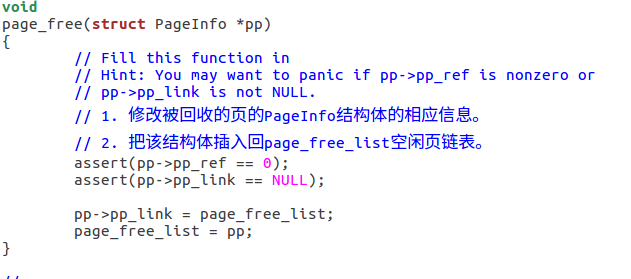
\includegraphics[width=6in]{figures/lab2/image44.png}

  一个虚拟地址(Virtual Address)是由两部分组成,一个是段选择子(segment selector),另一个是段内偏移(segment offset)。一个线性地址(Linear Address)指的是通过段地址转换机构把虚拟地址进行转换之后得到的地址。一个物理地址(Physical Addresses)是分页地址转换机构把线性地址进行转换之后得到的真实的内存地址,这个地址将会最终送到你的内存芯片的地址总线上。

  xp/Nx paddr – 查看paddr物理地址处开始的,N个字的16进制的表示结果。

  info registers – 展示所有内部寄存器的状态。

  info mem – 展示所有已经被页表映射的虚拟地址空间,以及它们的访问优先级。

  info pg – 展示当前页表的结构。

  \Exercise{参阅“ 英特尔80386参考手册”的第5章和第6章 ,如果还没有这样做的话。仔细阅读关于页面翻译和页面保护的章节(5.2和6.4)。浏览有关细分的部分; 而JOS使用分页硬件进行虚拟内存和保护时,在x86上不能禁用段转换和基于段的保护,因此需要对其进行基本的了解。}

  \Exercise{了解QEMU的一些指令,查看内存。}

  \Exercise{完成pgdir\_walk()boot\_map\_region()page\_lookup()   page\_remove()page\_insert()}

  函数给定一个页目录表指针 pgdir ,该函数应该返回线性地址va所对应的页表项指针。

  代码截图如下:


  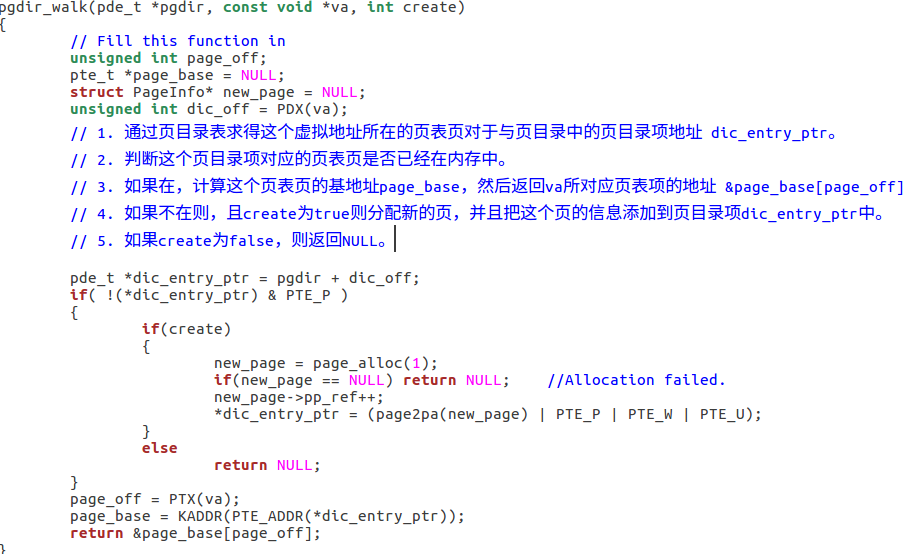
\includegraphics[width=6in]{figures/lab2/image45.png}


  boot\_map\_region函数,把虚拟地址空间范围[va, va+size)映射到物理空间[pa, pa+size)的映射关系加入到页表pgdir中。这个函数主要的目的是为了设置虚拟地址UTOP之上的地址范围,这一部分的地址映射是静态的,在操作系统的运行过程中不会改变,所以这个页的PageInfo结构体中的pp\_ref域的值不会发生改变。


      代码截图:


      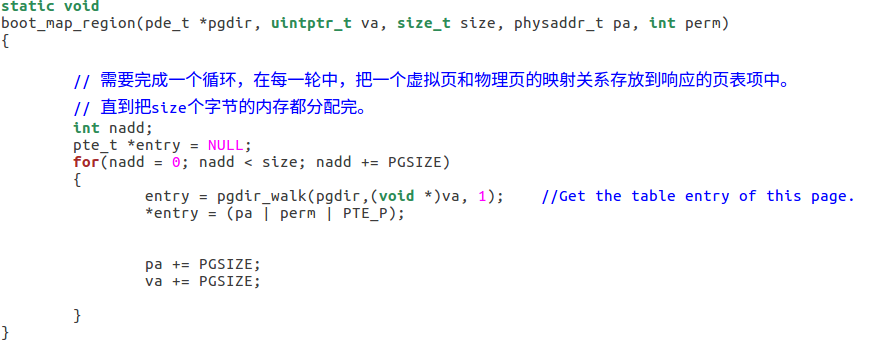
\includegraphics[width=6in]{figures/lab2/image46.png}


      page\_insert()功能上是完成:把一个物理内存中页pp与虚拟地址va建立映射关系。


      
\includegraphics[width=6in]{figures/lab2/image47.png}

      pp->pp\_ref++这条语句,一定要放在page\_remove之前。

      接下来继续完成page\_lookup()函数,返回虚拟地址va所映射的物理页的PageInfo结构体的指针,如果pte\_store参数不为0,则把这个物理页的页表项地址存放在pte\_store中。


      
\includegraphics[width=6in]{figures/lab2/image48.png}

      page\_remove函数,功能就是把虚拟地址va和物理页的映射关系删除。

      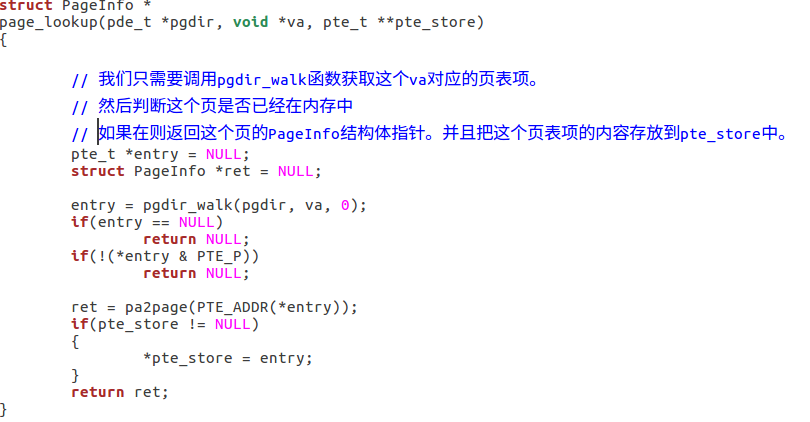
\includegraphics[width=6in]{figures/lab2/image49.png}

  由于内核和用户进程只能访问各自的地址空间,所以我们必须在x86页表中使用访问权限位(Permission Bits)来使用户进程的代码只能访问用户地址空间,而不是内核地址空间。否则用户代码中的一些错误可能会覆写内核中的数据,最终导致内核的崩溃。处在用户地址空间中的代码不能访问高于ULIM的地址空间,但是内核可以读写这部分空间。而内核和用户对于地址范围[UTOP, ULIM]有着相同的访问权限,那就是可以读取但是不可以写入。这一个部分的地址空间通常被用于把一些只读的内核数据结构暴露给用户地址空间的代码。在UTOP之下的地址范围是给用户进程使用的,用户进程可以访问,修改这部分地址空间的内容。

  \Exercise{剩下的工作就是要完善mem\_init()函数,现在要完善的功能就是把关于操作系统的一些重要的地址范围映射到现在的新页目录项上kern\_pgdir上。这里我们可以利用前面定义过的boot\_map\_region函数。}






\end{ExerciseList}


\begin{ExerciseList}

  \setcounter{Exercise}{0}
  \section{Lab 3: User Environments}

  \subsection{实验目的}

  在这个实验中,我们将实现操作系统的一些基本功能,来实现用户环境下的进程的正常运行。你将会加强JOS内核的功能,为它增添一些重要的数据结构,用来记录用户进程环境的一些信息;创建一个单一的用户环境,并且加载一个程序运行它。你也可以让JOS内核能够完成用户环境所作出的任何系统调用,以及处理用户环境产生的各种异常。

  \subsection{实验内容}

这个实验 多了很多代码

\begin{itemize}
\item INC/env.h	用户模式环境的公共定义
\item trap.h	陷阱处理的公共定义
\item syscall.h	从用户环境到内核的系统调用的公共定义
\item lib.h	用户模式支持库的公共定义
\item kern/env.h	用户模式环境的内核专用定义
\item env.c	内核代码实现用户模式环境
\item trap.h	内核专用陷阱处理定义
\item trap.c	陷阱处理代码
\item trapentry.S	汇编语言陷阱处理程序入口点
\item syscall.h	系统调用处理的内核专用定义
\item syscall.c	系统调用实现代码
\item Lib/Makefrag	Makefile片段构建用户模式库 obj / lib / libjos.a
\item entry.S中	用户环境的汇编语言入口
\item libmain.c	来自entry.S的用户模式库设置代码
\item syscall.c	用户模式系统调用存根函数
\item console.c中	putchar和getchar的用户模式实现,控制台I / O
\item exit.c中	用户模式执行的退出
\item panic.c	用户模式执行 panic
\item user/\*	各种测试程序来检查内核实验3代码
\end{itemize}

操作系统维护了三个重要的全局变量

\begin{minted}{C}
  struct Env *envs = NULL;//所有的 Env 结构体
  struct Env *curenv = NULL; //目前正在运行的用户环境
  static struct Env *env_free_list;
  //还没有被使用的 Env 结构体链表
\end{minted}

内核刚启动的时候,curenv的值为NULL。

具体Env 结构体定义:

  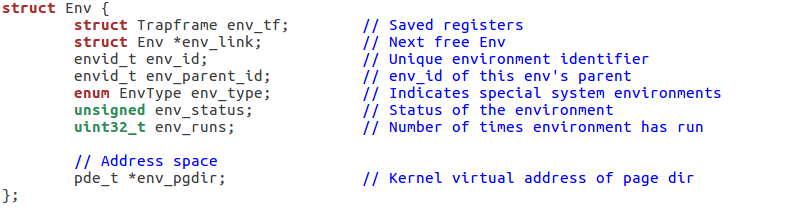
\includegraphics[width=6in]{figures/lab2/image52.png}


\begin{itemize}
  \item env\_tf:\\
      这个类型的结构体在inc/trap.h文件中被定义,里面存放着当用户环境暂停运行时,所有重要寄存器的值。内核也会在系统从用户态切换到内核态时保存这些值,这样的话用户环境可以在之后被恢复,继续执行。
  \item env\_link:\\
      这个指针指向在env\_free\_list中,该结构体的后一个free的Env结构体。当然前提是这个结构体还没有被分配给任意一个用户环境时,该域才有用。
  \item env\_id:\\
      这个值可以唯一的确定使用这个结构体的用户环境是什么。当这个用户环境终止,内核会把这个结构体分配给另外一个不同的环境,这个新的环境会有不同的env\_id值。
  \item env\_parent\_id:\\
    创建这个用户环境的父用户环境的env\_id
  \item env\_type:\\
    用于区别出来某个特定的用户环境。对于大多数环境来说,它的值都是 ENV\_TYPE\_USER.
  \item env\_status:\\
    这个变量存放以下可能的值
  \item ENV\_FREE:\\
    代表这个结构体是不活跃的,应该在链表env\_free\_list中。
  \item ENV\_RUNNABLE: \\
    代表这个结构体对应的用户环境已经就绪,等待被分配处理机。
  \item ENV\_RUNNING:\\
    代表这个结构体对应的用户环境正在运行。
  \item ENV\_NOT\_RUNNABLE: \\
    代表这个结构体所代表的是一个活跃的用户环境,但是它不能被调度运行,因为它在等待其他环境传递给它的消息。
  \item ENV\_DYING: \\
    代表这个结构体对应的是一个僵尸环境。一个僵尸环境在下一次陷入内核时会被释放回收。
  \item env\_pgdir:\\
    这个变量存放着这个环境的页目录的虚拟地址
\end{itemize}

\Exercise{现在你需要进一步去修改mem\_init()函数,来分配一个Env结构体数组,叫做envs。}

这个实验在做了lab2的实验之后就很好做了。

  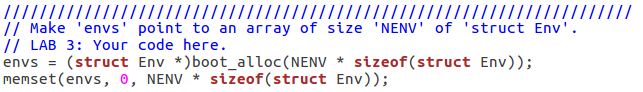
\includegraphics[width=6in]{figures/lab2/image53.png}

我们现在需要来运行一个用户环境,我们需要把内核设置成能够加载内核中的静态二进制文件。


\Exercise{region\_alloc(): 为用户环境分配物理地址空间}

   load\_icode(): 分析一个ELF文件,类似于boot loader做的那样,我们可以把它的内容加载到用户环境下。

   env\_create(): 利用env\_alloc函数和load\_icode函数,加载一个ELF文件到用户环境中

   env\_run(): 在用户模式下,开始运行一个用户环境。

  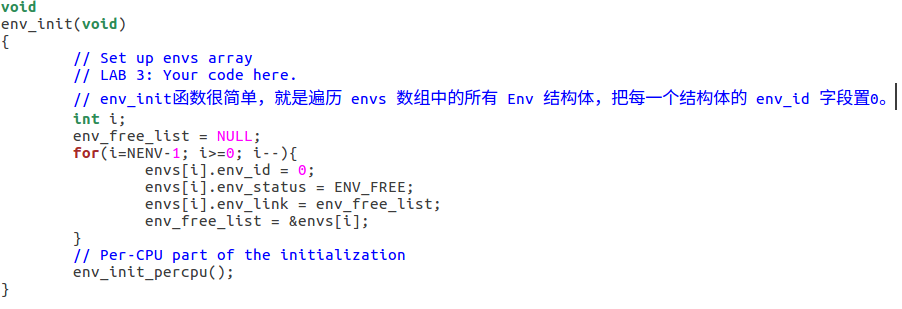
\includegraphics[width=6in]{figures/lab2/image54.png}

这是env\_init():初始化所有的在envs数组中的 Env结构体,并把它们加入到 env\_free\_list中。 还要调用 env\_init\_percpu,这个函数要配置段式内存管理系统,让它所管理的段,可能具有两种访问优先级其中的一种,一个是内核运行时的0优先级,以及用户运行时的3优先级。

 env\_setup\_vm(): 为一个新的用户环境分配一个页目录表,并且初始化这个用户环境的地址空间中的和内核相关的部分。

  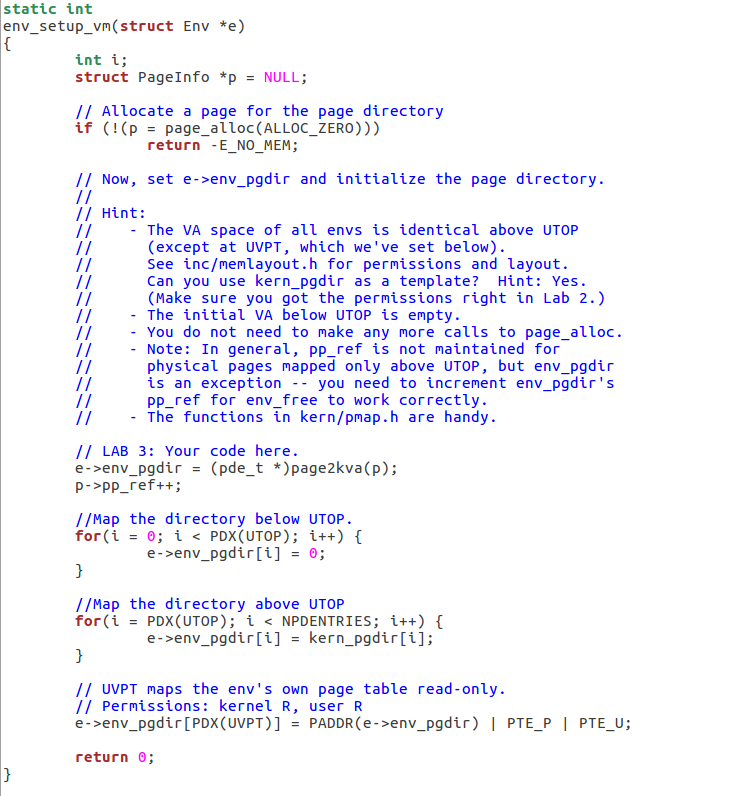
\includegraphics[width=6in]{figures/lab2/image55.png}

  region\_alloc 为用户环境分配物理空间,这里注意我们要先把起始地址和终止地址进行页对齐,对其之后我们就可以以页为单位,为其一个页一个页的分配内存,并且修改页目录表和页表。

  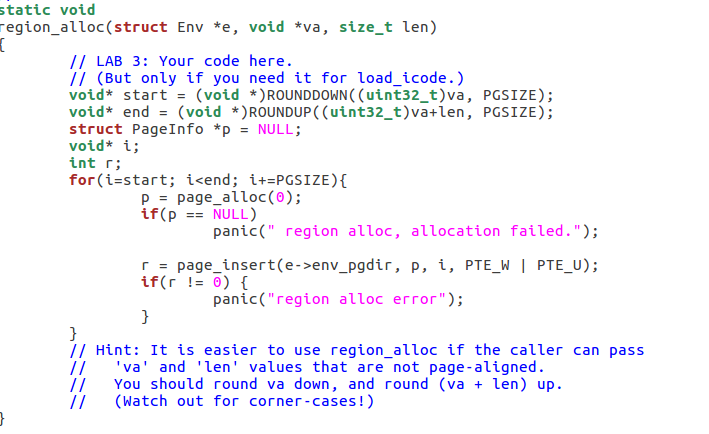
\includegraphics[width=6in]{figures/lab2/image56.png}

  load\_icode 功能是为每一个用户进程设置它的初始代码区,堆栈以及处理器标识位。每个用户程序都是ELF文件,所以我们要解析该ELF文件。

  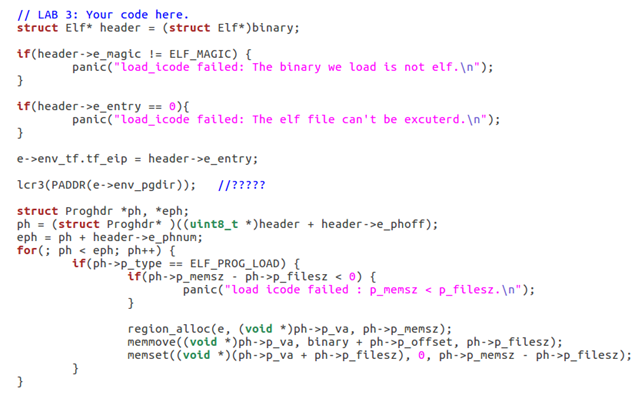
\includegraphics[width=6in]{figures/lab2/image57.png}

  env\_create 是利用env\_alloc函数和load\_icode函数,加载一个ELF文件到用户环境中。

  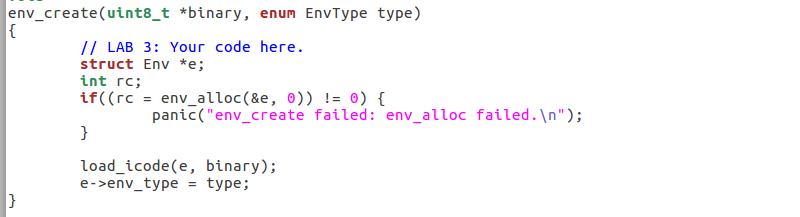
\includegraphics[width=6in]{figures/lab2/image58.png}

  env\_run 是真正开始运行一个用户环境

  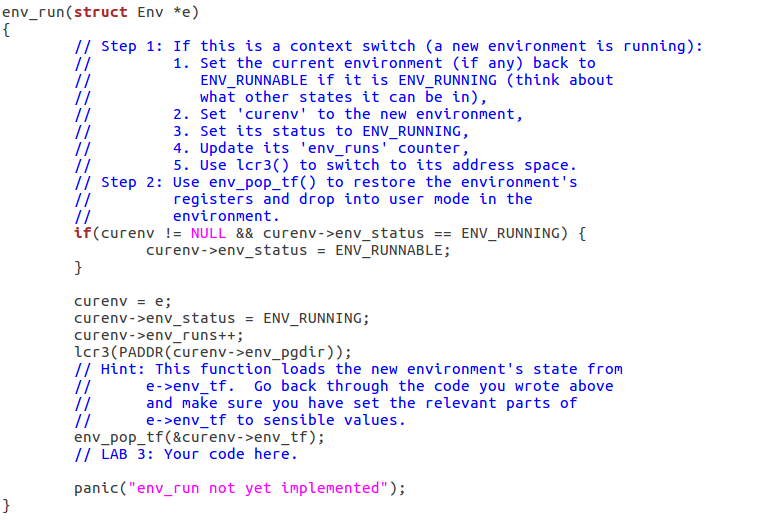
\includegraphics[width=6in]{figures/lab2/image59.png}

  用户环境的代码被调用前,操作系统一共按顺序执行了以下几个函数:

  * start (kern/entry.S)

  * i386\_init (kern/init.c)

  cons\_init

  mem\_init

  env\_init

  trap\_init (目前还未实现)

  env\_create

  env\_run

  env\_pop\_tf

显然用户级线程是不可以调用系统内存的,因为现在系统无法从用户态切换到内核态。所以你需要实现一个基本的异常/系统调用处理机制,使得内核可以从用户态转换为内核态。

\begin{enumerate}
\item 中断向量表:\\
     处理器保证中断和异常只能够引起内核进入到一些特定的,被事先定义好的程序入口点,而不是由触发中断的程序来决定中断程序入口点。\\
     X86允许多达256个不同的中断和异常,每一个都配备一个独一无二的中断向量。一个向量指的就是0到255中的一个数。一个中断向量的值是根据中断源来决定的:不同设备,错误条件,以及对内核的请求都会产生出不同的中断和中断向量的组合。CPU将使用这个向量作为这个中断在中断向量表中的索引,这个表是由内核设置的,放在内核空间中,和GDT很像。通过这个表中的任意一个表项,处理器可以知道:\\
   *需要加载到EIP寄存器中的值,这个值指向了处理这个中断的中断处理程序的位置。\\
   *需要加载到CS寄存器中的值,里面还包含了这个中断处理程序的运行特权级。(即这个程序是在用户态还是内核态下运行。)\\
\item 任务状态段\\
   处理器还需要一个地方来存放,当异常/中断发生时,处理器的状态,比如EIP和CS寄存器的值。这样的话,中断处理程序一会可以重新返回到原来的程序中。这段内存自然也要保护起来,不能被用户态的程序所篡改。\\
   正因为如此,当一个x86处理器要处理一个中断,异常并且使运行特权级从用户态转为内核态时,它也会把它的堆栈切换到内核空间中。一个叫做 “任务状态段(TSS)”的数据结构将会详细记录这个堆栈所在的段的段描述符和地址。处理器会把SS,ESP,EFLAGS,CS,EIP以及一个可选错误码等等这些值压入到这个堆栈上。然后加载中断处理程序的CS,EIP值,并且设置ESP,SS寄存器指向新的堆栈。\\
    尽管TSS非常大,并且还有很多其他的功能,但是JOS仅仅使用它来定义处理器从用户态转向内核态所采用的内核堆栈,由于JOS中的内核态指的就是特权级0,所以处理器用TSS中的ESP0,SS0字段来指明这个内核堆栈的位置,大小。
\end{enumerate}

\textbf{扩展0-31号中断}

\begin{enumerate}
\item trap\_init() 先将所有中断处理函数的起始地址放到中断向量表IDT中。

   \item 当中断发生时,不管是外部中断还是内部中断,处理器捕捉到该中断,进入核心态,根据中断向量去查询中断向量表,找到对应的表项
  \item 保存被中断的程序的上下文到内核堆栈中,调用这个表项中指明的中断处理函数。
  \item 执行中断处理函数。
\item 执行完成后,恢复被中断的进程的上下文,返回用户态,继续运行这个进程。
\item	阅读 第9章异常和中断 的 80386程序员手册 (或第5章 IA-32开发者手册)
\end{enumerate}

\Exercise{编辑一下trapentry.S 和 trap.c 文件,并且实现上面所说的功能。宏定义 TRAPHANDLER 和 TRAPHANDLER\_NOEC 会对你有帮助。你将会在 trapentry.S文件中为在inc/trap.h文件中的每一个trap加入一个入口指, 你也将会提供\_alttraps的值。}

需要修改trap\_init()函数来初始化idt表,使表中每一项指向定义在trapentry.S中的入口指针,SETGATE宏定义在这里用得上。

你所实现的 \_alltraps 应该:

\begin{enumerate}
\item 把值压入堆栈使堆栈看起来像一个结构体 Trapframe
\item 加载 GD\_KD 的值到 %ds, %es寄存器中
\item 把\%esp的值压入,并且传递一个指向Trapframe的指针到trap()函数中。
\item 调用trap trapentry.S
\end{enumerate}

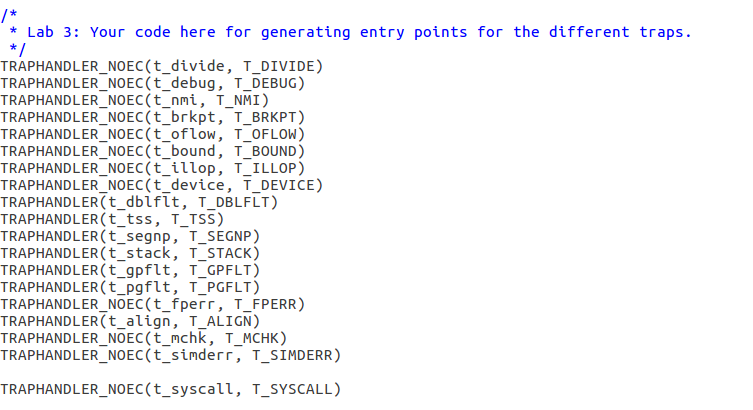
\includegraphics[width=6in]{figures/lab2/image62.png}

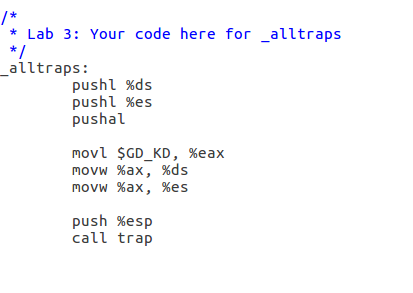
\includegraphics[width=6in]{figures/lab2/image61.png}

对于trap\_init定义如下:

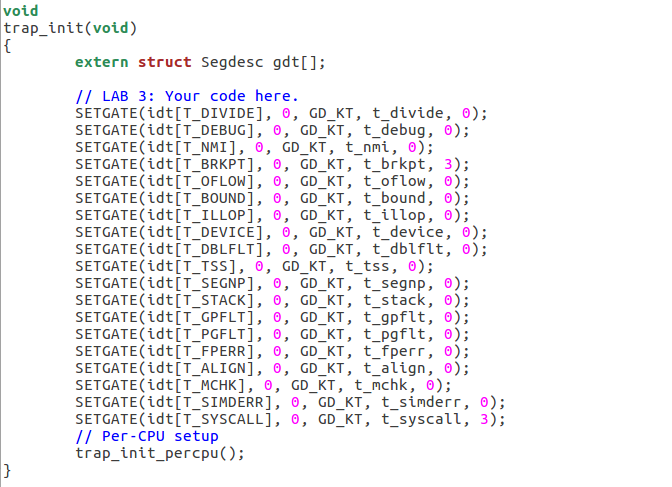
\includegraphics[width=6in]{figures/lab2/image63.png}

  \Exercise{这个练习和上一个基本类似}

  断点异常,异常号为3,这个异常可以让调试器能够给程序加上断点。加断点的基本原理就是把要加断点的语句用一个 INT3 指令替换,执行到INT3时,会触发软中断。在JOS中,我们将通过把这个异常转换成一个伪系统调用,这样的话任何用户环境都可以使用这个伪系统调用来触发JOS kernel monitor。

  问答:在上面的break point exception测试程序中,如果你在设置IDT时,对break point exception采用不同的方式进行设置,可能会产生触发不同的异常,有可能是break point exception,有可能是 general protection exception。这是为什么?你应该怎么做才能得到一个我们想要的breakpoint exception,而不是general protection exception?

  答:通过实验发现出现这个现象的问题就是在设置IDT表中的breakpoint exception的表项时,如果我们把表项中的DPL字段设置为3,则会触发break point exception,如果设置为0,则会触发general protection exception。DPL字段代表的含义是段描述符优先级(Descriptor Privileged Level),如果我们想要当前执行的程序能够跳转到这个描述符所指向的程序哪里继续执行的话,有个要求,就是要求当前运行程序的CPL,RPL的最大值需要小于等于DPL,否则就会出现优先级低的代码试图去访问优先级高的代码的情况,就会触发general protection exception。那么我们的测试程序首先运行于用户态,它的CPL为3,当异常发生时,它希望去执行 int 3指令,这是一个系统级别的指令,用户态命令的CPL一定大于 int 3 的DPL,所以就会触发general protection exception,但是如果把IDT这个表项的DPL设置为3时,就不会出现这样的现象了,这时如果再出现异常,肯定是因为我们还没有编写处理break point exception的程序所引起的,所以是break point exception。

  \Exercise{给中断向量T\_SYSCALL编写一个中断处理函数。你需要去编辑kern/trapentry.S和kern/trap.c中的trap\_init()函数。你也需要去修改trap\_dispatch()函数,使他能够通过调用syscall()(在kern/syscall.c中定义的)函数处理系统调用中断。最终你需要去实现kern/syscall.c中的syscall()函数。确保这个函数会在系统调用号为非法值时返回-E\_INVAL。你应该充分理解lib/syscall.c文件。我们要处理在inc/syscall.h文件中定义的所有系统调用。}

  我们需要了解一下系统调用的整个流程,如果现在运行的是内核态的程序的话,此时调用了一个系统调用,比如 sys\_cputs 函数时,此时不会触发中断,那么系统会直接执行定义在 lib/syscall.c 文件中的 sys\_cputs,我们可以看一下这个文件,可以发现这个文件中定义了几个比较常用的系统调用,包括 sys\_cputs, sys\_cgetc 等等。我们还会发现他们都是统一调用一个 syscall 函数,通过这个函数的代码发现其实它是执行了一个汇编指令。所以最终是这个函数完成了系统调用。以上是运行在内核态下的程序,调用系统调用时的流程。但是如果是用户态程序呢?这个练习就是让我们编写程序使我们的用户程序在调用系统调用时,最终也能经过一系列的处理最终去执行 lib/syscall.c 中的 syscall 指令。让我们看一下这个过程,当用户程序中要调用系统调用时,比如 sys\_cputs,从它的汇编代码中我们会发现,它会执行一个 int \$0x30 指令,这个指令就是软件中断指令,这个中断的中断号就是 0x30,即 T\_SYSCALL,所以题目中让我们首先为这个中断号编写一个中断处理函数,我们首先就要在 kern/trapentry.S 文件中为它声明它的中断处理函数,即TRAPHANDLER\_NOEC,就像我们为其他中断号所做的那样。

  所以我们可以假象一下,是不是 kern/syscall.c 中的 syscall 就是一个外壳函数,它的存在就是为了能够调用 lib/syscall 的呢? 所以我们按照这个思路继续进行下去,我们再继续观察 kern/syscall.c 中的其他函数,会惊人的发现,kern/syscall.c 中的所有函数居然和 lib/syscall.c 中的所有函数都是一样的!!比如 在这两个文件中都有 sys\_cputs 函数,但是我们仔细观察可以发现这两个同名的函数,实现方式却不一样。

  其实系统调用,syscall函数需要处理各种函数的信息

  \Exercise{用户程序真正开始运行的地方是在lib/entry.S文件中。该文件中,首先会进行一些设置,然后就会调用lib/libmain.c 文件中的 libmain() 函数。你首先要修改一下 libmain() 函数,使它能够初始化全局指针 thisenv ,让它指向当前用户环境的 Env 结构体。}

  然后 libmain() 函数就会调用 umain,这个 umain 程序恰好是 user/hello.c 中被调用的函数。在之前的实验中我们发现,hello.c程序只会打印 "hello, world" 这句话,然后就会报出 page fault 异常,原因就是 thisenv->env\_id 这条语句。现在你已经正确初始化了这个 thisenv的值,再次运行就应该不会报错了。

  其实这个练习就是让你通过程序获得当前正在运行的用户环境的 env\_id , 以及这个用户环境所对应的 Env 结构体的指针。 env\_id 我们可以通过调用 sys\_getenvid() 这个函数来获得。那么如何获得它对应的 Env结构体指针呢?

  通过阅读 lib/env.h 文件我们知道,env\_id的值包含三部分,第31位被固定为0;第10~30这21位是标识符,标示这个用户环境;第0~9位代表这个用户环境所采用的 Env 结构体,在envs数组中的索引。所以我们只需知道 env\_id 的低 0~9 位,我们就可以获得这个用户环境对应的 Env 结构体了。

\Exercise{内存保护是操作系统的非常重要的一项功能,它可以防止由于用户程序崩溃对操作系统带来的破坏与影响。操作系统通常依赖于硬件的支持来实现内存保护。操作系统可以让硬件能够始终知晓哪些虚拟地址是有效的,哪些是无效的。当程序尝试去访问一个无效地址,或者尝试去访问一个超出它访问权限的地址时,处理器会在这个指令处终止,并且触发异常,陷入内核态,与此同时把错误的信息报告给内核。如果这个异常是可以被修复的,那么内核会修复这个异常,然后程序继续运行。如果异常无法被修复,则程序永远不会继续运行。}

 作为一个可修复异常的例子,让我们考虑一下可自动扩展的堆栈。在许多系统中,内核在初始情况下只会分配一个内核堆栈页,如果程序想要访问这个内核堆栈页之外的堆栈空间的话,就会触发异常,此时内核会自动再分配一些页给这个程序,程序就可以继续运行了。

 系统调用也为内存保护带来了问题。大部分系统调用接口让用户程序传递一个指针参数给内核。这些指针指向的是用户缓冲区。通过这种方式,系统调用在执行时就可以解引用这些指针。但是这里有两个问题:

 1. 在内核中的page fault要比在用户程序中的page fault更严重。如果内核在操作自己的数据结构时出现 page faults,这是一个内核的bug,而且异常处理程序会中断整个内核。但是当内核在解引用由用户程序传递来的指针时,它需要一种方法去记录此时出现的任何page faults都是由用户程序带来的。

 2. 内核通常比用户程序有着更高的内存访问权限。用户程序很有可能要传递一个指针给系统调用,这个指针指向的内存区域是内核可以进行读写的,但是用户程序不能。此时内核必须小心不要去解析这个指针,否则的话内核的重要信息很有可能被泄露。

  现在你需要通过仔细检查所有由用户传递来指针所指向的空间来解决上述两个问题。当一个程序传递给内核一个指针时,内核会检查这个地址是在整个地址空间的用户地址空间部分,而且页表也运行进行内存的操作。

修改kern/trap.c文件,使其能够实现:当在内核模式下发现页错,trap.c 文件会panic。

提示:

为了能够判断这个page fault是出现在内核模式下还是用户模式下,我们应该检查 tf\_cs 的低几位。

阅读 user\_mem\_assert (在 kern/pmap.c),并且实现 user\_mem\_check;

修改一下 kern/syscall.c 去检查输入参数。

启动内核后,运行 user/buggyhello 程序,用户环境可以被销毁,内核不可以panic,你应该看到:

[00001000] user\_mem\_check assertion failure for va 00000001

[00001000] free env 00001000

Destroyed the only environment - nothing more to do!

首先我们应该根据什么来判断当前运行的程序时处在内核态下还是用户态下?答案是根据 CS 段寄存器的低2位,这两位的名称叫做 CPL 位,表示当前运行的代码的访问权限级别,0代表是内核态,3代表是用户态。

题目要求我们在检测到这个 page fault 是出现在内核态时,要把这个事件 panic 出来,所以我们把 page\_fault\_handler 文件修改如下:

user\_mem\_check 函数的功能是检查一下当前用户态程序是否有对虚拟地址空间 [va, va+len] 的 perm| PTE\_P 访问权限。自然我们要做的事情应该是,先找到这个虚拟地址范围对应于当前用户态程序的页表中的页表项,然后再去看一下这个页表项中有关访问权限的字段,是否包含 perm | PTE\_P,只要有一个页表项是不包含的,就代表程序对这个范围的虚拟地址没有 perm|PTE\_P 的访问权限。以上就是这段代码的大致思想。

其中syscall中的sys\_cputs函数,这个函数对虚拟地址检查权限。

运行后可以看到

\Exercise{没有新东西,就是测试练习9的代码}

\end{ExerciseList}


\section{Lab 4: Preemptive Multitasking}

\subsection{实验简介}

在本实验中,你将会实现抢占式多进程管理。需要哈工大操作系统课第五章的知识。

在第一部分里,需要向JOS添加多核支持,实现转轮调度,并添加基础的系统调用(用于添加或删除运行上下文环境,申请或对应内存)。

在第二部分里,需要实现Unix风格的fork()函数,支持从用户态环境建立一个自己的拷贝。

最后在第三部分里,需要添加对进程间通信(IPC)的支持,允许不同的用户态环境减间的交流并同步。还需要添加对硬件时钟中断和抢占的支持。

\subsection{实验目的}

\begin{itemize}
\item 了解并实现抢占式多进程管理
\item 了解并实现转轮法调度算法
\end{itemize}

\subsection{实验内容}

\subsubsection{准备工作}

需要用git commit把Lab3的成果提交,然后在lab3分支上新建分支lab4,并合并远程分支lab4。

\begin{figure}[H]
  \centering
  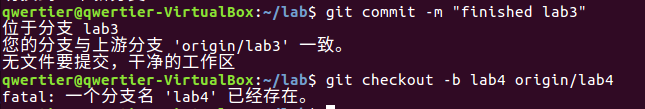
\includegraphics[width=6in]{figures/lab4/git_commit.png}
  \caption{使用git的截图}\label{fig:lab1:git_commit}
\end{figure}

\begin{ExerciseList}

\setcounter{Exercise}{0}

\subsubsection[第一部分: 多处理器支持及协作式多任务]{第一部分: 多处理器支持\footnote{Multiprocessor Support}及协作式多任务\footnote{Cooperative Multitasking} }

协作式多进程(Cooperative)指的是:进程主动(定期或者空闲时候)让出CPU的执行时间给其他进程来执行,这种模式非常依赖于程序的设计,如果程序写的很差, 进程长时间占用CPU的执行时间(大量计算密集型的操作或者等待外设等),这会让其他进程没有机会执行,从而造成整个操作系统失去响应。

协作式多任务在早期的操作系统中使用得比较广泛(比如Windows 9x、Classic Mac OS等等)。

我们将使JOS支持“对称多处理”(SMP),这是一种多处理器模型,其中所有的CPU都可以访问系统资源,例如内存和I / O总线。虽然所有的CPU在功能上与SMP完全相同,但在引导过程中,它们可以分为两种类型:引导处理器(BSP)负责初始化系统和引导操作系统; 并且只有在操作系统启动并运行之后,应用处理器(AP)才由BSP激活。BSP的处理器是由硬件和BIOS决定的。到目前为止,所有现有的JOS代码已经在BSP上运行。

在SMP系统中,每个CPU都有一个附带的本地APIC(LAPIC)单元。LAPIC单元负责在整个系统中提供中断。LAPIC还为连接的CPU提供唯一的标识符。在这个实验中,我们利用了LAPIC单元的下列基本功能(在kern / lapic.c中):

\begin{itemize}
\item 读取LAPIC标识符(APIC ID),以告知我们的代码当前正在哪个CPU上运行(请参阅cpunum())。
\item 发送STARTUP从BSP到的AP间中断(IPI)带来的其他CPU。
\item 在C部分,我们编程LAPIC的内置定时器来触发时钟中断,以支持抢先式多任务处理(请参阅参考资料 apic\_init())。
\end{itemize}

\Exercise{实现kern/pmap.c文件中的mmio\_map\_region函数。想要看它是如何被用到的,需要看kern/lapic.c中的lapic\_init。}

\begin{minted}{C}
void *
mmio_map_region(physaddr_t pa, size_t size)
{
    // Where to start the next region.  Initially, this is the
    // beginning of the MMIO region.  Because this is static, its
    // (just like nextfree in boot_alloc).
    static uintptr_t base = MMIOBASE;

    // Reserve size bytes of virtual memory starting at base and
    // map physical pages [pa,pa+size) to virtual addresses
    // [base,base+size).  Since this is device memory and not
    // regular DRAM, you'll have to tell the CPU that it isn't
    // safe to cache access to this memory.  Luckily, the page
    // tables provide bits for this purpose; simply create the
    // mapping with PTE_PCD|PTE_PWT (cache-disable and
    // write-through) in addition to PTE_W.  (If you're interested
    // in more details on this, see section 10.5 of IA32 volume
    // 3A.)
    //
    // Be sure to round size up to a multiple of PGSIZE and to
    // handle if this reservation would overflow MMIOLIM (it's
    // okay to simply panic if this happens).
    //
    // Hint: The staff solution uses boot_map_region.
    //
    // Your code here:
    int nextbase = ROUNDUP(base + size, PGSIZE);
    if (nextbase >= MMIOLIM) {
            panic("nextbase >= MMIOLIM");
    }
    boot_map_region(kern_pgdir, base, size, pa, PTE_PCD | PTE_PWT | PTE_W);

    void *ret = (void *)base;
    base = nextbase;

    return ret;
    // panic("mmio_map_region not implemented");
}
\end{minted}

在启动AP之前,BSP应首先收集有关多处理器系统的信息,例如CPU的总数,APIC ID和LAPIC单元的MMIO地址。kern / mpconfig.c中的mp\_init()函数 通过读取驻留在BIOS的内存区域中的MP配置表来检索此信息。

\Exercise{阅读kern/init.c中的boot\_aps()和mp\_main()函数,以及kern/mpentry.S文件。确保你理解了AP启动时的控制流。修改你在kern/pmap.c中的page\_init()的实现来防止添加MPENTRY\_PADDR位置的页到free list,以让我们可以安全的拷贝并在那个物理地址执行AP运行代码。你的代码应该通过check\_page\_free\_list()测试,但是可能通不过check\_kern\_pgdir()测试,这个我们稍后会修正。}

\begin{minted}{C}
// Setup code for APs
void
mp_main(void)
{
    // We are in high EIP now, safe to switch to kern_pgdir
    lcr3(PADDR(kern_pgdir));
    cprintf("SMP: CPU %d starting\n", cpunum());

    lapic_init();
    env_init_percpu();
    trap_init_percpu();
    xchg(&thiscpu->cpu_status, CPU_STARTED); // tell boot_aps() we're up

    // Now that we have finished some basic setup, call sched_yield()
    // to start running processes on this CPU.  But make sure that
    // only one CPU can enter the scheduler at a time!
    //
    // Your code here:

    lock_kernel();  // 锁定内核
    sched_yield();  // 调用轮换调度算法

    // Remove this after you finish Exercise 4
    // for (;;);
}
\end{minted}

编写多处理器操作系统时,区分CPU私有状态\footnote{per-CPU state}以及全局状态\footnote{global state}。需要了解如下部分:

\begin{itemize}
\item CPU独立内核栈\footnote{Per-CPU kernel stack}
\item Per-CPU TSS(Task State Segment)和TSS描述符
\item Per-CPU 当前环境指针
\item Per-CPU 系统寄存器
\end{itemize}

\Exercise{修改kern/pmap.c中的mem\_init\_mp()函数,来映射在KSTACKTOP位置的CPU独立栈。每个栈大小是KSTKSIZE字节加上KSTKGAP字节。代码需要通过check\_kern\_pgdir()测试。}

\begin{minted}{C}
void
mem_init_mp(void)
{
    // Map per-CPU stacks starting at KSTACKTOP, for up to 'NCPU' CPUs.
    //
    // For CPU i, use the physical memory that 'percpu_kstacks[i]' refers
    // to as its kernel stack. CPU i's kernel stack grows down from virtual
    // address kstacktop_i = KSTACKTOP - i * (KSTKSIZE + KSTKGAP), and is
    // divided into two pieces, just like the single stack you set up in
    // mem_init:
    //     * [kstacktop_i - KSTKSIZE, kstacktop_i)
    //          -- backed by physical memory
    //     * [kstacktop_i - (KSTKSIZE + KSTKGAP), kstacktop_i - KSTKSIZE)
    //          -- not backed; so if the kernel overflows its stack,
    //             it will fault rather than overwrite another CPU's stack.
    //             Known as a "guard page".
    //     Permissions: kernel RW, user NONE
    //
    // LAB 4: Your code here:

    int i;
    for (i=0; i<NCPU; i++) {
        boot_map_region(kern_pgdir,
                KSTACKTOP - i * (KSTKSIZE + KSTKGAP) - KSTKSIZE,  // 起始地址
                KSTKSIZE,                                         // 内存块大小
                PADDR(percpu_kstacks[i]),
                PTE_W|PTE_P);
    }
}
\end{minted}

\Exercise{kern/trap.c文件中trap\_init\_percpu()的代码初始化了TSS和TSS描述符。在Lab3中可以正常工作,但是在其他CPU上运行时就会出问题。修改这些代码已让它能运行在所有CPU上。}

\begin{minted}{C}
void
trap_init_percpu(void)
{
        // The example code here sets up the Task State Segment (TSS) and
        // the TSS descriptor for CPU 0. But it is incorrect if we are
        // running on other CPUs because each CPU has its own kernel stack.
        // Fix the code so that it works for all CPUs.
        //
        // Hints:
        //   - The macro "thiscpu" always refers to the current CPU's
        //     struct CpuInfo;
        //   - The ID of the current CPU is given by cpunum() or
        //     thiscpu->cpu_id;
        //   - Use "thiscpu->cpu_ts" as the TSS for the current CPU,
        //     rather than the global "ts" variable;
        //   - Use gdt[(GD_TSS0 >> 3) + i] for CPU i's TSS descriptor;
        //   - You mapped the per-CPU kernel stacks in mem_init_mp()
        //
        // ltr sets a 'busy' flag in the TSS selector, so if you
        // accidentally load the same TSS on more than one CPU, you'll
        // get a triple fault.  If you set up an individual CPU's TSS
        // wrong, you may not get a fault until you try to return from
        // user space on that CPU.
        //
        // LAB 4: Your code here:

        // Setup a TSS so that we get the right stack
        // when we trap to the kernel.
        thiscpu->cpu_ts.ts_esp0 = KSTACKTOP - cpunum() * (KSTKSIZE + KSTKGAP);
        thiscpu->cpu_ts.ts_ss0 = GD_KD;

        // Initialize the TSS slot of the gdt.
    gdt[(GD_TSS0 >> 3) + cpunum()] = SEG16(STS_T32A,
                                           (uint32_t) &thiscpu->cpu_ts,
                                           sizeof(struct Taskstate) - 1,
                                           0);
    gdt[(GD_TSS0 >> 3) + cpunum()].sd_s = 0;

        // Load the TSS selector (like other segment selectors, the
        // bottom three bits are special; we leave them 0)
        //ltr(GD_TSS0 + cpunum()*sizeof(struct Segdesc));
    ltr(((GD_TSS0 >> 3) + cpunum()) << 3);

        // Load the IDT
    lidt(&idt_pd);
}
\end{minted}

如图\ref{fig:lab4:mcpu},四个CPU都正常初始化。

\begin{figure}[H]
  \centering
  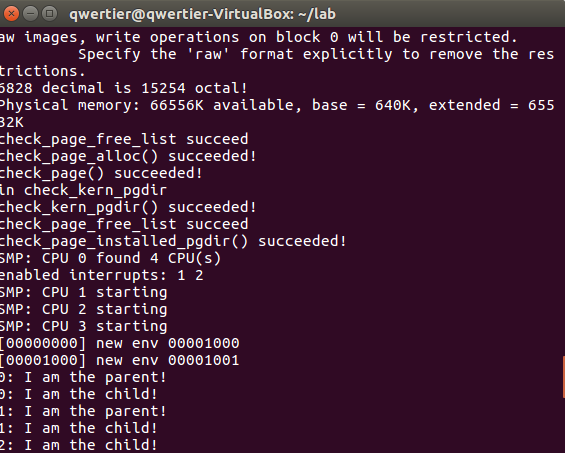
\includegraphics[width=6in]{figures/lab4/mcpu.png}
  \caption{QEMU启动截图}\label{fig:lab4:mcpu}
\end{figure}

我们当前的代码在mp\_main()函数中初始化AP之后就不会再运行了。在让AP继续运行前,我们首先需要解决竞争问题当多个CPU运行同一个内核时。最简单的方式是使用一个大内核锁。这个大内核锁是一个全局锁会作用于当进程进入内核模式时,而且在返回用户模式时会被释放。在这个模型下,用户模式下的进程可以在当前运行在任何可行的CPU上,但是不能有任何一个进程运行在内核模式中。

应该在四个位置应用大内核锁:

\begin{itemize}
\item 在i386\_init()BSP唤醒其他CPU之前获取锁。
\item 在mp\_main()初始化AP后获取锁,然后调用sched\_yield()该AP启动运行环境。
\item 在trap()从用户模式中获取锁时。要确定陷阱是发生在用户模式还是在内核模式下,请检查低位tf\_cs。
\item 在切换到用户模式之前env\_run(),立即释放锁定。不要太早或太晚,否则会遇到冲突。
\end{itemize}

\Exercise{如上所述,应用大内核锁,通过调用lock\_kernel()并unlock\_kernel()在适当的位置。}

只需要在i386\_init(), mp\_main(), trap()这几个函数中添加lock\_kernel(),在env\_run()中添加unlock\_kernel()即可。

因为前三个函数都是进入内核态,而最后的env\_run()是从内核态返回用户态。

\Exercise{在/kern/sched.c文件的sched\_yield()中实现轮转调度,不要忘记修改syscall()发送sys\_yield()。确保在mp\_main()中调用sched\_yield()。并修改kern/inic.c来创建所有运行程序user/yield.c。}

JOS的轮转调度算法如下:

\begin{enumerate}
\item 函数sched\_yield()在新的kern/sched.c中,负责选择一个进程来运行。envs[]以循环的方式按顺序搜索数组,在刚才运行的环境之后(或者在数组的开始处,如果没有以前运行的环境)开始,选择状态为ENV\_RUNNABLE(见inc/ env.h)的进程,并调用env\_run()进入该进程。
\item sched\_yield()决不能同时在两个CPU上运行相同的进程。它可以告诉一个环境当前正在某个CPU(可能是当前的CPU)上运行,因为该进程的状态将会是ENV\_RUNNING。
\item 已经实现了一个新的系统调用sys\_yield(),进程可以调用内核的sched\_yield()功能,从而自动放弃CPU到不同的进程。
\end{enumerate}

修改kern/sched.c的sched\_yield()函数:

\begin{minted}{C}
void
sched_yield(void)
{
        struct Env *idle;

        // Implement simple round-robin scheduling.
        //
        // Search through 'envs' for an ENV_RUNNABLE environment in
        // circular fashion starting just after the env this CPU was
        // last running.  Switch to the first such environment found.
        //
        // If no envs are runnable, but the environment previously
        // running on this CPU is still ENV_RUNNING, it's okay to
        // choose that environment.
        //
        // Never choose an environment that's currently running on
        // another CPU (env_status == ENV_RUNNING). If there are
        // no runnable environments, simply drop through to the code
        // below to halt the cpu.
        // LAB 4: Your code here.
        uint32_t envid = curenv? ENVX(thiscpu->cpu_env->env_id): -1;
        uint32_t first_eid = (++envid) % NENV;
        uint32_t next_envid;
        int i;

        // case: 进程可运行
        for (i = 0; i < NENV; i++) {
          next_envid = (first_eid+i) % NENV;
          if (envs[next_envid].env_status == ENV_RUNNABLE) {
            env_run(&envs[next_envid]);
            break;
          }
        }

        // case: 进程在运行
        if (curenv && curenv->env_status == ENV_RUNNING) {
          env_run(curenv);
        }

        // sched_halt never returns
        sched_halt();
}
\end{minted}

修改kern/inic文件的i386\_init()函数:

\begin{minted}{C}
void
i386_init(void)
{
        extern char edata[], end[];

        // Before doing anything else, complete the ELF loading process.
        // Clear the uninitialized global data (BSS) section of our program.
        // This ensures that all static/global variables start out zero.
        memset(edata, 0, end - edata);

        // Initialize the console.
        // Can't call cprintf until after we do this!
        cons_init();

        cprintf("6828 decimal is %o octal!\n", 6828);

        // Lab 2 memory management initialization functions
        mem_init();

        // Lab 3 user environment initialization functions
        env_init();
        trap_init();

        // Lab 4 multiprocessor initialization functions
        mp_init();
        lapic_init();

        // Lab 4 multitasking initialization functions
        pic_init();

        // Acquire the big kernel lock before waking up APs
        // Your code here:
        lock_kernel();

        // Starting non-boot CPUs
        boot_aps();

#if defined(TEST)
        // Don't touch -- used by grading script!
        ENV_CREATE(TEST, ENV_TYPE_USER);
#else
        // Touch all you want.
        //ENV_CREATE(user_primes, ENV_TYPE_USER);
        ENV_CREATE(user_dumbfork, ENV_TYPE_USER);
#endif // TEST*

        // Schedule and run the first user environment!
        sched_yield();
}
\end{minted}

尽管内核现在可以在多个用户级环境之间运行和切换,但仍然局限于运行内核最初设置的环境。现在将实现必要的JOS系统调用,以允许用户环境创建并启动其他新用户环境。

Unix提供fork()系统调用作为其进程创建原语。Unix fork()复制调用进程(父进程)的整个地址空间来创建一个新进程(子进程)。用户空间中两个观察值之间唯一的区别是它们的进程ID和父进程ID(由getpid和返回getppid)。在父fork()进程中, 返回子进程ID,而在子进程中,fork()返回0.默认情况下,每个进程都有自己的私有地址空间,进程对内存的修改对另一个进程是不可见的。

现在需要为创建新的用户模式环境提供一组不同的JOS系统调用。有了这些系统调用fork(),除了其他类型的环境创建之外,您将能够完全在用户空间中实现类Unix 。新的系统调用你将为JOS写入如下:

\begin{enumerate}
\item sys\_exofork:这个系统调用创建了一个几乎空白的新环境:在它的地址空间的用户部分没有任何东西被映射,它不能运行。新环境在sys\_exofork调用时将具​​有与父环境相同的注册状态。在父代中,sys\_exofork 将返回envid\_t新创建的环境(如果环境分配失败,则返回负面的错误代码)。然而,在小孩,它将返回0.(由于子进程开始标记为不可运行, sys\_exofork实际上不会返回到子进程,直到父进程明确允许这一点,通过标记可运行的子进程....)
\item sys\_env\_set\_status:将指定环境的状态设置为ENV\_RUNNABLE或ENV\_NOT\_RUNNABLE。一旦地址空间和寄存器状态完全初始化,这个系统调用通常用于标记一个准备运行的新环境。
\item sys\_page\_alloc:分配一页物理内存并将其映射到给定环境的地址空间中的给定虚拟地址。
\item sys\_page\_map:将页面映射(不是页面内容!)从一个环境的地址空间复制到另一个环境的地址空间,留下一个内存共享安排,以便新映射和旧映射都指向同一页的物理内存。
\item sys\_page\_unmap:取消映射在给定环境中给定虚拟地址映射的页面。
\end{enumerate}

\Exercise{在kern / syscall.c中实现上述系统调用,并确保syscall()调用它们。将需要在kern/pmap.c和kern/env.c中使用各种函数,特别是envid2env()。现在,只要你调用envid2env(),在checkperm参数中传递1。确保你检查任何无效的系统调用参数,-E\_INVAL在这种情况下返回。用user/dumbfork测试你的JOS内核,并确保它的工作。}


\begin{minted}{C}
// Allocate a new environment.
// Returns envid of new environment, or < 0 on error.  Errors are:
//	-E_NO_FREE_ENV if no free environment is available.
//	-E_NO_MEM on memory exhaustion.
static envid_t
sys_exofork(void)
{
        // Create the new environment with env_alloc(), from kern/env.c.
        // It should be left as env_alloc created it, except that
        // status is set to ENV_NOT_RUNNABLE, and the register set is copied
        // from the current environment -- but tweaked so sys_exofork
        // will appear to return 0.

        // LAB 4: Your code here.

    struct Env *env;
    int rtn = env_alloc(&env, curenv->env_id);
    if (rtn < 0) return rtn;

    env->env_status = ENV_NOT_RUNNABLE;
    memmove(&env->env_tf, &curenv->env_tf, sizeof(struct Trapframe));
    env->env_tf.tf_regs.reg_eax = 0;

    return env->env_id;
}

// Set envid's env_status to status, which must be ENV_RUNNABLE
// or ENV_NOT_RUNNABLE.
//
// Returns 0 on success, < 0 on error.  Errors are:
//	-E_BAD_ENV if environment envid doesn't currently exist,
//		or the caller doesn't have permission to change envid.
//	-E_INVAL if status is not a valid status for an environment.
static int
sys_env_set_status(envid_t envid, int status)
{
        // Hint: Use the 'envid2env' function from kern/env.c to translate an
        // envid to a struct Env.
        // You should set envid2env's third argument to 1, which will
        // check whether the current environment has permission to set
        // envid's status.

        // LAB 4: Your code here.

    struct Env *env;
    int rtn;

    rtn = envid2env(envid, &env, 1);
    if (rtn < 0) {
        cprintf("sys_env_set_status: envid2env\n");
        return rtn;
    }

    if (status != ENV_RUNNABLE && status != ENV_NOT_RUNNABLE) {
        cprintf("sys_env_set_status: invalid status\n");
        return -E_INVAL;
    }

    env->env_status = status;
    return 0;

        //panic("sys_env_set_status not implemented");
}

// Allocate a page of memory and map it at 'va' with permission
// 'perm' in the address space of 'envid'.
// The page's contents are set to 0.
// If a page is already mapped at 'va', that page is unmapped as a
// side effect.
//
// perm -- PTE_U | PTE_P must be set, PTE_AVAIL | PTE_W may or may not be set,
//         but no other bits may be set.  See PTE_SYSCALL in inc/mmu.h.
//
// Return 0 on success, < 0 on error.  Errors are:
//	-E_BAD_ENV if environment envid doesn't currently exist,
//		or the caller doesn't have permission to change envid.
//	-E_INVAL if va >= UTOP, or va is not page-aligned.
//	-E_INVAL if perm is inappropriate (see above).
//	-E_NO_MEM if there's no memory to allocate the new page,
//		or to allocate any necessary page tables.
static int
sys_page_alloc(envid_t envid, void *va, int perm)
{
        // Hint: This function is a wrapper around page_alloc() and
        //   page_insert() from kern/pmap.c.
        //   Most of the new code you write should be to check the
        //   parameters for correctness.
        //   If page_insert() fails, remember to free the page you
        //   allocated!

        // LAB 4: Your code here.
    struct Env *env;
    int rtn;

    rtn = envid2env(envid, &env, 1);
    if (rtn < 0) {
        cprintf("sys_page_alloc: envid2env\n");
        return rtn;
    }

    if ((uint32_t)va >= UTOP || (uint32_t)va % PGSIZE != 0) {
        cprintf("sys_page_alloc: invalid boundary\n");
        return -E_INVAL;
    }

    if ((perm & (PTE_U | PTE_P)) != (PTE_U | PTE_P)) {
        cprintf("sys_page_alloc: PTE_U | PTE_P are not set\n");
        return -E_INVAL;
    }

    if ((perm & ~PTE_SYSCALL) != 0) {
        cprintf("sys_page_alloc: invalid perm\n");
        return -E_INVAL;
    }

    struct PageInfo *pp = page_alloc(ALLOC_ZERO);
    if (!pp) {
        cprintf("sys_page_alloc: page_alloc\n");
        return -E_NO_MEM;
    }

    rtn = page_insert(env->env_pgdir, pp, va, perm);
    if (rtn < 0) {
        page_free(pp);
        cprintf("sys_page_alloc: page_insert\n");
        return rtn;
    }

    return 0;
        //panic("sys_page_alloc not implemented");
}

// Map the page of memory at 'srcva' in srcenvid's address space
// at 'dstva' in dstenvid's address space with permission 'perm'.
// Perm has the same restrictions as in sys_page_alloc, except
// that it also must not grant write access to a read-only
// page.
//
// Return 0 on success, < 0 on error.  Errors are:
//	-E_BAD_ENV if srcenvid and/or dstenvid doesn't currently exist,
//		or the caller doesn't have permission to change one of them.
//	-E_INVAL if srcva >= UTOP or srcva is not page-aligned,
//		or dstva >= UTOP or dstva is not page-aligned.
//	-E_INVAL is srcva is not mapped in srcenvid's address space.
//	-E_INVAL if perm is inappropriate (see sys_page_alloc).
//	-E_INVAL if (perm & PTE_W), but srcva is read-only in srcenvid's
//		address space.
//	-E_NO_MEM if there's no memory to allocate any necessary page tables.
static int
sys_page_map(envid_t srcenvid, void *srcva,
             envid_t dstenvid, void *dstva, int perm)
{
        // Hint: This function is a wrapper around page_lookup() and
        //   page_insert() from kern/pmap.c.
        //   Again, most of the new code you write should be to check the
        //   parameters for correctness.
        //   Use the third argument to page_lookup() to
        //   check the current permissions on the page.

        // LAB 4: Your code here.
    struct Env *se, *de;

    if (envid2env(srcenvid, &se, 1)
            || envid2env(dstenvid, &de, 1)) {
        cprintf("sys_page_map: E_BAD_ENV\n");
        return -E_BAD_ENV;
    }

    if ((uint32_t)srcva >= UTOP
            || (uint32_t)dstva >= UTOP
            || (uint32_t)srcva % PGSIZE != 0
            || (uint32_t)dstva % PGSIZE != 0) {
        cprintf("sys_page_map: invalid boundary or va size, %d, %d\n", (uint32_t)srcva, (uint32_t)dstva);
        return -E_INVAL;
    }

    if ((perm & (PTE_U | PTE_P)) != (PTE_U | PTE_P)) {
        cprintf("sys_page_map: PTE_U | PTE_P are not set\n");
        return -E_INVAL;
    }

    /*
    if ((perm & ~PTE_SYSCALL) != 0) {
        cprintf("sys_page_map: invalid perm\n");
        return -E_INVAL;
    }
    */

    pte_t *pte;
    struct PageInfo *pp = page_lookup(se->env_pgdir, srcva, &pte);
    if (!pp) {
        cprintf("sys_page_map: map not found\n");
        return -E_INVAL;
    }

    if ((perm & PTE_W) && !(*pte & PTE_W)) {
        cprintf("sys_page_map: invalid PTE_W\n");
        return -E_INVAL;
    }

    int rtn = page_insert(de->env_pgdir, pp, dstva, perm);
    if (rtn < 0) {
        cprintf("sys_page_map: page_insert\n");
        return rtn;
    }

    return 0;
        // panic("sys_page_map not implemented");
}

// Unmap the page of memory at 'va' in the address space of 'envid'.
// If no page is mapped, the function silently succeeds.
//
// Return 0 on success, < 0 on error.  Errors are:
//	-E_BAD_ENV if environment envid doesn't currently exist,
//		or the caller doesn't have permission to change envid.
//	-E_INVAL if va >= UTOP, or va is not page-aligned.
static int
sys_page_unmap(envid_t envid, void *va)
{
        // Hint: This function is a wrapper around page_remove().

        // LAB 4: Your code here.
    struct Env *env;
    int rtn;

    rtn = envid2env(envid, &env, 1);
    if (rtn < 0) {
        cprintf("sys_page_unmap: envid2env\n");
        return rtn;
    }

    if ((uint32_t)va >= UTOP || (uint32_t)va % PGSIZE != 0) {
        cprintf("sys_page_unmap: invalid boundary\n");
        return -E_INVAL;
    }

    page_remove(env->env_pgdir, va);

    return 0;
        // panic("sys_page_unmap not implemented");
}
\end{minted}

\subsubsection[第二部分: 写时拷贝]{第二部分: 写时拷贝\footnote{Copy-on-Write Fork}}

如前所述,Unix提供fork()系统调用作为其主要进程创建原语。该fork()系统调用将调用进程的地址空间(父)创建一个新的进程(子进程)。

xv6 Unix fork()通过将父页面中的所有数据复制到为子项分配的新页面中来实现。这基本上是一样的方法dumbfork()。父进程的地址空间复制到子进程是操作中最耗时的部分fork()。

为了处理自己的页面错误,用户环境将需要用JOS内核注册页面错误处理程序入口点。用户环境通过新的sys\_env\_set\_pgfault\_upcall系统调用注册页面错误入口点。我们在Env结构中 增加了一个新成员env\_pgfault\_upcall来记录这个信息。

\Exercise{实现sys\_env\_set\_pgfault\_upcall系统调用。}

\begin{minted}{C}
// Set the page fault upcall for 'envid' by modifying the corresponding struct
// Env's 'env_pgfault_upcall' field.  When 'envid' causes a page fault, the
// kernel will push a fault record onto the exception stack, then branch to
// 'func'.
//
// Returns 0 on success, < 0 on error.  Errors are:
//	-E_BAD_ENV if environment envid doesn't currently exist,
//		or the caller doesn't have permission to change envid.
static int
sys_env_set_pgfault_upcall(envid_t envid, void *func)
{
        // LAB 4: Your code here.
    struct Env *env;
    int rtn;

    rtn = envid2env(envid, &env, 1);
    if (rtn < 0) {
        cprintf("sys_env_set_status: envid2env\n");
        return rtn;
    }

    env->env_pgfault_upcall = func;
    return 0;

        // panic("sys_env_set_pgfault_upcall not implemented");
}
\end{minted}

在正常执行期间,JOS中的用户环境将运行在普通用户堆栈上:它的ESP寄存器开始指向USTACKTOP,并且它所推送的堆栈数据驻留在页面之间USTACKTOP-PGSIZE(USTACKTOP-1包含)。然而,当在用户模式下发生页面错误时,内核将重新启动在不同堆栈上运行指定的用户级页面错误处理程序的用户环境,即用户异常堆栈。从本质上讲,我们将使JOS内核代表用户环境自动执行“堆栈切换”,就好像x86 处理器在从用户模式向内核模式转换时已经代表JOS执行堆栈切换一样。

现在需要更改kern / trap.c中的页面错误处理代码,以处理来自用户模式的页面错误,如下所示。我们将会在用户模式下的trap-time产生故障时调用。

如果没有注册页面错误处理程序,那么JOS内核像以前那样用消息破坏用户环境。否则,内核设置异常堆栈上的陷阱框架,看起来像一个struct UTrapframe(见inc/ trap.h):

{\noindent\small                     <-- UXSTACKTOP\\
trap-time esp\\
trap-time eflags\\
trap-time eip\\
trap-time eax       start of struct PushRegs\\
trap-time ecx\\
trap-time edx\\
trap-time ebx\\
trap-time esp\\
trap-time ebp\\
trap-time esi\\
trap-time edi       end of struct PushRegs\\
tf\_err (error code)\\
fault\_va            <-- \%esp when handler is run\\
}

然后内核安排用户环境继续执行,在这个堆栈帧上运行异常堆栈上的页面错误处理程序; 你必须弄清楚如何做到这一点。该fault\_va是导致页面错误的虚拟地址。

如果用户环境在发生异常时已经在用户异常堆栈上运行,则页面错误处理程序本身出错。在这种情况下,你应该开始新的堆栈框架,tf->tf\_esp而不是在当前的 UXSTACKTOP。你应该先推一个空的32位字,然后再是struct UTrapframe。

为了测试是否tf->tf\_esp已经是用户异常堆栈上,检查它是否在之间的范围UXSTACKTOP-PGSIZE和UXSTACKTOP-1。

\Exercise{实现kern/trap.c中的page\_fault\_handler,来处理用户模式的分页错误。写入异常堆栈时一定要采取适当的预防措施。(如果用户环境在异常堆栈上空间不足,会发生什么?)}

\begin{minted}{C}
void
page_fault_handler(struct Trapframe *tf)
{
    //cprintf("in the page_fault_handler\n");
        uint32_t fault_va;

        // Read processor's CR2 register to find the faulting address
        fault_va = rcr2();

        // Handle kernel-mode page faults.

        // LAB 3: Your code here.
    if ((tf->tf_cs & 0x03) == 0) {
            print_trapframe(tf);
        panic("kernel page fault");
    }

        // We've already handled kernel-mode exceptions, so if we get here,
        // the page fault happened in user mode.

        // Call the environment's page fault upcall, if one exists.  Set up a
        // page fault stack frame on the user exception stack (below
        // UXSTACKTOP), then branch to curenv->env_pgfault_upcall.
        //
        // The page fault upcall might cause another page fault, in which case
        // we branch to the page fault upcall recursively, pushing another
        // page fault stack frame on top of the user exception stack.
        //
        // The trap handler needs one word of scratch space at the top of the
        // trap-time stack in order to return.  In the non-recursive case, we
        // don't have to worry about this because the top of the regular user
        // stack is free.  In the recursive case, this means we have to leave
        // an extra word between the current top of the exception stack and
        // the new stack frame because the exception stack _is_ the trap-time
        // stack.
        //
        // If there's no page fault upcall, the environment didn't allocate a
        // page for its exception stack or can't write to it, or the exception
        // stack overflows, then destroy the environment that caused the fault.
        // Note that the grade script assumes you will first check for the page
        // fault upcall and print the "user fault va" message below if there is
        // none.  The remaining three checks can be combined into a single test.
        //
        // Hints:
        //   user_mem_assert() and env_run() are useful here.
        //   To change what the user environment runs, modify 'curenv->env_tf'
        //   (the 'tf' variable points at 'curenv->env_tf').

        // LAB 4: Your code here.

    do {
        if (!curenv->env_pgfault_upcall) {
            cprintf("[%08x] not set env_pgfault_upcall\n", curenv->env_id);
            break;
        }


        if (tf->tf_esp > USTACKTOP && tf->tf_esp < UXSTACKTOP - PGSIZE) {
            cprintf("[%08x] exception stack overflow\n", curenv->env_id);
            break;
        }

        struct UTrapframe utf;
        utf.utf_fault_va = fault_va;
        utf.utf_err = tf->tf_err;
        utf.utf_regs = tf->tf_regs;
        utf.utf_eip = tf->tf_eip;
        utf.utf_eflags = tf->tf_eflags;
        utf.utf_esp = tf->tf_esp;

        void *dststack;

        if (tf->tf_esp < UXSTACKTOP && tf->tf_esp >= UXSTACKTOP - PGSIZE) {
            dststack = (void *) (tf->tf_esp - sizeof(struct UTrapframe) - 4);
        } else {
            dststack = (void *) (UXSTACKTOP - sizeof(struct UTrapframe));
        }

        user_mem_assert(curenv, dststack, 0, PTE_U | PTE_W | PTE_P);
        memmove(dststack, &utf, sizeof(struct UTrapframe));
        tf->tf_eip = (uintptr_t) curenv->env_pgfault_upcall;
        tf->tf_esp = (uintptr_t) dststack;

        env_run(curenv);

    } while(0);

        // Destroy the environment that caused the fault.

        cprintf("[%08x] user fault va %08x ip %08x\n",
                curenv->env_id, fault_va, tf->tf_eip);
        print_trapframe(tf);
        env_destroy(curenv);
}
\end{minted}

接下来,需要实现汇编程序,该程序将负责调用C页面错误处理程序,并在原始错误指令处恢复执行。这个汇编程序将使用内核注册的处理程序sys\_env\_set\_pgfault\_upcall()。

\Exercise{实现lib/pfentry.S中的\_pgfault\_upcall。有趣的部分是返回到导致页面错误的用户代码中的原始点。你会直接返回,而不必回头检查内核。困难的部分是同时切换堆栈和重新加载EIP。}

\begin{minted}{ASM}
    # Restore the trap-time registers.  After you do this, you
    # can no longer modify any general-purpose registers.
    # LAB 4: Your code here.
    movl 48(%esp), %eax
    subl $4, %eax
    movl %eax, 48(%esp)

    movl 40(%esp), %ebx
    movl %ebx, (%eax)

    addl $8, %esp
    popal
    addl $4, %esp

    # Restore eflags from the stack.  After you do this, you can
    # no longer use arithmetic operations or anything else that
    # modifies eflags.
    # LAB 4: Your code here.
    popf

    # Switch back to the adjusted trap-time stack.
    # LAB 4: Your code here.
    movl (%esp), %esp
    #popl %esp

    # Return to re-execute the instruction that faulted.
    # LAB 4: Your code here.
    ret
\end{minted}

\Exercise{完成lib/pgfault.c中的set\_pgfault\_handler()。}

\begin{minted}{C}
void
set_pgfault_handler(void (*handler)(struct UTrapframe *utf))
{
        int r;

        if (_pgfault_handler == 0) {
                // First time through!
                // LAB 4: Your code here.

            if ((r = sys_page_alloc(0, (void *)ROUNDDOWN(UXSTACKTOP - 1, PGSIZE), PTE_P|PTE_U|PTE_W)) < 0) {
                    panic("set_pgfault_handler error: %e", r);
        }

        if ((r = sys_env_set_pgfault_upcall(0, _pgfault_upcall)) < 0) {
            panic("sys_env_set_pgfault_upcall error: %e", r);
        }

                //panic("set_pgfault_handler not implemented");
        }

        // Save handler pointer for assembly to call.
        _pgfault_handler = handler;
}
\end{minted}

我们在在lib/fork.c中为你提供了一个框架fork()。类似于dumbfork(),fork()应该创建一个新的进程,然后扫描父进程的整个地址空间,并在子进程中设置相应的页面映射。关键区别在于,dumbfork()复制页面时,fork()只会复制页面映射。fork()只有当其中一个进程尝试写入时,才会复制每个页面。

fork()的大致过程如下:
\begin{enumerate}
\item 父进程使用pgfault()为C语言层面的错误处理程序,使用上面实现的set\_pgfault\_handler()。
\item 父进程调用sys\_exofork()来建立子进程。
\item 对于父进程的每一个可写的页或者写入时复制的页,父进程会调用duppage(),来让页面映射到父进程的地址空间中并且重新映射该页面到自己的地址空间中。然而,异常堆栈不是以这种方式重新映射的。相反,您需要在子项中为异常堆栈分配一个新页面。由于页面错误处理程序将执行实际的复制,并且页面错误处理程序在异常堆栈上运行,所以异常堆栈不能写入时复制。fork() 还需要处理当前不能写入或写入时复制的页面。
\item 父进程为子进程设置用户页错误的入口(跟自己的一样)。
\item 此时子进程可以运行,所以父进程设置子进程为可运行。
\end{enumerate}

每当其中一个进程写入尚未写入的写入时复制页面时,就会出现页面错误。以下是用户页面错误处理程序的控制流程:

\begin{enumerate}
\item 内核传播页面错误\_pgfault\_upcall,它调用fork()的pgfault()处理程序。
\item pgfault()检查错误是否写入(FEC\_WR在错误代码中检查),并确认页面的PTE已被标记PTE\_COW。如果不是,就抛出异常。
\item pgfault()分配映射到临时位置的新页面并将错误页面的内容复制到其中。然后,故障处理程序将新页面映射到适当的地址,具有读取/写入权限,而不是旧的只读映射。
\end{enumerate}

用户级的lib/fork.c代码必须参考上面几个操作的进程页表(例如,页面的PTE被标记PTE\_COW)。内核UVPT完全为此目的映射进程的页表 。它使用了一个巧妙的映射技巧,使得查找用户代码的PTE变得容易。lib/entry.S设置uvpt, uvpd以便您可以在lib/fork.c中轻松查找页面表信息。

\Exercise{在lib/fork.c中实现fork(),duppage()以及pgfault()}

fork()函数用于建立子进程,代码如下:

\begin{minted}{C}
envid_t fork(void) {
    envid_t envid;
    uintptr_t addr;
    set_pgfault_handler(&pgfault);
    envid = sys_exofork();
    if(envid < 0)
        panic("fork: sys_exofork failed");
    if(envid == 0){
        thisenv = &envs[ENVX(sys_getenvid())];
        return 0;
    }
    for (addr = 0; addr < USTACKTOP; addr += PGSIZE) {
        if ((uvpd[PDX(addr)] & PTE_P) && (uvpt[PGNUM(addr)] & PTE_P))
            duppage(envid, PGNUM(addr));
    }
    if (sys_page_alloc(envid, (void *) (UXSTACKTOP - PGSIZE),
                    PTE_P | PTE_U | PTE_W) < 0)
        panic("fork: sys_page_alloc failed");
    extern void _pgfault_upcall();
    sys_env_set_pgfault_upcall(envid, _pgfault_upcall);
    if (sys_env_set_status(envid, ENV_RUNNABLE) != 0)
        panic("fork: sys_env_set_status");
    return envid;
}
\end{minted}

duppage()函数用于将父进程的写时复制内存映射到子进程的地址空间,代码如下:

\begin{minted}{C}
static int duppage(envid_t envid, unsigned pn) {
    int r;
    void *addr = (void *)(pn * PGSIZE);
    if ((uvpt[pn] & PTE_W) || (uvpt[pn] & PTE_COW)) {
        if ((r = sys_page_map(0, addr, envid, addr, PTE_P | PTE_U | PTE_COW)) < 0)
            panic("duppage: %e", r);
        if ((r = sys_page_map(0, addr, 0, addr, PTE_P | PTE_U | PTE_COW)) < 0)
            panic("duppage: %e", r);
    } else if ((r = sys_page_map(0, addr, envid, addr, PTE_P | PTE_U)) < 0)
        panic("duppage: %e", r);
    return 0;
}
\end{minted}

pgfault()函数用于处理页面错误,代码如下:

\begin{minted}{C}
static void
pgfault(struct UTrapframe *utf) {
    void *addr = (void *) utf->utf_fault_va;
    uint32_t err = utf->utf_err;
    int r;
    pte_t pte = ((pte_t *) uvpt)[PGNUM(addr)];
    if(!( (err & FEC_WR) != 0 && (pte & PTE_COW)!=0 )){
        panic("pgfault: not write and not a COW page");
        return;
    }
    addr = ROUNDDOWN(addr, PGSIZE);
    envid_t envid = sys_getenvid();
    if ((r = sys_page_alloc(envid, PFTEMP, PTE_P | PTE_U | PTE_W)) < 0)
        panic("pgfault: %e", r);
    memcpy(PFTEMP, addr, PGSIZE);
    if ((r = sys_page_map(envid, PFTEMP, envid, addr, PTE_P | PTE_U | PTE_W)) < 0)
        panic("pgfault: %e", r);
    if ((r = sys_page_unmap(envid, PFTEMP)) < 0)
        panic("pgfault: %e", r);
    return;
}
\end{minted}

\subsubsection[第三部分: 抢占式多任务及进程间通信]{第三部分: 抢占式多任务\footnote{Preemptive Multitasking}及进程间通信\footnote{Inter-Process communication (IPC)}}

抢占式多进程指的是操作系统把CPU的时间划分成一个一个的时间片(毫秒级),抢占式多任务保证每个进程都能获得一个CPU时间片来执行。

现代操作系统都支持抢占式多任务,包括Windows、macOS、Linux(包括Android)和iOS。

外部中断(即硬件中断)被称为IRQ。有16个可能的IRQ,编号为0到15。从IRQ到IDT条目的映射不是固定的。picirq.c中的pic\_init映射IRQ 0-15到IDT条目IRQ\_OFFSET到IRQ\_OFFSET+15。

在JOS中,与xv6 Unix相比,我们做了一个关键的简化。在内核中,外部设备中断始终是禁用的(并且像xv6一样,在用户空间中启用)。外部中断由寄存器的FL\_IF标志位控制\%eflags(参见inc/mmu.h)。当该位置1时,外部中断使能。虽然可以通过多种方式对位进行修改,但是由于我们的简化,我们将在\%eflags进入和退出用户模式时单独通过保存和恢复寄存器的过程来处理它。

因此必须确保FL\_IF在用户进程中设置该标志,以便在中断到达时将其传递到处理器,并由中断代码进行处理。

\Exercise{修改kern/trapentry.S和kern/trap.c以初始化所述IDT中的相应条目,并为0到15的IRQ设置处理程序。然后修改代码中在kern/env.c中的env\_alloc(),以确保用户环境总是在启用中断的情况下运行。再取消sched\_halt()中的sti指令的注释,以便空闲的CPU解除屏蔽中断。}

修改kern/trap.c文件中的trap\_init()函数的此位置,扩充设置中断向量表。

\begin{minted}{C}
    for (int i = 0; i < 256; i++) {
        SETGATE(idt[i], 0, GD_KT, trap_handlers[i], 0);
    }
\end{minted}

完成之后,Jos就能进行时钟中断了。

\Exercise{修改内核的trap\_dispatch()函数,以便sched\_yield() 在发生时钟中断时调用查找和运行不同的环境。}

处理时钟中断。防止进程死循环一直霸占cpu,所以需要在时钟中断处,重新调度进程。

\begin{minted}{C}
if (tf->tf_trapno == IRQ_OFFSET + IRQ_TIMER) {
  lapic_eoi();
  sched_yield();
  return;
}
\end{minted}

(技术上JOS是“环境间通信”或“IEC”,但其他人都称之为IPC,所以我们将使用标准术语。)

我们一直专注于操作系统的隔离方面,它提供了每个程序都拥有一台机器的错觉。操作系统的另一个重要的服务是允许程序在他们想要的时候相互通信。让程序与其他程序交互可以是相当强大的。Unix管道模型是典型的例子。

进程间通信有很多模型。即使在今天,仍然存在关于哪种模型最好的争论。我们不会进入这个辩论。相反,我们将实现一个简单的IPC机制。

执行两个系统调用,sys\_ipc\_recv并且 sys\_ipc\_try\_send。然后实现两个库包装 ipc\_recv和ipc\_send。

用户环境可以使用JOS的IPC机制相互发送的“消息”由两个部分组成:单个32位值和可选的单页映射。允许进程在消息中传递页面映射提供了一种传输更多数据的有效方式,而不是将其放入单个32位整数中,并且还允许进程轻松地设置共享内存布置。

要接收消息,进程调用sys\_ipc\_recv。这个系统调用取消了当前进程的调度,并且在收到消息之前不会再运行它。当进程等待接收消息时, 任何其他进程都可以向其发送消息,而不仅仅是特定的进程,而不仅仅是具有与接收进程的父/子布置的进程。换句话说,在A部分中实现的权限检查不适用于IPC,因为IPC系统调用是经过精心设计的以便“安全”:进程不会仅仅通过发送消息就会导致其他进程发生故障。

要尝试发送一个值,进程将调用 sys\_ipc\_try\_send接收者的进程ID和要发送的值。如果指定的进程实际上正在接收(它已经调用 sys\_ipc\_recv并且还没有获得值),则发送递送消息并返回0.否则发送返回-E\_IPC\_NOT\_RECV以指示目标进程当前不期望接收值。

ipc\_recv用户空间中的 库函数将负责调用sys\_ipc\_recv,然后在当前进程中查找有关接收值的信息struct Env。

同样,一个库函数ipc\_send将负责重复调用,sys\_ipc\_try\_send 直到发送成功。

当进程sys\_ipc\_recv 使用有效dstva参数调用(下面UTOP)时,进程表明它愿意接收页面映射。如果发送者发送一个页面,那么该页面应该被映射dstva 到接收者的地址空间中。如果接收方已经有了一个映射的页面dstva,那么这个前一个页面就是未映射的。

当进程sys\_ipc\_try\_send 使用有效的srcva(下面UTOP)调用时,这意味着发送者想要发送当前映射srcva到接收者的页面,并有权限perm。在一个成功的IPC之后,发送者保持其在页面的原始映射srcva到其地址空间,但是接收者也在dstva接收者的地址空间中获得接收者最初指定的相同物理页面的映射。结果这个页面在发送者和接收者之间被共享。

如果发送者或接收者不指示应该传送页面,则不传送页面。在任何IPC之后,内核将env\_ipc\_perm 接收器Env结构中的新字段设置为接收到的页面的权限,如果没有收到页面,则为零。

\Exercise{实现kern/syscall.c中的sys\_ipc\_recv和sys\_ipc\_try\_send。然后在lib/ipc.c中实现ipc\_recv和ipc\_send函数。}

\begin{minted}{C}
static int
sys_ipc_recv(void *dstva)
{
    // LAB 4: Your code here.
    if (dstva < (void *)UTOP &&
            (uint32_t)dstva % PGSIZE) { // 地址错误
        return -E_INVAL;
    }

    curenv->env_ipc_dstva = dstva;
    curenv->env_ipc_perm = 0;
    //curenv->env_tf.tf_regs.reg_eax = 0;
    curenv->env_ipc_recving = 1;           // 正在接收信息
    curenv->env_status = ENV_NOT_RUNNABLE; // 挂起进程直到接收到消息

    return 0;
}
static int
sys_ipc_try_send(envid_t envid, uint32_t value, void *srcva, unsigned perm)
{
    // LAB 4: Your code here.
    int r;
    struct Env *env;

    if ((r = envid2env(envid, &env, 0)) < 0) {
        return r;
    }

    if (!env->env_ipc_recving) {
        return -E_IPC_NOT_RECV;
    }

    if ((uint32_t)srcva < UTOP && (uint32_t)srcva % PGSIZE != 0) { // 地址设置错误
        cprintf("sys_ipc_try_send: invalid boundary\n");
        return -E_INVAL;
    }

    if ((uint32_t)srcva < UTOP &&
            !(perm & PTE_U)  &&
            !(perm & PTE_P) &&
            (perm & ~PTE_SYSCALL)) {
        cprintf("sys_ipc_try_send: invalid perm\n");
        return -E_INVAL;
    }

    if ((uint32_t)srcva < UTOP && (uint32_t)env->env_ipc_dstva < UTOP) {

        struct PageInfo *pp = page_lookup(curenv->env_pgdir, srcva, 0);
        if (!pp) {
            return -E_INVAL;
        }

        r = page_insert(env->env_pgdir, pp, env->env_ipc_dstva, perm);
        if (r < 0) {
            cprintf("sys_ipc_try_send: page_insert %d %e\n", r, r);
        }

        env->env_ipc_perm = perm;
    }

    env->env_ipc_from = curenv->env_id;
    env->env_ipc_value = value;
    env->env_ipc_recving = 0;
    env->env_tf.tf_regs.reg_eax = 0;
    env->env_status = ENV_RUNNABLE;

    return 0;
}

int32_t
ipc_recv(envid_t *from_env_store, void *pg, int *perm_store)
{
    // LAB 4: Your code here.
    if (pg == NULL) {
        pg = (void *)UTOP;
    }

    int r = sys_ipc_recv(pg);
    if (from_env_store) *from_env_store = (r == 0)? thisenv->env_ipc_from: 0;
    if (perm_store) *perm_store = (r == 0)? thisenv->env_ipc_perm: 0;

    if (r) return r;

        return thisenv->env_ipc_value;
}

void
ipc_send(envid_t to_env, uint32_t val, void *pg, int perm)
{
    // LAB 4: Your code here.
    if (pg == NULL) {
        pg = (void *)UTOP;
    }

    int r;
    while ((r = sys_ipc_try_send(to_env, val, pg, perm)) < 0) {
        if (r != -E_IPC_NOT_RECV)
            panic("ipc_send: sys_ipc_send, %d, %e", r, r);

        sys_yield();
    }
}

\end{minted}

至此,Lab 4完成。

\begin{figure}[H]
  \centering
  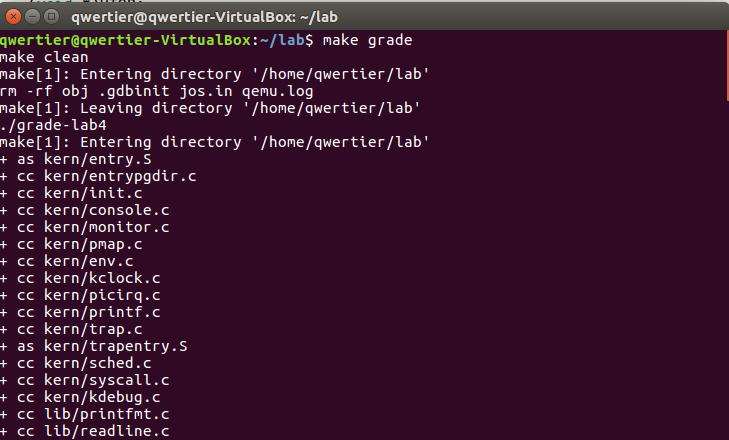
\includegraphics[width=6in]{figures/lab4/finish1.png}
  \caption{Lab4完成图}\label{fig:lab4:finish1}
\end{figure}

\begin{figure}[H]
  \centering
  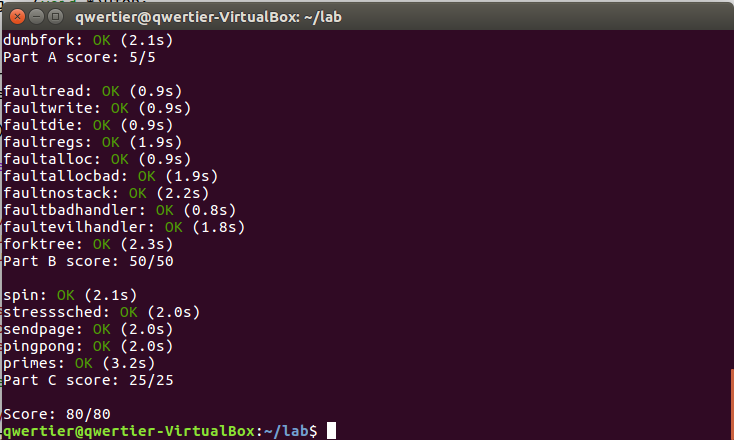
\includegraphics[width=6in]{figures/lab4/finish2.png}
  \caption{Lab4完成图}\label{fig:lab4:finish2}
\end{figure}


\end{ExerciseList}


\begin{ExerciseList}

  \setcounter{Exercise}{0}

  \section{Lab 5: File system, Spawn and Shell}

  \subsection{实验目的}

  在本实验中,我们将实现spawn一个加载和运行磁盘可执行文件的库调用。然后充实我们的内核和库操作系统,在控制台上运行一个shell。这些功能需要一个文件系统,本实验将介绍一个简单的读/写文件系统。

  \subsection{实验过程}

  \subsubsection{第一部分:文件系统实现}


  实验指导书首先简单介绍了一般文件系统的结构,包括扇区、块、超级块、块位图、文件元数据和目录的概念。在jos中不会实现一个真实的文件系统的全部功能。我们实现的操作系统不会包含权限的限制,默认是单用户操作系统。组织文件时不使用inode,而是直接使用元数据。为了存储更大的文件将使用一层间接块。

  \textbf{磁盘访问}

  当前jos操作系统中的文件系统环境需要能够访问磁盘,但我们还没有在内核中实现任何磁盘访问功能。除了采用传统的“单块”操作系统策略,即将IDE磁盘驱动程序与必要的系统调用一起添加到内核中以允许文件系统访问它之外,我们还将IDE磁盘驱动程序作为用户级文件的一部分系统环境。我们仍然需要稍微修改内核,以便进行设置,以便文件系统环境具有实现本身磁盘访问所需的权限。”


  \Exercise{首先要打开文件系统访问I/O的权限,在创建进程时判断如果是文件系统的进程,那么给与I/O访问权限。}

  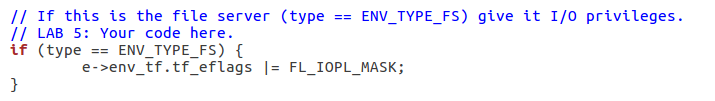
\includegraphics[width=6in]{figures/lab5/image64.png}

  
\includegraphics[width=6in]{figures/lab5/image65.png}

  问题1:

  回答:不用,切换进程时调用的pop\_tf函数中的iret指令恢复了包括eflags的寄存器。

  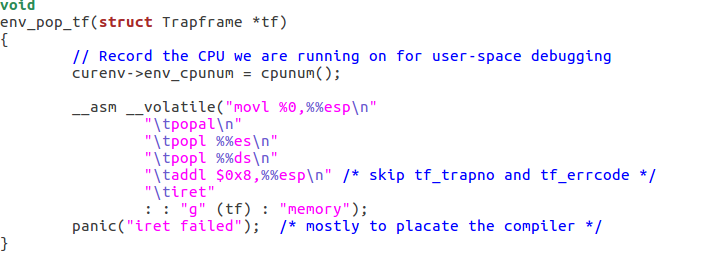
\includegraphics[width=6in]{figures/lab5/image67.png}

  \textbf{块缓存}

  Jos中我们通过缓存技术来实现访问磁盘块。该机制可以支持最大3GB的磁盘。

  我们将文件系统服务进程的虚拟地址空间(0x10000000 (DISKMAP)到0xD0000000 (DISKMAP+DISKMAX))对应到磁盘的地址空间(3GB)。

  由于现代磁盘大于3GB,在32位机器上的真正的文件系统实现会很麻烦。这种缓冲区高速缓存管理方法在64位地址空间的机器上仍然是合理的。

  映射方法:我们假装整个磁盘都已经被缓存到内存中,当我们想访问虚拟空间中的一个页时,由于虚拟空间还没有被映射,会发生页错误。在页错误处理程序中则会实际进行磁盘块到虚拟地址的映射并将该块磁盘内容缓存到内存中。

  此时就可以恢复文件系统进程进行正常的文件访问。

  \Exercise{Exercise2}

  Bc\_pgfault函数负责处理页面错误,处理的同时进行页面映射并从磁盘中缓存对应的块到内存中。

  处理的步骤:

  \begin{enumerate}
  \item 根据地址计算出对应的blockno(块编号)
  \item 检查地址范围是否超出(0x10000000 (DISKMAP)到0xD0000000 (DISKMAP+DISKMAX))的映射边界
  \item 检查块编号是否超出块数
  \item 将地址对齐到页起始位置
  \item 页面映射
  \item 调用ide\_read函数读取缓存块对应的数个磁盘页到内存中
  \item 更新脏位
  \end{enumerate}

  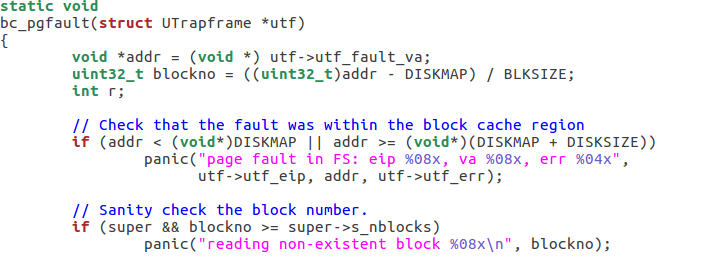
\includegraphics[width=6in]{figures/lab5/image69.png}

  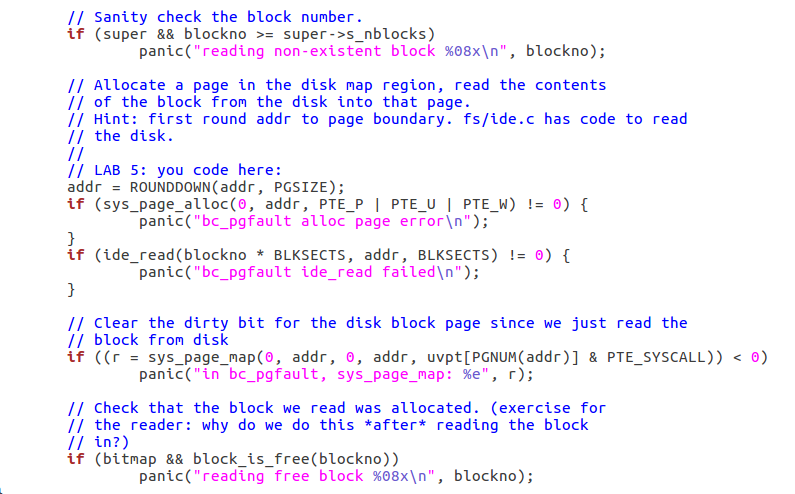
\includegraphics[width=6in]{figures/lab5/image70.png}

  Flush\_block函数负责将缓存中的块写回到磁盘中。

  处理步骤:

  \begin{enumerate}
  \item 根据地址计算出对应的blockno(块编号)
  \item 检查地址范围是否超出(0x10000000 (DISKMAP)到0xD0000000 (DISKMAP+DISKMAX))的映射边界
  \item 检查如果对应块没有映射就不写回
  \item 检查如果对应块不是脏块(没有发生改动)就不写回
  \item 最后将缓存写回到磁盘,检查是否成功并更新脏位
  \end{enumerate}

  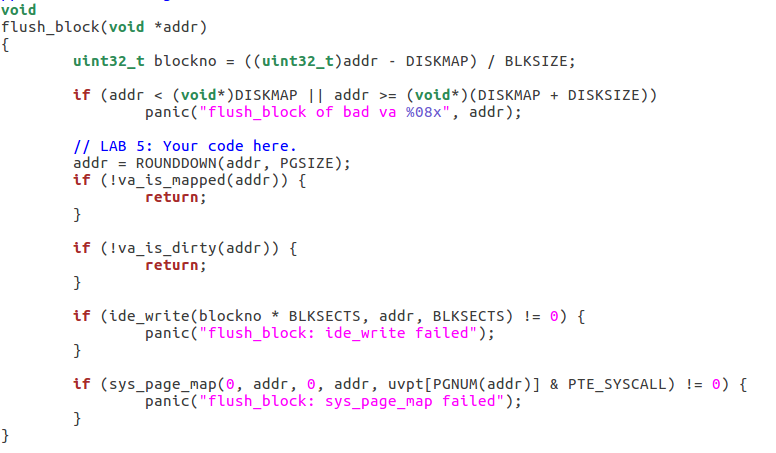
\includegraphics[width=6in]{figures/lab5/image71.png}

  通过make grade检查是否成功

  \includegraphics[width=6in]{figures/lab5/image72.png}

  \textbf{块分配表}

  Block bitmap记录磁盘上的一块是否写有内容。在fs\_init设置bitmap指针之后,我们可以将其bitmap视为一个打包的位数组,每个磁盘块对应一个位。我们可以使用block\_is\_free函数检查给定块在位图中是否被标记空的。

  \Exercise{Exercise3}

  依次遍历所有bitmap位,当发现bitmap的第i位为1(表示能用)时将此位赋0并返回块号i。

  \textbf{文件操作}

  在fs / fs.c中提供了各种函数来实现管理File的基本结构,扫描和管理目录文件的条目,从根目录文件系统来解析绝对路径名。

  \Exercise{此步需要实现实现 file\_block\_walk 和file\_get\_block函数。}

  Fs.c文件中编写了与文件操作有关的一系列操作,例如浏览目录,解析路径等。

  file\_block\_walk函数寻找一个文件结构f中的第fileno个块指向的磁盘块编号放入ppdiskbno。类似于遍历目录结构。

  \includegraphics[width=6in]{figures/lab5/image76.png}

  file\_get\_block函数先调用file\_walk\_block函数找到文件中的目标块,然后将其转换为地址空间中的地址赋值给blk。

  \includegraphics[width=6in]{figures/lab5/image77.png}

  \textbf{文件系统接口}

  \includegraphics[width=6in]{figures/lab5/image78.png}

  实现了文件系统内的函数后,我们需要向外界提供更方便的统一接口。

  虚线下面的所有内容都是从常规环境到文件系统环境的读取请求的机制。read(提供的接口)在任何文件描述符上工作,并简单地调度到适当的设备读取功能,在这种情况下 devfile\_read(我们可以有更多的设备类型,如管道)。 devfile\_read 实现read专门针对磁盘上的文件。这个和lib / file.c中的其他devfile\_*函数 实现了FS操作的客户端,并且都以大致相同的方式工作,将请求结构中的参数捆绑在一起,调用 发送IPC请求,解包并返回结果。该fsipc 函数只是处理向服务器发送请求和接收答复的常见细节。

  文件系统服务器代码可以在fs / serv.c中找到。它在serve函数中循环通过IPC接收请求,将该请求分派给相应的处理函数,并通过IPC发回结果。在读取的例子中, serve将调度到serve\_read,将处理特定的IPC细节读取请求,如解开请求结构,最后调用 file\_read实际执行文件读取。

  JOS的IPC机制让一个环境发送一个单一的32位数字,并可选择共享一个页面。为了将请求从客户端发送到服务器,我们使用32位数字作为请求类型(文件系统服务器的RPC编号,就像syscalls的编号一样)并将参数存储union Fsipc在页面上的请求中 通过IPC共享。在客户端,我们总是共享页面fsipcbuf; 在服务器端,我们在fsreq (0x0ffff000)处映射传入的请求页面。

  服务器也通过IPC发回响应。我们使用32位数字作为函数的返回码。对于大多数RPC,这是他们所有的返回值。 FSREQ\_READ并FSREQ\_STAT返回数据,他们只是写入客户端发送请求的页面。在响应IPC中不需要发送此页面,因为客户端首先将其与文件系统服务器共享。此外,在答复中,FSREQ\_OPEN与客户分享一个新的“Fd页”。我们很快会返回到文件描述符页面。

  观察服务端主循环轮询时处理文件操作的过程:

  \begin{enumerate}
  \item 从IPC接受1个请求类型req以及数据页fsreq
  \item 然后根据req来执行相应的服务端处理函数
  \item 将相应服务端函数的执行结果(如果产生了数据也则有pg)通过IPC发送回调用进程
  \item 将映射好的物理页fsreq取消映射
  \end{enumerate}

  \Exercise{Serve\_read函数用于读文件请求。从ipc结构体中获取需要读取的目标信息,调用file\_read函数读取文件放置在ret\_buf中。}

  \includegraphics[width=6in]{figures/lab5/image80.png}

  \Exercise{serve\_write同样是获取请求信息,将req\_buf中的文件内容写入到磁盘块。}

  \includegraphics[width=6in]{figures/lab5/image83.png}

  Devfile\_write函数主要功能是将写文件需求通过fsipc打包成请求以便于发送给文件服务系统。

  \includegraphics[width=6in]{figures/lab5/image84.png}

  \subsubsection{第二部分:Spawning过程}

  \textbf{环境继承}

  Spawn函数可以从父进程中调用,装载一个新的程序执行,类似于UNIX的fork后直接exec装载新的程序。
  Exercise7

  sys\_env\_set\_trapframe将父进程的环境(寄存器)复制为子进程的环境。

  \includegraphics[width=6in]{figures/lab5/image86.png}

  加入系统调用

  \includegraphics[width=6in]{figures/lab5/image87.png}

  使用make run-spawnhello可以看到父进程的信息和子进程的信息都输出了,输出中间的fs文件系统检查内容是由于多进程交替执行输出到控制台的结果。

  \includegraphics[width=6in]{figures/lab5/image88.png}

  \textbf{在fork和spawn之间共享库状态}

  UNIX文件描述符包括pipe,console I/O。 在JOS中,这些设备类型都有1个与与它关联的struct Dev,里面有实现read/write等文件操作的函数指针。在lib/fd.c中实现了传统UNIX的文件描述符接口。

    在lib/fd.c中也包括每个客户进程的文件描述符表布局,开始于FSTABLE。这块空间为每个描述符保留了1个页的地址空间。 在任何时候,只有当文件描述符在使用中才在文件描述符表中映射页。

    我们想要共享文件描述符状态在调用fork和spawn创建新进程。当下,fork函数使用COW会将状态复制1份而不是共享。在spawn中,状态则不会被拷贝而是完全舍弃。

    所以我们将改变fork来共享状态。在inc/lib.h中新定义了PTE\_SHARE位来标识页共享。当页表入口中设置了该位,则在fork和spawn时应该从父进程中拷贝PTE映射到子进程。

  \Exercise{在duppage中添加对PTE\_SHARE位进行判断,若有PTE\_SHARE位则直接复制映射。}

  \includegraphics[width=6in]{figures/lab5/image90.png}

  在copy\_shared\_pages中扫描进程中所有页,发现PTE\_SHARE标记时,调用sys\_page\_map进行映射复制。

  \includegraphics[width=6in]{figures/lab5/image91.png}

  运行make run-testpteshare,可以看到"fork handles PTE\_SHARE right" 和 "spawn handles PTE\_SHARE right"

  运行make run-testfdsharing,可以看到"read in child succeeded" 和 "read in parent succeeded"

  \subsubsection{第三部分:Shell}

  \textbf{键盘接口}

  为了使shell工作,我们需要一种方法来输入它。QEMU一直在显示我们写到CGA显示器和串行端口的输出,但到目前为止,我们只在内核监视器上进行输入。在QEMU中,输入在图形窗口中的输入显示为从键盘到JOS的输入,而输入到控制台的输入在串行端口上显示为字符。 kern / console.c已经包含了自实验1以来已被内核监视器使用的键盘和串口驱动程序,但是现在我们需要将这些驱动程序附加到系统的其他部分。

  \Exercise{在trap.c中添加对于IRQ\_OFFSET+IRQ\_KBD和IRQ\_OFFSET+IRQ\_SERIAL的判断,分别调用kbd\_intr和serial\_intr进行处理。}

  \includegraphics[width=6in]{figures/lab5/image96.png}

  运行make run-testkbd测试:

  \includegraphics[width=6in]{figures/lab5/image97.png}

  \textbf{Shell命令}

  首先运行make run-icode测试

  echo hello world | cat 将hello world文本传送给cat程序,cat程序用来显示文本

  \includegraphics[width=6in]{figures/lab5/image98.png}

  cat lorem |cat 显示文本再传送给cat

  \includegraphics[width=6in]{figures/lab5/image99.png}

  cat lorem |num 给文本加上行号

  \includegraphics[width=6in]{figures/lab5/image100.png}

  cat lorem |num |num |num |num |num将加上行号的文本作为新文本再添加行号,多次迭代

  \includegraphics[width=6in]{figures/lab5/image101.png}

  lsfd

  \includegraphics[width=6in]{figures/lab5/image102.png}

  \Exercise{要求我们实现shell的重定向特性,使用open()打开文件来获得命令输入。}

  运行make run-testshell来测试shell功能,成功重定向。

\end{ExerciseList}


\chapter{xv6实验系统分析}

\section{xv6的系统结构}

SMP是Symmetric Multi Processing的简称,意为对称多处理计算机系统,内有许多紧耦合多处理器,这种系统的最大特点就是共享所有资源。在SMP架构中,每个处理器在功 能上都是对称、等价的。每个处理器有独自的中断处理控制器(硬件)。 内存在所有处理器之间共享。因此处理器可以通过共享的内存区域进行通讯。Xv6就是一个SMP操作系统,可以有多个cpu公共工作.

xv6基于典型的UNIX操作系统设计思路。简单地说,xv6是一种能区分内核态和用户态,基于扁平内存管理的层次型单体内核,应用程序和操作系统是处于不同的特权状态和地址空间。代表应用程序的用户态进程运行在CPU的用户态(又称非特权模式,用户模式),无法直接访问系统硬件和操作系统中的系统数据,而操作系统运行在CPU的核心态(又称特权模式,内核模式),可以访问系统硬件和核心数据。下面给出一个xv6系统结构是示意图

\includegraphics[width=6in]{figures/struct/fig1.png}

下面分别从系统调用接口、进程/线程管理、内存管理、文件系统、I/O管理等几个方面进行总体分析。

进程通过系统调用使用内核服务。系统调用是应用程序访问操作系统的接口。在系统调用接口上,通用操作系统与基于此操作系统的应用程序处于两个不同的CPU特权态,操作系统处于核心态,而应用程序处于用户态。在核心态可以执行CPU特权指令,而用户态无法执行特权指令,且只能通过特定的指令或中断来访问操作系统提供的各种功能。这在一定程度上保证了系统整体的安全,避免应用程序对操作系统可能的破坏。内核使用了 CPU 的硬件保护机制来保证用户进程只能访问自己的内存空间。内核拥有实现保护机制所需的硬件权限(hardware privileges),而用户程序没有这些权限。当一个用户程序进行一次系统调用时,硬件会提升特权级并且开始执行一些内核中预定义的功能。内核提供的一系列系统调用就是用户程序可见的操作系统接口,xv6 内核提供了 Unix 传统系统调用的一部分,它们是:

\includegraphics[width=6in]{figures/struct/fig2.png}

\includegraphics[width=6in]{figures/struct/fig3.png}

在内存管理方面,通用操作系统采用了虚拟内存管理方式,这样可以让内存需求超过实际物理内存的进程/线程能够执行,其主要思想是把重要和常用的数据和执行代码放在物理内存中,把不常用的数据和执行代码放到二级存储(这里主要指的是硬盘等可在掉电后保存数据的存储介质),随时根据系统执行情况替换放在内存中的数据和代码。而且通过虚存管理可以实现对不同内存区域的保护,不同进程之间,或者应用程序和操作系统之间的地址空间相对隔离。这样一般情况下不同进程的地址空间不能直接访问,且应用程序不能直接访问内核地址空间。所以一个与错误的应用程序不会导致系统的崩溃,从而增加了系统的可靠性。xv6操作系统没有采用虚拟内存管理,而是采用了简单的基于X86段模式的单一地址空间管理方式。在内存分配和释放的管理上,xv6相对实现得比较简单,采用基于可变分区分配的首次适配算法,容易产生内存碎片。

在进程/线程管理方面,当前通用操作系统结合虚存管理,采用进程和线程结合的管理方式。进程代表了一个程序执行的过程以及其所占用的计算机资源(包括CPU、内存、文件等),进程的执行流可用线程来表示。操作系统的调度单位可以是进程或线程。一个进程可以包含多个线程,属于同一进程的多个线程共享进程管理的资源,比如属于同一进程的多个线程共享进程所管理的内存,这样这些线程可以直接访问属于进程的全局地址空间。 xv6操作系统实现了一个基于进程(没有实现线程)的简单进程管理机制。

在文件系统管理方面,当前通用操作系统结合虚存管理,实现了多种复杂、高效且可靠的文件系统,且建立了一个统一的虚拟文件系统层,屏蔽不同文件系统的差异,对上层提供统一的接口。且与用户管理和进程管理结合,可实现安全管理,保证对文件的安全访问。xv6操作系统实现了一个相对简单的基于inode索引方式的文件系统。

在I/O管理方面,xv6操作系统与通用操作系统(特别是类UNIX操作系统)差别不是特别大,都把设备“看成”是一种特殊的设备文件,有设备号,用文件的访问接口来进行打开、关闭、读、写和控制等操作。在灵活性方面,xv6驱动程序不能象通用操作系统那样根据硬件情况动态加载,而是在编译时候就静态确定的。


\section{引导}

\begin{itemize}
\item bootloader是什么?
\item bootloader做了哪些事情?
\item xv6是如何被加载并启动的?
\item xv6如何实现内核态到用户态的转变的?
\item xv6启动用户态进程前需要完成哪些事情?
\end{itemize}

\subsection{开始}

当计算机加电后,一般不直接执行操作系统,而是执行引导加载程序。简单地说,引导加载程序就是在操作系统内核运行之前运行的一段小程序。通过这段小程序,我们可以初始化硬件设备、建立系统的内存空间映射图,从而将系统的软硬件环境带到一个合适的状态,以便为最终调用操作系统内核准备好正确的环境。最终引导加载程序把操作系统内核映像加载到RAM中,并将系统控制权传递给它。下面是一个通用操作系统的启动过程。

\includegraphics[width=6in]{figures/boot/fig1.png}


引导加载程序(bootloader)是系统加电后运行的第一段软件代码。对于PC386的体系结构而言,PC机中的引导加载程序由BIOS (Basic Input Output System,即基本输入/输出系统,其本质是一个固化在主板Flash/CMOS上的软件)和位于软盘/硬盘引导扇区中的OS Boot Loader一起组成。BIOS实际上是被固化在计算机ROM(只读存储器)芯片上的一个特殊的软件,为上层软件提供最底层的、最直接的硬件控制与支持。更形象地说,BIOS就是PC计算机硬件与上层软件程序之间的一个"桥梁",负责访问和控制硬件。

以PC386为例,计算机加电后,CPU从物理地址0x000FFFF0(由初始化的CS:EIP确定,此时CS和IP的值分别是0xF000和0xFFF0))开始执行。在0x000FFFF0这里只是存放了一条跳转指令,通过跳转指令跳到BIOS例行程序起始点。BIOS做完计算机硬件自检和初始化后,会选择一个启动设备(例如软盘、硬盘、光盘等),并且读取该设备的第一扇区(即启动扇区)到内存一个特定的地址0x7c00处,然后CPU控制权会转移到那个地址继续执行。至此BIOS的初始化工作做完了,进一步的工作交给了xv6。

\subsection{xv6启动}

整个xv6系统的启动流程大致是这样的:首先BIOS将把OS的Boot Loader从磁盘上(一般是位于第一个扇区)拷贝到内存当中。当BIOS将基本的初始化程序完成后,将跳转到Boot Loader所在内存的位置继续执行。 Boot Loader将把OS的内核从磁盘上拷贝到然后运行。这样就完成了启动。

在xv6的源码中,整个启动过程主要牵涉到bootasm.S和bootmain.c两个文件

\subsubsection{bootloader代码分析}

\textbf{bootloader的组成}


bootloader包含两个文件,bootasm.S和bootmain.c。生成的bootloader会写到一个主引导扇区上面。作为主引导扇区,其位置在软盘或硬盘的第一个扇区,其大小为512个字节,在此扇区的最后两个字节是一个主引导扇区特征码为”55AA”。Makefile的97行和98行是通过gcc把 bootmain.c和bootasm.S编译成目标文件bootmain.o和bootasm.o。Makefile的99行是通过ld程序把目标文件bootmain.o和bootasm.o链接成目标文件bootblock.o,且定义了起始执行的点(也称入口点)为start函数,具体的代码段起始地址为0x7C00。Makefile的100行是通过objdump程序把bootblock.o反汇编成bootlock.asm。Makefile的101行是通过objcopy程序把bootblock.o变成二进制码bootlock。Makefile的102行是通过sign.pl程序把bootlock扩展到512个字节,并把最后两个字节写成”55AA”。

bootloader的启动主要涉及到bootasm.S、bootmain.c。其中bootasm.S的主要作用是从实模式转化到保护模式。 bootmain的作用是把内核从磁盘拷贝到内存中。

\subsubsection{bootasm.S}

在进入实模式向保护模式切换之前,首先需要把中断关闭("cli" at line 13),保证转换过程不被硬件中断打断。

\includegraphics[width=6in]{figures/boot/fig3.png}


但是实模式刚运行完,很多遗留下的一些寄存器的值需要我们整理下,所以我们需要“在16~19行中 将\%ax 置零,然后把这个零值拷贝到三个段寄存器中, 将DS, ES, SS进行清零”。

实模式的东西处理完,我们的重点是要转换到保护模式中去开始真正的工作。为此我们需要打开A20开关, 将32位地址总线打开,使得地址位从20位切换到32位.

关于为什么需要打开A20开关,可以参考文档最后的附录部分.

下面的代码实现了打开A20开关.

\includegraphics[width=6in]{figures/boot/fig4.png}

接下来加载全局符号表GDT

第42行代码通过引导加载器执行 lgdt指令来把指向 gdt 的指针 gdtdesc加载到全局描述符表(GDT)寄存器中。第44行正式开启保护模式(CR0\_PE=1)接下来第51行处理器还需要将16位模式(因为之前是实模式,所以目前还是处于16位的模式)切换到32位。由于我们没法直接修改 \%cs,所以使用了一个 ljmp 指令ljmp \$(SEG\_KCODE<<3), \$start32。跳转指令会接着在下一行执行,但这样做实际上将 \%cs 指向了 gdt 中的一个代码描述符表项。该描述符描述了一个32位代码段,这样处理器就切换到了32位模式下。

\includegraphics[width=6in]{figures/boot/fig5.png}

接下来完成保护模式之下的初始化数据,然后开始执行bootmain.c代码

\includegraphics[width=6in]{figures/boot/fig6.png}

\subsubsection{bootmain.c}

在这个文件中主要有四个函数:bootmain、waitdisk、readsect和readseg。其中bootmain是加载内核,其余三个都是对磁盘进行访问的程序。

首先来看一下waitdisk、readsect和readseg。 readseg函数的作用是从磁盘的offset处开始读取count个字符到pa处。在读取数据时是通过调用readsect以扇区为单位进行的。因此在86行保证pa是从一个扇区起始位置开始,因此要对pa进行对齐。readsect是对磁盘进行读取,在读取之前每次调用waitdisk等待磁盘的准备过程,一旦磁盘准备好后就可以进行读取了。

\includegraphics[width=6in]{figures/boot/fig7.png}

\includegraphics[width=6in]{figures/boot/fig8.png}

\includegraphics[width=6in]{figures/boot/fig9.png}

然后看一下bootmain过程。bootmain的目的是从磁盘中加载内核到内存中,其中内核是 ELF 格式的二进制文件。为了读取 ELF 头,在第28行bootmain 载入 ELF 文件的前4096字节,并将其拷贝到内存中 0x10000 处。其中包含了ELF执行文件格式的头。从中可以知道读取镜像的大小以及存放的位置

第31行通过 ELF 头检查这是否的确是一个 ELF 文件。

在第39行bootmain 调用 readseg 将数据从磁盘中载入,第41行并调用 stosb 将段的剩余部分置零。stosb使用 x86 指令 rep stosb 来初始化内存块中的每个字节。当完成拷贝后,在第46行bootmain获取内核入口程序的地址,然后进入该入口

bootloader紧接着就是entry开始运行,这个时候x86 的分页硬件在此时还没有开始工作;所以这时的虚拟地址是直接映射到物理地址上的。

boot loader 把 xv6 内核装载到物理地址 0x100000 处。之所以没有装载到内核指令和内核数据应该出现的 0x80100000,是因为小型机器上很可能没有这么大的物理内存。而之所以在 0x100000 而不是 0x0 则是因为地址 0xa0000 到 0x100000 是属于 I/O 设备的。

为了让内核的剩余部分能够运行,entry 的代码设置了页表,将 0x80000000开始的虚拟地址映射到物理地址 0x0 处。

\includegraphics[width=6in]{figures/boot/fig10.png}

Entry 在完成设置页表和栈指针的操作之后,跳转到内核的 C 代码,并在内存的高地址中执行它了。
首先它将栈指针 %esp 指向被用作栈的一段内存。所有的符号包括 stack 都在高地址,所以当低地址的映射被移除时,栈仍然是可用的。
entry 跳转到高地址的 main 代码中。我们必须使用间接跳转,否则汇编器会生成 PC 相关的直接跳转(PC-relative direct jump),而该跳转会运行在内存低地址处的 main。 main 不会返回,因为栈上并没有返回 PC 值。好了,现在内核已经运行在高地址处的函数 main中了。

到现在为止,xv6的引导工作全部完成,接下来开始执行内核代码.


\section{进程与调度分析}

\subsection{进程的概念}

程序与进程的概念是不可分的。当用户在计算机上运行一个程序时,此程序对应的进程就诞生了,并实际完成各种程序提供的功能,而用户关闭一个程序时,进程也随之终止。程序是为了完成某项任务编排的语句序列,它要告诉计算机如何执行,因此程序是需要通过CPU来运行的,且在程序的运行过程中需要占有计算机的各种资源(比如内存等)才能运行下去。

如果计算机系统在任一时刻限制只有一个程序在运行,则程序在整个运行过程中独占计算机中的全部资源,这样整个程序运行和管理就简单了。就象在一个家中只住了一个人A,他想看书就到书房去看书,想睡觉就到睡房的床上去睡觉,想看电视就到电视厅看电视,想吃饭就去餐厅吃饭,没人和他抢占资源。但为了提高计算机系统的资源利用率,需要支持多个程序并发执行。这就会带来许多新的问题,如资源的共享与竞争,同步与互斥等。

比如此人与B成家并有了小孩C,那就是三口之家同时住一套房,当A想去看足球比赛直播电视节目的时候,如果发现电视厅已经有B在坐着看连续剧电视节目了,A就得等待或干别的事情。除非A在买一个电视,并在另外一个房间看他的球比赛直播。

由于程序是静态的,我们看到的程序是存储在存储介质(如硬盘、光盘等)上的,它无法反映出程序执行过程中的动态特性,而且程序在执行过程中会不断申请资源或释放资源,这样让程序作为共享资源的基本单位是不合适的,所以需要引入一个概念,它能描述程序的执行过程而且可以作为共享资源的基本单位,这个概念就是进程。简单地说,一个进程是一个具有一定独立功能的程序在一个数据集合上的一次动态执行过程。每个进程都是整个应用的某一部分。操作系统在逻辑上维护了进程的运行状态信息,即与进程运行直接相关的CPU寄存器和栈空间(只有这样才能实现进程切换)。操作系统根据当前进程的情况设置进程的状态,并根据进程的状态(比如优先级)进行选择一个进程占用CPU并运行,这个过程成为调度。

\subsection{进程控制块}

程序的运行是通过进程体现的,操作系统对进程进行管理和控制,那么操作系统怎么了解到进程的状态并掌握进程占有的资源分配呢,而且进程做状态转换时CPU的现场保存在那呢?这实际是通过进程控制快(Process Control Block, 简称PCB)。PCB是进程 的唯一标志,在其中记录了进程的全部信息,相当于进程的档案。操作系统通过PCB感知进程的存在,通过PCB了解进程和控制 进程的运行。在xv6中,所有的CPU共享一个进程控制块池,即源代码中为proc.c中的proc(即进程控制块)数组。在这 个进程数组保存的进程控制块结构分成两类:一类是未使用的进程控制块结构,另一类是正在使用的进程控制块结构。每次要创建一个进程时,只需要从进程控制块数组中取得一个未使用进程控制块结构进行相应的处理即可。

xv6中结构体 struct proc包含进程大小、页表、内核栈、进程状态、进程id、父进程、目录等等,代码如下:

\includegraphics[width=6in]{figures/process/fig2.png}

\begin{itemize}
\item sz是记录进程所占有的内存空间大小;
\item pgdir记录了进程页表的线性地址
\item kstack是进程在内核态的栈;
\item 枚举类型变量 state记录了进程的状态;
\item pid是进程的ID;
\item parent记录父进程;
\item tf是当前系统调用的中断帧;
\item context是切换进程需要维护的硬件寄存器内容, 是进程运行的入口;
\item chan不为NULL时,是进程睡眠时所挂的睡眠队列;
\item killed不为0时,表示进程被杀死了;
\item ofile数组是进程打开的文件数组;
\item cwd是进程运行时所处的当前目录;
\item name保存了进程的名字(用于调试)。
\end{itemize}

struct proc在proc.h中,并且在该文件之中定义了几个关键的数据结构。其中context是在内核进行上下文切换需要保存的寄存器: edi,esi,ebx,ebp,eip.

\includegraphics[width=6in]{figures/process/fig3.png}

proc[NPROC]数组(在proc.c文件的12行)定义了xv6所能够支持的进程所需的相关数据,NPROC表示了xv6可支持进程个数。

\includegraphics[width=6in]{figures/process/fig4.png}

cpu结构是记录计算机中所有CPU的相关信息:

\includegraphics[width=6in]{figures/process/fig5.png}

其中:

\begin{itemize}
\item apicid 代表此CPU的id编号;
\item scheduler表示scheduler的地址
\item ts是Task state segment,用于在中断时找到栈
\item gdt是此CPU的全局描述符表(GDT);
\item started表示是否此CPU已经启动了;
\item ncli表示执行pushcli函数的次数;
\item intena表示是否能被打断;
\item curproc是当前正在此CPU上运行的进程控制块;
\end{itemize}

spinlock的作用在于当进程请求得到一个正在被占用的锁时,将进程处于循环检查,等待锁被释放的状态。

\includegraphics[width=6in]{figures/process/fig6.png}

进程在虚拟内存中的布局如下:

\includegraphics[width=6in]{figures/process/fig7.png}

Xv6使用了一些全局变量来记录进程的状态.
进程数组 proc[NPROC]数组就是进程池。
进程池访问锁 proc\_table\_lock是一个spinlock是用来保护对进程池的临界区访问。
当前运行进程 curproc则是记录每个cpu当前运行的进程。
第一个进程 initproc是记录第一个创立的进程。这个进程十分特殊,它将托管所有没有父进程的进程(也就是父进程先于子进程结束)。
下一进程号 nextid是用来产生进程号的,在系统启动后会一直保持递增。

\subsection{进程的状态}

进程从诞生到死亡要经历若干个阶段,也会有生老病死。简单地说,进程有三种状态:就绪、执行、等待。多种原因可以导致创建一个进程,比如,当操作系统把一个程序从硬盘调入内存后,在开始执行前,操作系统就要为此程序创建一个对应的进程。又比如,一个进程可以自己创建一个子进程,子进程被创建后就是在内存中,处于就绪态,所谓就绪态就是万事具备,只欠CPU这个东风了;一旦进程占有了CPU,就可以执行实际的工作了,其状态就变成了执行态;进程在执行中如果需要等待某个资源(如等硬盘输入数据),则进程会放弃CPU,且其状态就变为等待态,这时操作系统又会从处于就绪态的另一个进程中挑选一个进程占有CPU,则这另一个进程的状态就变成了执行态。当前一个进程所等到数据到来后,处于等待态的前一个进程又被唤醒,并把状态变成为就绪态。

在实际的操作系统中,进程的状态往往多于三种,比如找xv6中,进程具有多种状态,包括:EMBRO, SLEEPING, RUNNABLE, RUNNING和ZOMBIE。定义在proc.h文件中:

\mint{C}{enum proc_state { UNUSED, EMBRYO, SLEEPING, RUNNABLE, RUNNING, ZOMBIE };}

状态的含义如下:

\begin{itemize}
\item UNUSED:进程未被创建(即进程控制块空闲)时的状态;
\item EMBRYO:需要分配一个进程控制块且找到一个处于UNUSED状态的进程控制块时,把此进程控制块状态设置为要使用的状态;
\item SLEEPING:进程由于等待某资源等原因无法执行,进入睡眠状态,即等待态;
\item RUNNABLE:进程获得了除CPU之外的所有资源,处于可运行状态,即就绪态;
\item RUNNING:进程获得CPU,正在运行的状态,即执行态;
\item ZOMBIE:进程结束的状态
\end{itemize}

\subsection{Xv6对于进程的处理过程}

与进程相关的处理函数集中在proc.c中,下面将依次介绍相关处理过程。

\subsubsection{进程管理初始化}

pinit过程仅仅是初始化proc\_table\_lock锁。

\subsubsection{初始化用户进程init}

userinit是初始化第一个用户进程init。其处理过程如下所示:

userinit首先调用allocproc。allocproc(第126行)的工作是在页表中分配一个槽(即结构体 struct proc),并初始化进程的状态,为其内核线程的运行做准备。

allocproc会在proc的表中找到一个标记为 UNUSED的槽位。当它找到这样一个未被使用的槽位后,allocproc 将其状态设置为 EMBRYO,使其被标记为被使用的并给这个进程一个独有的 pid。接下来,它尝试为进程的内核线程分配内核栈。如果分配失败了,allocproc 会把这个槽位的状态恢复为 UNUSED 并返回0以标记失败。

\includegraphics[width=6in]{figures/process/fig8.png}

\subsubsection{创建子进程}

在xv6中,可以通fork来复制父进程内容并创建一个新的子进程。其处理过程如下所示:

一个进程调用 fork() 函数后,系统先给新的进程分配资源,例如存储数据和代码的空间。然后把原来的进程的所有值都复制到新的新进程中,只有少数值与原来的进程的值不同。相当于克隆了一个自己。fork() 函数通过系统调用创建一个与原来进程几乎完全相同的进程,也就是两个进程可以做完全相同的事(即复制了 fork() 函数后的代码),但如果初始参数或者传入的变量不同,两个进程也可以做不同的事。需要注意的是,两个进程拥有不同的内存空间和寄存器(fork()函数之前的变量值是一样的,但存储在不同地方),改变一个进程中的变量不会影响另一个进程。

fork()调用的一个奇妙之处就是它仅仅被调用一次,却能够返回两次,它可能有三种不同的返回值:

\begin{itemize}
\item 在父进程中,fork() 返回新创建子进程的进程pid;
\item 在子进程中,fork() 返回0;
\item 如果出现错误,fork() 返回一个负值;
\end{itemize}

不同的进程有一个唯一的不同进程pid,通过 getpid() 函数可以知道当前进程pid,可以说我们就是通过这个pid知道当前所在进程。

创建新进程成功后,系统中出现两个基本完全相同的进程,这两个进程执行没有固定的先后顺序,哪个进程先执行要看系统的进程调度策略。

\subsubsection{调度进程}

任何操作系统都可能碰到进程数多于处理器数的情况,这样就需要考虑如何分享处理器资源。理想的做法是让分享机制对进程透明。通常我们对进程造成一个自己独占处理器的假象,然后让操作系统的 多路复用机制(multiplex) 将单独的一个物理处理器模拟为多个虚拟处理器。

记下来介绍 xv6 是如何调度进程.
Xv6系统允许有多个cpu,并且每一个cpu获取进程调度的权利是相同的。CPU在scheduler里面进行轮询操作,每次从线程池中选择一个RUNNABLE的进程进行运行。直到运行完毕,或一单位时间片结束,或者进程主动yield或sleep。
进程调度的时机:处于运行状态下的进程如果发生等待事件或者时间耗尽就会被xv6强制终止,变成就绪状态.这样的话,cpu就可以执行其他的进程,提高了cpu的使用率.

Xv6要完成进程切换的功能需要实现从运行中的一个进程切换到另一个进程并且让上下文切换透明化,还有就是xv6支持多个cpu,所以可能出现多个 CPU 同时切换进程的情况,那么我们必须使用一个带锁的方案来避免竞争,最后还有进程退出时必须释放其占用内存与资源.

进程切换:当CPU启动之后,执行scheduler函数,无限循环。在每个周期里,从进程表中找到一个RUNNABLE的进程,切换为进程的上下文,此时开始执行函数。当函数运行结束时,调用return函数,此时切换为CPU的上下文,开始下一循环。

进程唤醒与睡眠:如果一个程序需要等待IO,则CPU会将其设置为睡眠状态,此时不能被执行。当IO信号到达时,执行的进程会将IO信号对应的进程设置为RUNNABLE,即唤醒。下一个scheduler周期的时候,该进程就可能会被执行,处理IO信号。

进程表锁:对于多处理器架构而言,需要用到进程表的时候都需要事先获得表的锁,当结束之后再释放,这样保证了对进程表操作的原子化,可以避免多处理器的竞争问题。

下面通过代码来具体介绍xv6如何实现进程调度部分.
scheduler对每个CPU进行进程调度。CPU到没有运行用户进程时,就会进入这个过程中。这个过程不停的从进程中选出一个RUNNABLE的进程,然后运行这个进程(通过swtch.S中的swtch函数进行)。

\includegraphics[width=6in]{figures/process/fig9.png}

sched是放弃当前的用户进程,进入scheduler()。只需用通过swtch进行上下文切换即可。

\includegraphics[width=6in]{figures/process/fig10.png}

\subsubsection{设置用户进程返回}

forkret是用于新fork的进程进行返回地址用的。由于调用sys\_fork创建的新进程是通过shceduler()调用的,因此运行之前需要把proc\_table\_lock锁释放。

\includegraphics[width=6in]{figures/process/fig11.png}

sleep功能是让进程休眠。首先获得proc\_table\_lock,然后将记录chan,也就是说只有相关的chan才能把其唤起。然后调用sched()。当期被唤醒是,将继续运行,此时将chan等记录清空,并且将proc\_table\_lock锁释放,而获得lk锁。

\subsubsection{睡眠进程}

sleep功能是让进程休眠。首先获得proc\_table\_lock,然后将记录chan,也就是说只有相关的chan才能把其唤起。然后调用sched()。当期被唤醒是,将继续运行,此时将chan等记录清空,并且将proc\_table\_lock锁释放,而获得lk锁。

\includegraphics[width=6in]{figures/process/fig12.png}

\subsubsection{唤醒进程}

值得注意的是,使进程进入睡眠需要两个锁,lk和ptable.lock,由于之前已经得到了ptable.lock,所以wakeup在此期间不会执行,直至进程完全进入睡眠状态,所以lk这个锁可以释放。
wakeup函数的主体部分位于wakeup1函数中。

wakeup功能是唤醒进程。先获取proc\_table\_lock,然后调用函数wakeup1,然后释放proc\_table\_lock。

wakeup1是将由于chan休眠的进程都唤醒,即把进程的状态由SLEEPING改成RUNNABLE。

\includegraphics[width=6in]{figures/process/fig13.png}

\subsubsection{杀死进程}

kill的作用是杀死某个进程。只需要从进程池中找到拥有相应进程ID的进程,将其killed状态置1即可。如果目标进程出于sleeping状态则将其设置成RUNNABLE使其尽早被杀掉。

详细的代码如下所示.

\includegraphics[width=6in]{figures/process/fig14.png}

\subsubsection{退出进程}

exit完成了进程结束时的资源释放以及子进程处理等工作。在退出之前,用户进程需要关闭打开的文件(238-243行),将打开的文件夹关闭(358~359)。同时唤醒父进程,因为其可能出于wait状态。并将其子进程托管于init。然后改变其状态为ZOMBIE(等待父进程进行回收)。最后调用sched放弃CPU。

  \subsubsection{等待进程结束}

  wait是用于父进程等待子进程结束只用的。做法是不断的循环知道找到一个子进程变成ZOMBIE状态,则释放ZOMBIE子进程(回收其资源),然后结束循环返回其子进程的进程ID。在循环的时候需要判断是否被外部进程Kill,或有无活跃子进程,如果被杀死或无活跃子进程,则推出循环。

  \includegraphics[width=6in]{figures/process/fig16.png}


\section{内存管理}

内存管理机制是实时操作系统的重要组成部分。操作系统通过页表机制实现了对内存空间的控制。页表使得 xv6 能够让不同进程各自的地址空间映射到相同的物理内存上,还能够为不同进程的内存提供保护。除此之外,我们还能够通过使用页表来间接地实现一些特殊功能。xv6 主要利用页表来区分多个地址空间,保护内存。另外,它也使用了一些简单的技巧, 即把不同地址空间的多段内存映射到同一段物理内存(内核部分),在同一地址空间中多次映射同一段物理内存(用户部分的每一页都会映射到内核部分),以及通过一个没有映射的页保护用户栈。下面我们就来详细介绍一下 xv6 的内存管理.

xv6 初始化之后的物理内存图:

\includegraphics[width=6in]{figures/mem/fig1.png}

下面这个图展示的是 XV6 中虚拟地址到物理地址的映射关系.

\includegraphics[width=6in]{figures/mem/fig2.png}

xv6 使用页表(由硬件实现)来为每个进程提供其独有的地址空间。页表将虚拟地址(x86 指令所使用的地址)翻译(或说“映射”)为物理地址(处理器芯片向主存发送的地址).  Xv6实现了两级页表, 第一级页表有 1024 项 (占有 4096 字节), 第二级页表也有 1024 项 (占有4096 字节), xv6 为每一个进程分配了这样的一个二级页表来实现将进程的虚拟地址转化为物理地址的过程. 分页硬件使用虚拟地址的高 10 位来决定对应页目录条目。如果想要的条目已经放在了页目录中,分页硬件就会继续使用接下来的 10 位来从页表页中选择出对应的 PTE。否则,分页硬件就会抛出错误。通常情况下,大部分虚拟地址不会进行映射,而这样的二级结构就使得页目录可以忽略那些没有任何映射的页表页。在分页机制之中, 虚拟地址的高 20 位来找到该虚拟地址在页表中的索引,然后把其高 20 位替换为对应 PTE 的 PPN。而低 12 位

是会被分页硬件原样复制的。因此在虚拟地址-物理地址的翻译机制下,页表可以为操作系统     提供对一块块大小为 4096(2ˆ12)字节的内存片,这样的一个内存片就是一页。

\includegraphics[width=6in]{figures/mem/fig3.png}

从图中可以看到, 每个 PTE 都包含一些标志位,说明分页硬件对应的虚拟地址的使用权限。PTE\_P 表示 PTE 是否陈列在页表中:如果不是,那么一个对该页的引用会引发错误(也就是:不允许被使用)。PTE\_W 控制着能否对页执行写操作;如果不能,则只允许对其进行读操作和取指令。PTE\_U 控制着用户程序能否使用该页;如果不能,则只有内核能够使用该页。图 2-1 对此进行了说明。这些的标志位和页表硬件相关的结构体都在 mmu.h 定义。

\includegraphics[width=6in]{figures/mem/fig4.png}

每个进程都有自己的页表,xv6 会在进程切换时通知分页硬件切换页表。如图所示,

\includegraphics[width=6in]{figures/mem/fig5.png}

进程的用户内存从 0 开始,最多能够增长到 KERNBASE , 这使得一个进程最多只能使用 2GB 的内存。当进程向 xv6 要求更多的内存时,xv6 首先要找到空闲的物理页,然后把这些页对应的  PTE  加入该进程的页表中,并让  PTE  指向对应的物理页。xv6  设置了PTE 中的 PTE\_U、PTE\_W 、PTE\_P 标志位。大多数进程是用不完整个内存空间的;xv6 会把没有被使用的 PTE 的 PTE\_P 标志位设为 0。不同进程的页表将其用户内存映射到不同的物理内存中,因此每个进程就拥有了私有的用户内存。xv6 在每个进程的页表中都包含了内核运行所需要的所有映射,而这些映射都出现在  KERNBASE  之上。它将虚拟地址KERNBASE:KERNBASE+PHYSTOP  映射到   0:PHYSTOP  。这样映射的原因之一是内核可

以使用自己的指令和数据;原因之二是内核有时需要对物理页进行写操作,譬如在创建页表页的时候,而使得每一个物理页都在对应的虚拟地址上被映射就让这些操作变得很方便。这样的安排有一个缺点,即 xv6 无法使用超过 2GB 的物理内存。有一些使用内存映射的 I/O 设备的物理内存在 0xFE000000 之上,对于这些设备 xv6 页表采用了直接映射。KERNBASE 之上的页对应的 PTE 中,PTE\_U 位均被置 0,因而只有内核能够使用这些页。每个进程的页表同时包括用户内存和内核内存的映射,这样当用户通过中断或者系统调用转入内核时就不需要进行页表的转换了。大多数情况下,内核都没有自己的页表,所以内核几乎都是在借用用户进程的页表。Xv6 如何建立一个地址空间代码分析在第 21 行 main 调用 kvmalloc 来创建并切换到一个拥有内核运行所需的 KERNBASE 以上映射的页表。

\includegraphics[width=6in]{figures/mem/fig6.png}

这里的大多数工作都是由 setupkvm 完成的。

\includegraphics[width=6in]{figures/mem/fig7.png}

首先,它会分配一页内存来放置页目录,然后在第 130 行调用 mappages 来建立内核需要的映射,这些映射可以在 kmap 数组中找到。这里的映射包括内核的指令和数据,PHYSTOP 以下的物理内存,以及 I/O 设备所占的内存。setupkvm 不会建立任何用户内存的映射,这些映射稍后会建立。

\includegraphics[width=6in]{figures/mem/fig8.png}

mappages 做的工作是在页表中建立一段虚拟内存到一段物理内存的映射。它是在页的级别,即一页一页地建立映射的。对于每一个待映射虚拟地址,mappages 调用 walkpgdir 来找到该地址对应的 PTE 地址。然后初始化该 PTE 以保存对应物理页号、许可级别(PTE\_W 和/或 PTE\_U )以及 PTE\_P 位来标记该 PTE 是否有效.

\includegraphics[width=6in]{figures/mem/fig9.png}

walkpgdir 模仿 x86 的分页硬件为一个虚拟地址寻找 PTE 的过程。walkpgdir 通过虚拟地址的前 10 位来找到在页目录中的对应条目,如果该条目不存在,说明要找的页表页尚未分配;如果 alloc 参数被设置了,walkpgdir 会分配页表页并将其物理地址放到页目录中。最后用虚拟地址的接下来 10 位来找到其在页表中的 PTE 地址. 物理内存的分配 Xv6 在运行时, 内核需要为页表、进程的用户内存、内核栈及管道缓冲区分配空闲的物理内存。xv6 使用从内核结尾到 PHYSTOP 之间的物理内存为运行时分配提供内存资源。每次分配,它会将整块
4096 字节大小的一页分配出去。xv6 还会通过维护一个物理页组成的链表来寻找空闲页。所以,分配内存需要将页移出该链表,而释放内存需要将页加入该链表。


\section{文件系统}

\includegraphics[width=6in]{figures/file/image107.png}

文件系统架构总体上分为3大模块,分别是用户模块,服务器模块,底层模块。

服务器模块负责打包底层模块文件读写函数,为外界提供统一的文件读写接口。

底层模块负责详细的页面划分,加载,缓存以及控制磁盘驱动。

用户模块与文件服务系统进程通信来进行文件读写活动。

\subsection{磁盘结构}

\includegraphics[width=6in]{figures/file/image108.png}

磁盘扇区大小512字节,而jos在此之上组织的块大小为4kB。与Linux不同的是此文件不使用inode,而是直接存储文件元数据,所以也不支持硬链接。

磁盘上文件结构是

\begin{itemize}
\item Block0 引导扇区,分区表
\item Block1 超级块
\item Block2~k Bitmap块,存储磁盘块占用信息
\item Blockk+1~N-1 数据块
\end{itemize}

\subsection{文件元数据}

\includegraphics[width=6in]{figures/file/image109.png}

文件元数据使用file结构体存储,包含文件名,文件大小,10个直接块,一个间接块。文件的前10个block号会存在直接块里,其他的block会存在间接块指向的block里,可以额外存储4096/4=1024个文件块。

此文件系统不支持双重间接块和三重间接块,所以文件不能大于1034个文件块。

\includegraphics[width=6in]{figures/file/image110.png}

\subsection{目录与普通文件}

文件系统以相同的方式管理目录文件与普通文件,以f\_type区分,当文件块描述目录时,关联数据块内容为目录下的其他文件File数据块。

\subsection{块缓存}

\includegraphics[width=6in]{figures/file/image111.png}

Jos中我们通过缓存技术来实现访问磁盘块。该机制可以支持最大3GB的磁盘。

我们将文件系统服务进程的虚拟地址空间(0x10000000 (DISKMAP)到0xD0000000 (DISKMAP+DISKMAX))对应到磁盘的地址空间(3GB)。

由于现代磁盘大于3GB,在32位机器上的真正的文件系统实现会很麻烦。这种缓冲区高速缓存管理方法在64位地址空间的机器上仍然是合理的。

映射方法:我们假装整个磁盘都已经被缓存到内存中,当我们想访问虚拟空间中的一个页时,由于虚拟空间还没有被映射,会发生页错误。在页错误处理程序中则会实际进行磁盘块到虚拟地址的映射并将该块磁盘内容缓存到内存中。

此时就可以恢复文件系统进程进行正常的文件访问。

Bc\_pgfault函数负责处理页面错误,处理的同时进行页面映射并从磁盘中缓存对应的块到内存中。

处理的步骤:

\begin{enumerate}
\item 根据地址计算出对应的blockno(块编号)
\item 检查地址范围是否超出(0x10000000 (DISKMAP)到0xD0000000 (DISKMAP+DISKMAX))的映射边界
\item 检查块编号是否超出块数
\item 将地址对齐到页起始位置
\item 页面映射
\item 调用ide\_read函数读取缓存块对应的数个磁盘页到内存中
\item 更新脏位
\end{enumerate}

\includegraphics[width=6in]{figures/file/image112.png}

\includegraphics[width=6in]{figures/file/image113.png}


Flush\_block函数负责将缓存中的块写回到磁盘中。

处理步骤:

\begin{enumerate}
\item 根据地址计算出对应的blockno(块编号)
\item 检查地址范围是否超出(0x10000000 (DISKMAP)到0xD0000000 (DISKMAP+DISKMAX))的映射边界
\item 检查如果对应块没有映射就不写回
\item 检查如果对应块不是脏块(没有发生改动)就不写回
\item 最后将缓存写回到磁盘,检查是否成功并更新脏位
\end{enumerate}

\includegraphics[width=6in]{figures/file/fig6.png}

\subsection{磁盘ide驱动文件}

Fs/ide.c中实现了ide\_read 和 ide\_write方法

\includegraphics[width=6in]{figures/file/fig5.png}

\subsection{文件操作}

fs/fs.c中提供了各种函数 来实现您将需要解释和管理File结构,扫描和管理目录文件的条目,从根目录文件系统来解析绝对路径名。有一下几个主要函数:

\begin{itemize}
\item Walk\_path 完成目录解析
\item File\_block\_walk 找到一个文件的某一块
\item file\_get\_block 获取文件某一块
\item file\_read 读取某一个文件
\item file\_write 写入某一个文件
\end{itemize}

\subsection{文件系统服务器}

与启动引导时把文件读写作为系统调用不同,而是作为一个用户进程于是我们在创建文件读写进程时需要把I/O读写权限打开

文件服务器进程采用轮询的方式接收用户进程发送的文件读写请求,向用户进程返回信息

\includegraphics[width=6in]{figures/file/fig4.png}

虚线下面的所有内容都是从常规环境到文件系统环境的读取请求的机制。从头开始,read(我们提供的)在任何文件描述符上工作,并简单地调度到适当的设备读取功能,在这种情况下 devfile\_read(我们可以有更多的设备类型,如管道)。 devfile\_read 实现read专门针对磁盘上的文件。这个和lib / file.c中的其他devfile\_*函数 实现了FS操作的客户端,并且都以大致相同的方式工作,将请求结构中的参数捆绑在一起,调用 发送IPC请求,解包并返回结果。该fsipc 函数只是处理向服务器发送请求和接收答复的常见细节。

文件系统服务器代码可以在fs / serv.c中找到。它在serve函数中循环,无休止地通过IPC接收请求,将该请求分派给相应的处理函数,并通过IPC发回结果。在读取的例子中, serve将调度到serve\_read,将处理特定的IPC细节读取请求,如解开请求结构,最后调用 file\_read实际执行文件读取。

\subsection{用户使用的fd文件描述符}

\includegraphics[width=6in]{figures/file/fig3.png}


\section{I/O}

处理器必须像和主存交互一样同设备交互。x86 处理提供了特殊的 in, out 指令来在设备地址(称为'I/O 端口') 上读写。这两个指令的硬件实现本质上和读写内存是相同的。早期的 x86 处理器有一条附加的地址线:0表示从 I/O 端口读写,1则表示从主存读写。每个硬件设备会处理它所在 I/O 端口所接收到的读写操作。设备的端口使得软件可以配置设备,检查状态,使用设备;例如,软件可以通过对 I/O 端口的读写,使磁盘接口硬件对磁盘扇区进行读写。

很多计算机体系结构都没有单独的设备访问指令,取而代之的是让设备拥有固定的内存地址,然后通过内存读写实现设备读写。实际上现代 x86 体系结构就在大多数高速设备上(如网络、磁盘、显卡控制器)使用了该技术,叫做 内存映射 I/O。但由于向前兼容的原因, in, out 指令仍能使用,而比较老的设备如 xv6 中使用的 IDE 磁盘控制器仍使用这两个指令。

Xv6系统的I/O主要面向3个设备:磁盘,键盘,屏幕。

磁盘I/O控制方式为程序直接控制(查询)方式。调用磁盘ide驱动来进行硬件读写,向上提供统一的open,read,write等接口。

键盘输入方式为中断控制方式。将键盘中断捕获,交给控制台输入。

屏幕显示方式为程序直接控制(查询)方式。调用显示驱动向cga接口输出字符信息。

首先,我们从用户模式介绍xv6.

\subsection{I/O 系统调用部分}

\subsection{使用系统调用的文件描述符}

\begin{minted}{C}
read (int fd, char* buf, int len);
write (int fd, char* buf, int len);
stat (int fd, struct stat * );
dup (int fd);
close (int fd);
\end{minted}

\subsubsection{命名服务}

\begin{minted}{C}
link (char ∗ oldpath , char ∗ newpath);
fd = open (char ∗ path , int flags);
unlink (char ∗ path);
mkdir (char ∗ path );
rmdir (char ∗ path );
\end{minted}

还有管道函数用作文件缓冲

\begin{minted}{C}
pipe (int pipefd[2]);
\end{minted}

然后,我们开始进入xv6的核心

xv6核心是一个分层系统,其中文件层由pipe子系统和inode子系统组成,inode子系统包括name层、inode层、buffer层和driver层, 系统调用调用文件层,name层和inode层。

简单的介绍后,我们来探讨一下xv6如何在不同的硬件,结构和函数方法下,向用户模式提供统一的界面。

xv6 文件的抽象格式如下:

\begin{minted}{C}
struct file{
enum {FD_NONE, FD_PIPE , FD_INODE} type;
int ref; // reference count
char readable;
char writeable;
struct pipe∗ pipe;
struct inode ∗ ip;
uint off;
};
\end{minted}

其中各个变量功能下文均有解释,并且均将细化到代码模块

\subsection{I/O 子系统}

子系统由以下几个模块组成:

\begin{itemize}
\item FD\_PIPE.
\item FD\_INODE:
\item T\_FILE, T\_DIR, T\_DEV.
\end{itemize}

每个 I/O 子系统都是由一个结构体和一个操作集合来定义的,子系统中的各个模块将在下文予以解释

  FD\_PIPE模块

  \begin{minted}{C}
struct pipe{
struct spinlock lock;
char data[PIPESIZE];
uint nread;//读取的字符数目
uint nwrite;//写入的字符数目
intreadopen;//读取的文件仍然开启
intwriteopen;/写入的文件仍然开启
};
  \end{itemize}

  还有pipe的一些相关基本操作

  pipalloc, pipeclose, piperead, pipewrite.

  FD\_INODE模块

\begin{minted}{C}
struct inode{
uint dev;//设备数字
uint inum;//Inode数字
int ref;//Reference count
int flags;//IBUSY,IVALID
short type;// inode的磁盘镜像
short major;
short minor;
short nlink;
uint size;
uint addrs[NDIRECT+1];
};
\end{minted}

F\_INODE相关方法
Listing1:读入T\_FILE or T\_DIR
调用如下方法
namei, create, ilock, readi, writei, stati, iunlock, iput
Listing2:读入T\_DEV
consoleread, consolewrite

文件层的系统调用

sys dup, sys read, sys write, sys fstat, sys close.

在fd系统调用中使用的函数

\begin{minted}{C}
struct file ∗ filedup(struct file ∗f)
fileclose(struct file ∗f);
fileread(struct file ∗f, char ∗buf, int len);
filewrite(struct file ∗f,char∗ buf, int len);
filestat(struct file∗f, struct stat∗s);
\end{minted}

fdalloc:用于返回最低限度的被数字标记的空余文件槽.

\begin{minted}{C}
static int fdalloc(struct file ∗f){
int fd;
for(fd = 0;fd < NOFILE; fd ++){
if(proc−>ofile[fd]==0){
proc−>ofile[fd] = f;
return fd;
}
}
return −1;
}
\end{minted}

sys\_dup部分

\begin{minted}{C}
sys_dup(void){
struct file ∗f;
int fd;
if(argfd(0,0,&f)<0) return −1;
if((fd = fdalloc(f))<0) return −1;
filedup(f);
return fd;
}
\end{minted}

sys\_read部分

\begin{minted}{C}
int sys_read(void){
struct file ∗f;
int n;
char ∗p;
if(argfd(0,0,&f)<0||argint(2,&n)<0||argptr(1,&p,n)<0) return −1;
return fileread(f,p,n);
}
\end{minted}
sys\_write部分
\begin{minted}{C}
int sys_write(void){
struct file ∗f;
int n;
char ∗p;
if(argfd(0,0,&f)<0||argint(2,&n)<0||argptr(1,&p,n)<0) return −1;
return filewrite(f,p,n);
}
\end{minted}
sys\_fstat部分
\begin{minted}{C}
int sys_fstat(void){
struct file ∗f;
struct stat ∗st;
if(argfd(0,0,&f)<0||argptr(1,(void∗)&st,sizeof(∗st))<0) return−1;
return filestat(f,st);
}
\end{minted}
sys\_close部分
\begin{minted}{C}
int sys_close(void){
int fd;
struct file∗f;
if(argfd(0,&fd,&f)<0) return −1;
proc−>ofile[fd]=0;
fileclose(f);
return 0;
}
\end{minted}

文件层的实现通过以下五个函数:

filedup,fileread,filewrite,filestat,fileclose.

我们先来看一下ofile/file/inode/pipe 的执行流程

1. 无文件开启时

\includegraphics[width=6in]{figures/eg_file/image156.png}

2. 执行open(”/carmi/f0”)

\includegraphics[width=6in]{figures/eg_file/image157.png}

3. 执行dup(0)

\includegraphics[width=6in]{figures/eg_file/image158.png}

4. 执行close(0)

\includegraphics[width=6in]{figures/eg_file/image159.png}

5. 执行dup(1)

\includegraphics[width=6in]{figures/eg_file/image160.png}

6. 执行open(”/console”)

\includegraphics[width=6in]{figures/eg_file/image161.png}

7. 执行fork()

\includegraphics[width=6in]{figures/eg_file/image162.png}

8. 执行P0 close(1)

\includegraphics[width=6in]{figures/eg_file/image163.png}

9. 执行P1 close(2)

\includegraphics[width=6in]{figures/eg_file/image164.png}

10. 执行P0 pipe()

\includegraphics[width=6in]{figures/eg_file/image165.png}



文件层调度

文件层将调度一下子系统之一:

1.pipe.
2.inode.
pipe子系统和inode层使用的函数
Pipe子系统:
\begin{itemize}
\item piperead(pipe *p, char *addr, int len);
\item pipewrite(pipe *p ,char *addr, int len);
\item pipeclose(pipe *p ,int writeside);
\end{itemize}

inode子系统:
\begin{itemize}
\item ilock(inode *ip);
\item iunlock(inode *ip);
\item readi(inode *ip, char *adr, int len);
\item writei(inode *ip, char* adr, int len);
\item iput(inode *ip);
\item •stati(inode *ip, stat* stat);
\item begintrans();
\item committrans();
\end{itemize}


模块详细说明

file\_dup模块

\begin{minted}{C}
struct file∗ file_dup(struct file∗f){
acquire(&ftable.lock);
if(f−>ref<1) panic(”filedup”);
f−>ref++;
release(&ftable.lock);
return f;
}
\end{minted}

根据类型,file\_read将读取委托给以下其中一个:

管道,readi。

对于FD\_INODE类型,处理文件位置。

file\_read模块

\begin{minted}{C}
int file_read(structfile ∗f, char ∗addr,int n){
int r;
if(f−>readable==0) return −1;
if(f−>type==FDPIPE) return pipe_read(f−>pipe,addr,n);
if(f−>type==FDINODE){
ilock(f−>ip);
if((r=readi(f−>ip,addr,f−>off,n))>0) f−>off+=r;
iunlock(f−>ip);
return r;
}
panic(”fileread”);
}
\end{minted}

根据类型,filewrite将写入委托给以下其中一个:

pipe写入,writei。

对于FD\_INODE类型,处理文件位置。

file\_write模块


\begin{minted}{C}
int file_write(struct file ∗f, char∗ addr, int n){
if(f−>writable==0) return−1;
if(f−>type==FDPIPE) return pipe_write(f−>pipe,addr,n);
if(f−>type==FDINODE){
int max=((LOGSIZE−1−1−2)/2)∗512;
for(int i=0;i<n;){
int n1=n−i;
if(n1>max) n1=max;
begintrans();
ilock(f−>ip);
if((r=writei(f−>ip,addr+i,f−>off,n1))>0) f−>off+=r;
iunlock(f−>ip);
committrans();
if(r<0) break;
if(r!=n1) panic(”shortfilewrite”);
i+=r;
}
return i==n ? n:−1;
}
panic(”filewrite”);
}
\end{minted}

reference count已更新。

如果reference count下降到零,我们委托给其中一个:

pipe关闭, iput。

由于iput我们必须释放需要注意,因此需要

复制文件结构。

file\_stat模块

\begin{minted}{C}
int file_stat(structfile ∗f,structstat ∗st){
if(f−>type==FDINODE){
ilock(f−>ip);
stati(f−>ip,st);
iunlock(f−>ip);
return 0;
}
return −1;
}
\end{minted}

file\_close模块

\begin{minted}{C}
void file_close(struct file ∗f){
  acquire(&ftable.lock);
  if(f−>ref<1) panic(”fileclose”);
  if(−−f−>ref>0){
    release(&ftable.lock);
    return;
  }
  structff=∗f;
  f−>ref=0;
  f−>type=FDNONE;
  release(&ftable.lock);
  if(ff.type==FDPIPE) pipeclose(ff.pipe,ff.writable);
  else if(ff.type==FDINODE){
    begintrans();iput(ff.ip);committrans();
  }
}
\end{minted}

\subsection{I/O缓存Buf结构}

xv6用buf对磁盘上的block块进行缓存。buf是一个LRU链表。也就说最近访问的buf总是放在链表的首部。

bio.c

binit是将整个buf链表初始化,并将其链成一个表。bget则寻找一个扇区的buf。首先在buf链表中寻找是否有此扇区的buf,如果没有的话,则加入开辟一个新的buf存储扇区。bread是读取某一个扇区。首先通过bget找到相应的buf。如果发现状态不是B\_VALID,则通过ide\_rw进行磁盘同步。bwrite是将buf中的内容写入扇区。调用bwrite之前需要在外部对buf,从而保证一致性。brelse是用来释放buf。这个函数是当对buf访问结束时调用的。此时基于LRU算法,将把buf放在buf链表的头部。

ide.c

此文件是对ide磁盘进行读写操作。I/O读写是异步的。

其中主要的流程如下:首先看ide\_rw。对于每个读写操作,都有一个ide\_queue进行排队。在ide\_rw函数中,会把当前的进程加入到ide\_queue中。如果之前disk没有开始读写,则唤起disk读写。(141~142行)。然后在145~146进行轮询等待读写进程的完成。轮询中并不是盲等,而是会sleep当前进程,等待进程完成是被唤起。

  ide\_start\_request过程是将buf b进程请求发送到磁盘。当进程完成时,磁盘将发出完成的硬件中断。ide\_intr则是相应此中断的过程。ide\_intr将在106~108行清除状态,并唤醒等待此buf的进程。最后如果此进程在ide\_queue有后继进程,则启动此进程。

  APIC

  在对称多处理实现中,CPU需要处理各个设备发来的中断,我们将这种中断纳入I/O的管理。

  APIC(Advanced Programmable Interrupt Controller)是一个与8259A兼容的高级中断处理器。它不但实现了中断处理的功能,还实现了以下功能:

  1. 提供与中断相关的设备通讯

2. 提供多处理器(或多CPU)之间的中断共享与中断通讯

事实上,xv6与外部设备的很大一部分通讯处理,都是通过APIC来实现的。

APIC分为两层:Local APIC和I/O APIC。

a. I/O APIC

I/O APIC是用来与外部设备通讯的,它完成了APIC最主要的功能:中断处理。

I/O APIC提供了两个模式,普通模式和8259A兼容模式。xv6在单核环境下,会选择使用8259A兼容模式,而在多处理器环境下,则会使用普通模式。

b. Local APIC

Local APIC是APIC的顶层,每个核都有一个对应的Local APIC。它负责进行多处理器之间的中断传输,屏蔽中断,还提供了一个可编程的Timer。由于I/O APIC已经提供了中断处理的功能,Local APIC只是起辅助作用,可以屏蔽不用。

xv6在单核环境中,Local APIC被屏蔽不用;而只有在多处理器环境中,Local APIC才被打开,完成初始化每个核、开关中断、Timer等功能。

c. Timer

如上文所提到的,Local APIC提供了一个可编程的Timer。所以xv6在多处理器环境下,每个核使用其对应的Local APIC提供的Timer。

而在单核环境下,Local APIC并没有被打开。xv6使用了8253PIT(Programmable Interval Timer)来实现时钟中断。


\chapter{xv6实验系统实例分析——从命令cat讲起}

在假设目录下有test.txt文件(准备阶段完成)的前提下,我们将要分析执行以下命令的过程中,xv6所做的工作。

\shell{cat test.txt}

\section{准备阶段}

\subsection{文件准备}

执行命令前,我们先使用下列命令在默认目录(xv6进入后的目录)新建了test.txt文件,并往里写入了内容“test”。

\shell{echo test > test.txt}

\subsection{xv6当前的文件}

\begin{figure}[H]
  \centering
  \includegraphics[width=6in]{figures/eg/files.png}
  \caption{xv6当前目录内容}
\end{figure}

\section{开始阶段}

\subsection{用户输入命令过程}

我们要在键盘上输入 cat test.txt \\n 这些字符,在输入这些字符的过程之中,每输入一个字符,键盘通过usb数据线向cpu发出了中断请求,cpu会转去执行中断服务程序,我们的中断服务程序是由xv6系统定义的.

trap.c这个文件包含了xv6对不同的中断的处理过程以及中断表的初始化。

Tvinit函数主要完成对idt表进行初始化。其中vectors中存放的是每个中断处理程序的入口地址。vectors的定义是在vectors.S中, 由一个perl程序vectors.pl生成。另外对tickslock这个锁进行初始化,这个锁是用来处理时钟中断的。

\includegraphics[width=6in]{figures/input/image1.png}

idtinit是用来加载idt表的。idtinit之所以和tvinit分开的原因是xv6支持多核心,所以idtinit会被多个CPU调用。但是tvinit过程只需要被调用一次。

\includegraphics[width=6in]{figures/input/image2.png}

对应的中断处理过程是在trap函数之中.所有的中断在经过中断入口程序(trapasm.S中定义)后,都会最终跳转到这里。其处理过程如下:

  \begin{enumerate}
  \item 在39~47行,判断中断是系统调用,若是则通过syscall过程完成系统调用的处理。值得注意的是,这里进行了当前进程是否被其他进程kill的情况。也就是说,如果一个进程被其他进程Kill,那么此进程将在进入或退出内核态时被切断。
  \item 49~95行是对不同的中断进行处理。
  \item 第50行case IRQ\_OFFSET+IRQ\_TIMER是处理时钟中断,如果当前CPU是0号CPU,那么ticks将增加一,同时进行对处于sleeping状态的进程进行检查(通过wakeup)。在wakeup中,一旦发现某些进程休眠的时间结束,则把其转化成RUNNABLE;
  \item 59~62行通过 ideintr()完成磁盘中断处理;
  \item 66~69行通过kbdintr()完成键盘中断处理;
  \end{enumerate}

  \includegraphics[width=6in]{figures/input/image3.png}

  \includegraphics[width=6in]{figures/input/image4.png}

而中断向量的入口地址和入口程序是由vectors.S来定义的.( vectors.S是由vectors.pl生成的)可以注意到,中断分成两类:一类是压入错误编码的(error code), 另一类不会压入错误编码。因此对于第二类,vectors.S将压入一个0。此外vectors.S还会将中断号压入栈。在压完两个必要的值之后,所有中断都将统一的跳转进入alltraps入口程序。

\includegraphics[width=6in]{figures/input/image5.png}

Cpu在检测到键盘的中断请求之后,如果允许中断的话,就转去执行中断服务程序,而中断向量号在traps.h之中就已经定义好了.

\includegraphics[width=6in]{figures/input/image6.png}

由于xv6在启动过程之中已经完成了中断表的初始化,现在由于键盘事件产生了中断请求, 在vectors.S之中,将在栈内压入一个0,键盘事件的中断号然后就会跳转到alltraps.完成一些保存寄存器的操作,然后在14~16行是将段寄存器换到内核段。然后调用trap.c中的trap函数。因为trap的参数是指向trapframe的指针,所以将esp寄存器压入栈,其正好是trapframe的地址。

\includegraphics[width=6in]{figures/input/image7.png}

由于之前栈你已经有了中断向量号,trap就会去执行中断服务程序kbdintr,而这个函数是定义在kdb.c函数之中,

\includegraphics[width=6in]{figures/input/image8.png}

转到对应的位置,发现kbdintr的定义如下图所示, kbdintr调用了consoleintr函数

\includegraphics[width=6in]{figures/input/image9.png}

\includegraphics[width=6in]{figures/input/image10.png}


通过分析consoleintr 函数我们可以得知, consoleintr 函数会根据参数getc获取用户的输入,根据用户的输入做出不同的响应, consoleintr在处理很多字符的时候会调用 consputc 函数

\includegraphics[width=6in]{figures/input/image11.png}

然后consputc函数会调用 cgaputs 函数来将数据输出到显示器之上.

\includegraphics[width=6in]{figures/input/image12.png}

在执行完中断处理函数之后,返回到我们的os中,继续执行我们的代码.


\subsection{创建cat进程}

创建cat进程可分为3个步骤:

\begin{enumerate}
\item shell用fork1函数拷贝了一个子进程
\item shell子进程调用runcmd执行cat进程
\item shell父进程等待子进程结束
\end{enumerate}

代码如下:

\begin{minted}{C}
if(fork1() == 0)
  runcmd(parsecmd(buf));
wait();
\end{minted}

\subsubsection{拷贝子进程}

拷贝子进程需要以下几步:

\begin{enumerate}
\item 父进程使用上面实现的set\_pgfault\_handler()设置pgfault()为页错误处理程序
\item 父进程调用 sys\_exofork() 来建立子进程。
\item 对于父进程的每一个可写的页或者写入时复制的页,父进程会调用 duppage(),来让页面映射到子进程的地址空间中并且重新映射该页面到自己的地址空间中。
\item 父进程为子进程设置用户页错误的入口(跟自己的一样)。
\item 子进程可以运行(enable)。
\end{enumerate}

fork1代码如下:

\begin{minted}{C}
int
fork1(void)
{
  int pid;

  pid = fork();
  if(pid == -1)
    panic("fork");
  return pid;
}
\end{minted}

可以看出,fork1()仅仅是添加了错误判断的fork()函数。

我们继续看fork:

首先,先获取当前的进程(父进程)信息:

\begin{minted}{C}
  struct proc *curproc = myproc();
\end{minted}

然后,申请一个新的未使用的进程:

\begin{minted}{C}
np = allocproc()
\end{minted}

我们先深入一下allproc()函数。

\begin{minted}{C}
  for(p = ptable.proc; p < &ptable.proc[NPROC]; p++)
    if(p->state == UNUSED)
      goto found;
\end{minted}

我们发现,在param.h中,NPROC被定义为64(\mintinline{C}{#define NPROC        64  // maximum number of processes})。因此,xv6最多支持64个进程。

在allproc()中,遍历所有的进程表,找到一个没有在用的(UNUSED),然后就可以进行进一步的处理,并返回该进程信息。

首先需要修改状态、获取新的pid:

\begin{minted}{C}
  p->state = EMBRYO;
  p->pid = nextpid++;
\end{minted}

然后调用kalloc()申请系统栈空间:

\begin{minted}{C}
  if((p->kstack = kalloc()) == 0){
    p->state = UNUSED;
    return 0;
  }
\end{minted}

接着申请内存为上下文信息TrapFrame申请内存:

\begin{minted}{C}
  // Leave room for trap frame.
  sp -= sizeof *p->tf;
  p->tf = (struct trapframe*)sp;
\end{minted}

最后设置上下文信息:

\begin{minted}{C}
  // Set up new context to start executing at forkret,
  // which returns to trapret.
  sp -= 4;
  *(uint*)sp = (uint)trapret;

  sp -= sizeof *p->context;
  p->context = (struct context*)sp;
  memset(p->context, 0, sizeof *p->context);
  p->context->eip = (uint)forkret;
\end{minted}

回到fork()函数,接下来就需要父进程信息拷贝到子进程。

首先,由于xv6使用的是fork时惰性地复制页表,而页表指向的页只有在修改时才会进行复制(就是写时复制),因此只需要调用copyuvm()将页表复制一份,并将涉及到的writable和写时复制的页都设置成写时复制。新页表给子进程用:

\begin{minted}{C}
  if((np->pgdir = copyuvm(curproc->pgdir, curproc->sz)) == 0){
    kfree(np->kstack);
    np->kstack = 0;
    np->state = UNUSED;
    return -1;
  }
\end{minted}

然后设置一下子进程的大小,祖先信息和寄存器信息等等:

\begin{minted}{C}
  np->sz = curproc->sz;
  np->parent = curproc;
  *np->tf = *curproc->tf;
  // Clear %eax so that fork returns 0 in the child.
  np->tf->eax = 0;
  pid = np->pid;
\end{minted}

最后,获取ptable.lock,设置子进程可以运行(enable),然后释放ptable.lock。

\begin{minted}{C}
  acquire(&ptable.lock);
  np->state = RUNNABLE;
  release(&ptable.lock);
\end{minted}

\subsubsection{执行cat程序}

向parsecmd()函数传入命令,就可以得到cmd结构体,在此例中返回的是execcmd结构体。

\begin{minted}{C}
struct execcmd {
  int type;
  char *argv[MAXARGS];
  char *eargv[MAXARGS];
};
\end{minted}

然后该结构体传入runcmd()函数,由于cat text.txt命令没有其他复杂的内容(例如管道,重定向等等),因此进入到runcmd()函数之后,被分类为EXEC。另外几种还有:REDIR,LIST,PIPE,BACK。

观察代码:

\begin{minted}{C}
case EXEC:
  ecmd = (struct execcmd*)cmd;
  if(ecmd->argv[0] == 0)
    exit();
  exec(ecmd->argv[0], ecmd->argv);
  printf(2, "exec %s failed\n", ecmd->argv[0]);
  break;
\end{minted}

最后会执行exec()执行cat,覆盖当前shell子进程。我们继续跟踪exec()。

exec()函数(\mintinline{C}{int exec(char *path, char **argv)})在exec.c中。

首先,需要用namei获取path路径的文件对应的的inode。

\textbf{注}:文件操作内容请看后面cat读取文件过程的讲解。

然后检查ELF文件头(由于xv6仅支持ELF文件,所以需要对文件有效性做一些验证):

\begin{minted}{C}
  // Check ELF header
  if(readi(ip, (char*)&elf, 0, sizeof(elf)) != sizeof(elf))
    goto bad;
  if(elf.magic != ELF_MAGIC)
    goto bad;
\end{minted}

接下来,需要设置内核态虚拟内存,然后根据ELF头中存储的信息为每个程序段申请内存。对于每个程序段,加载对应内容存入内存。

\begin{minted}{C}
  // Load program into memory.
  sz = 0;
  for(i=0, off=elf.phoff; i<elf.phnum; i++, off+=sizeof(ph)){
    if(readi(ip, (char*)&ph, off, sizeof(ph)) != sizeof(ph))
      goto bad;
    if(ph.type != ELF_PROG_LOAD)
      continue;
    if(ph.memsz < ph.filesz)
      goto bad;
    if(ph.vaddr + ph.memsz < ph.vaddr)
      goto bad;
    if((sz = allocuvm(pgdir, sz, ph.vaddr + ph.memsz)) == 0)
      goto bad;
    if(ph.vaddr % PGSIZE != 0)
      goto bad;
    if(loaduvm(pgdir, (char*)ph.vaddr, ip, ph.off, ph.filesz) < 0)
      goto bad;
  }
\end{minted}

接下来需要设置用户栈。xv6用了一种巧妙的方法,即可以节约初始时用户栈所需的内存,也可以避免访问越界造成的问题。方法就是:设置两个页为用户栈,然后一个用作用户栈,一个设置成inaccessible,这样就可以两者兼顾,非常巧妙。

\begin{minted}{C}
  // Allocate two pages at the next page boundary.
  // Make the first inaccessible.  Use the second as the user stack.
  sz = PGROUNDUP(sz);
  if((sz = allocuvm(pgdir, sz, sz + 2*PGSIZE)) == 0)
    goto bad;
  clearpteu(pgdir, (char*)(sz - 2*PGSIZE));
  sp = sz;
\end{minted}

接下来把所有参数压到栈中。

\begin{minted}{C}
  // Push argument strings, prepare rest of stack in ustack.
  for(argc = 0; argv[argc]; argc++) {
    if(argc >= MAXARG)
      goto bad;
    sp = (sp - (strlen(argv[argc]) + 1)) & ~3;
    if(copyout(pgdir, sp, argv[argc], strlen(argv[argc]) + 1) < 0)
      goto bad;
    ustack[3+argc] = sp;
  }
  ustack[3+argc] = 0;
  ustack[0] = 0xffffffff;  // fake return PC
  ustack[1] = argc;
  ustack[2] = sp - (argc+1)*4;  // argv pointer
  sp -= (3+argc+1) * 4;
\end{minted}

接下来设置进程的上下文环境:

\begin{minted}{C}
  // Commit to the user image.
  oldpgdir = curproc->pgdir;
  curproc->pgdir = pgdir;
  curproc->sz = sz;
  curproc->tf->eip = elf.entry;  // main
  curproc->tf->esp = sp;
  switchuvm(curproc);
  freevm(oldpgdir);
  return 0;
\end{minted}

这样,CPU在下次调度时,就可能会执行cat这个进程。

\section{执行阶段}

\subsection{准备工作}

cat程序的代码非常简单:

\begin{minted}{C}
#include "types.h"
#include "stat.h"
#include "user.h"

char buf[512];

void
cat(int fd)
{
  int n;

  while((n = read(fd, buf, sizeof(buf))) > 0) {
    if (write(1, buf, n) != n) {
      printf(1, "cat: write error\n");
      exit();
    }
  }
  if(n < 0){
    printf(1, "cat: read error\n");
    exit();
  }
}

int
main(int argc, char *argv[])
{
  int fd, i;

  if(argc <= 1){
    cat(0);
    exit();
  }

  for(i = 1; i < argc; i++){
    if((fd = open(argv[i], 0)) < 0){
      printf(1, "cat: cannot open %s\n", argv[i]);
      exit();
    }
    cat(fd);
    close(fd);
  }
  exit();
}
\end{minted}

29-32行中,尝试从参数列表中获取参数,如果$argc \leq 1$,说明cat命令后没有加参数,此时无法正常执行程序。否则则可以继续执行。

34-41行执行的任务是:将所有文件打开,然后调用cat函数,然后关闭所有文件。在此过程中,cat会尝试对每一个参数中代表的文件名尝试进行打开,如果打开不了,就会提示无法打开,并调用exit()退出程序。

执行结束后,42行调用exit(),程序执行结束。

\subsection{读入文件}

Cat程序需要将它要输出的文件加载到缓冲区,再从缓冲区写到输出流,这个输出流可以是控制台也可以是文件。

首先打开文件

\includegraphics[width=6in]{figures/eg_file/image168.png}

使用文件系统提供的统一接口open打开文件,得到一个文件描述符fd。Xv6中的文件操作是以系统调用形式提供的。Open就是一个系统调用,调用sys\_open函数,类似的还有read,write,close等函数。
Sys\_open函数如下

\includegraphics[width=6in]{figures/eg_file/image169.png}

\includegraphics[width=6in]{figures/eg_file/image170.png}

\includegraphics[width=6in]{figures/eg_file/image171.png}



在打开文件时,open函数会使用文件路径来调用namei打开文件返回inode节点指针。接着为了保证多进程安全,实现一个inode节点只能被一个进程操作,调用ilock将inode节点锁住。调用ilock加锁的另外一个原因是它会将inode的信息(如下面的ip->type)加载到内存中。
获得inode指针后,系统开始调用filealloc申请新的文件描述符,然后将文件信息和inode指针打包起来返回给上一层。这样cat函数就得到了需要打开的文件的文件描述符fd。Cat函数可以使用这个fd进行读写操作。
在分析cat函数下一步之前我们观察一下namei函数。

\includegraphics[width=6in]{figures/eg_file/image172.png}


Namei函数承担的是寻找并打开文件的功能,输入路径返回inode指针和文件名,它是对namex函数的加上文件名的又一层包装。Namex函数负责使用路径查找inode。

\includegraphics[width=6in]{figures/eg_file/image173.png}

\includegraphics[width=6in]{figures/eg_file/image174.png}

如果地址以/开头那么从根目录开始找,否则从当前目录开始找。一层一层通过dirlookup函数匹配目录名,对每层目录调用dirlookup寻找下一层目录节点。直到找到目标文件或者找不到跳出。这个过程与jos中的walk\_path相近。
接下来我们回到cat函数,分析系统是怎么将文本从文件中读出来,又写到控制台中去的。

Cat函数的核心代码

\includegraphics[width=6in]{figures/eg_file/image175.png}


函数使用一个大小512的buf做中转,每次从fd
文件里用read函数读取一个buf,再用write写到控制台或者文件或者其他输出流。
前文说过read和write都是系统调用。本体在sys\_read和sys\_write。观察sys\_read。

\includegraphics[width=6in]{figures/eg_file/image176.png}

Sys\_read做了简单检查,将参数传给fileread函数。

\includegraphics[width=6in]{figures/eg_file/image177.png}

Fileread函数判断出来是读文件也就是inode的时候,他会将文件inode锁上,然后调用readi函数。

\includegraphics[width=6in]{figures/eg_file/image178.png}

Readi函数真正执行了读文件的操作。循环使用bread函数,将文件一块一块搬到缓冲区中实现读文件。

\includegraphics[width=6in]{figures/eg_file/image179.png}

Bread函数中使用bget(dev,blockno)来调用文件对应的磁盘设备来读取响应的块。这里的dev是底层文件系统实现对磁盘驱动做的统一封装成的设备。

最后再这么一层层将buf返回上去,我们就完成了一次读文件操作。接下来就应该调用write的系统调用来将读完的buf写到控制台了。

\subsection{输出结果}


write和read对称,结构基本类似。这里我们要将文本输出到控制台,而控制台的文件描述符为1,于是我们调用write(1, buf, n)。sys\_write类似的调用filewrite,再调用writei。

\includegraphics[width=6in]{figures/eg_file/image180.png}

此时应当输出到控制台这个“设备”中。底层文件系统已经帮我们将磁盘,屏幕,控制台等各种设备都抽象成了“设备”,于是控制台的设备读写函数将帮助我们输出到控制台,也就是console。Console对应的写函数为consolewrite。

\includegraphics[width=6in]{figures/eg_file/image181.png}

Consolewrite一开始先将文件inode锁上以防并发写操作而出错。紧接着将控制台锁上以防输出混乱。接下来就可以调用consputsc将buf中的字符一个一个推到控制台中,进而显示在屏幕上了。



\subsection{中间过程:程序调度}

在cat运行过程中,如果其主动放弃其时间片,CPU会对其进行调度。CPU调度所有进程的方式如下:

当CPU启动之后,执行scheduler函数。scheduler函数内部有一个无限循环,每次循环为一个周期。在每个周期里,从进程表中找到一个RUNNABLE的进程,切换为进程的上下文,此时开始执行函数。当函数运行结束时,调用return函数,此时切换为CPU的上下文,开始下一循环。

初始化部分:在schedulre()函数中,首先调用mycpu()获取当前CPU信息,然后将该CPU的当前正在运行的进程设为0,表示无进程在运行:

\begin{minted}{C}
  struct cpu *c = mycpu();
  c->proc = 0;
\end{minted}

调度部分:遍历进程表,检查是否有进程为RUNNABLE状态(可以运行但未在运行)。如果有,就将CPU的当前运行进程设为该进程,然后用switchuvm()修改CPU的GDT等信息。之后使用swtch()函数切换进程(修改上下文环境),最后修改内核虚拟地址空间。

\begin{minted}{C}
    for(p = ptable.proc; p < &ptable.proc[NPROC]; p++){
      if(p->state != RUNNABLE)
        continue;

      // Switch to chosen process.  It is the process's job
      // to release ptable.lock and then reacquire it
      // before jumping back to us.
      c->proc = p;
      switchuvm(p);
      p->state = RUNNING;

      swtch(&(c->scheduler), p->context);
      switchkvm();

      // Process is done running for now.
      // It should have changed its p->state before coming back.
      c->proc = 0;
    }
\end{minted}

\subsection{中间过程:休眠唤醒}

xv6中有多种IRQ,有IRQ\_TIMER、IRQ\_IDE、IRQ\_KBD等等。其中IRQ\_TIMER指的是时钟中断,当时钟终端到来时,会调用wakeup()函数。我们看一下trap.c中的trap函数的片段:

\begin{minted}{C}
  switch(tf->trapno){
  case T_IRQ0 + IRQ_TIMER:
    if(cpuid() == 0){
      acquire(&tickslock);
      ticks++;
      wakeup(&ticks);
      release(&tickslock);
    }
    lapiceoi();
    break;
\end{minted}

wakeup()函数会调用wakeup1()函数。wakeup1()函数会遍历所有的进程,然后找到SLEEPING的进程,然后设为RUNNABLE。wakeup1()函数的内容如下:

\begin{minted}{C}
//PAGEBREAK!
// Wake up all processes sleeping on chan.
// The ptable lock must be held.
static void
wakeup1(void *chan)
{
  struct proc *p;

  for(p = ptable.proc; p < &ptable.proc[NPROC]; p++)
    if(p->state == SLEEPING && p->chan == chan)
      p->state = RUNNABLE;
}
\end{minted}


\section{结束阶段}

在程序结束阶段,会调用exit()函数。

exit()函数在proc.c中。主要步骤如下:

首先遍历文件表。文件表大小最大为NOFILE=16个,也就是说一个进程最多打开16个文件。遍历文件表时,查看是否打开过该文件,如果打开过就调用fileclose()函数来关闭文件占用。

\begin{minted}{C}
  // Close all open files.
  for(fd = 0; fd < NOFILE; fd++){
    if(curproc->ofile[fd]){
      fileclose(curproc->ofile[fd]);
      curproc->ofile[fd] = 0;
    }
  }
\end{minted}

之后唤醒当前进程的父进程,因为有可能父进程调用了wait()函数,在等待子进程结束返回。

\begin{minted}{C}
  // Parent might be sleeping in wait().
  wakeup1(curproc->parent);
\end{minted}

最后,把进程设成ZOMBIE状态(僵死程序,随时可以清理),调用sched()函数手动进程进程调度。

\begin{minted}{C}
  // Jump into the scheduler, never to return.
  curproc->state = ZOMBIE;
  sched();
\end{minted}


\chapter{总结与心得}

个人认为MIT的操作系统实验诚意满满,寓教于乐,寓教于练。我在本实验中收获了很多东西,包括操作系统的原理,甚至也提高了编程和调试的能力。

我认为本实验的优势在于:

\begin{itemize}
\item 环境配置简单,依赖少,只需要GCC和QEMU
\item 实验过程精致,没有什么大坑
\item 基于测试用例,检验自己的代码很简单
\item 系统简单易读,但是短小精悍,五脏俱全
\item 内容全面,能让学生对JOS从启动到执行再到调度等等步骤有比较清晰的认识
\end{itemize}

本实验有一些个人认为可以改进的地方:

\begin{itemize}
\item 可能由于教学目标的不一致,JOS实验的内容很丰富(相比于HIT的实验),但是所用的许多方法都比较简单暴力\footnote{这样也有好处,就是能让学生容易了解OS整个的运行机制,而不拘泥于某种实现}
\item 在Windows平台上的配置较为繁琐
\end{itemize}

%%%=== 参考文献 ========%%%
\cleardoublepage\phantomsection
\addcontentsline{toc}{chapter}{参考文献}
\bibliography{ref}

%%% !Mode:: "TeX:UTF-8"
%%%%%%%%%%%%%%%%%%%%%%%%%%%%-------致谢--------%%%%%%%%%%%%%%%%%%%%%%%%%%%%%%%%

\acknowledgement
\addcontentsline{toc}{chapter}{致谢}

感谢罗丹彦老师和助教学长的耐心指导,实验5的完成离不开他们的指点。











 %%%致谢

%%%-------------- 附录. 不需要可以删除.-----------

%% \appendix

%% \chapter{实验代码}

%% \section{通用搜索算法}

%% asd

\cleardoublepage
\end{document}
